\documentclass{securem}
\usepackage[utf8]{inputenc}
\usepackage[inline]{enumitem}
\usepackage{csquotes}
\usepackage{tikz}
\usepackage[hidelinks]{hyperref}
\usepackage{syntax}
\usepackage[euler]{textgreek}
\usepackage[acronym,nomain]{glossaries}
\usepackage{colortbl}
\usepackage{subcaption}
\usepackage{multirow}
\usepackage{multicol}
\usepackage{bussproofs}
\usepackage{adjustbox}
\usepackage{rotating}
\usepackage{pifont}
\usepackage[backend=biber,style=alphabetic]{biblatex}
\usepackage{todonotes}
\usetikzlibrary{positioning,calc,graphs,shapes,arrows,decorations.markings,backgrounds,chains}

\setlength{\grammarindent}{8em}

% fonts
\usepackage{tgpagella}
\usepackage{courier}

\newcommand{\muZ}{{\textmu}Z}
\newcommand{\ite}[3]{\ensuremath{\texttt{if} \; #1 \; #2 \; #3}}
\newcommand{\W}{\ensuremath{\mathcal{W}}}
\newcommand{\I}{\ensuremath{\mathcal{I}}}
\newcommand{\PT}{\text{PT}}
\newcommand{\PU}{\text{PU}}
\newcommand{\CT}{\text{CT}}
\newcommand{\CU}{\text{CU}}
\renewcommand{\P}{\text{P}}
\newcommand{\C}{\text{C}}
\newcommand{\T}{\text{T}}
\newcommand{\U}{\text{U}}
\newcommand{\binSigma}{\ensuremath{\Sigma_{01}}}
\newcommand{\tilthdr}[1]{\rlap{\rotatebox{60}{#1}}}

\newtheorem*{lemma}{Lemma}

\setlist[description]{leftmargin=\parindent,labelindent=\parindent}

\setacronymstyle{long-short}
\makenoidxglossaries

\newacronym{risc}{RISC}{reduced instruction set computer}
\newacronym{cisc}{CISC}{complex instruction set computer}
\newacronym{isa}{ISA}{instruction set architecture}
\newacronym{hart}{hart}{RISC-V hardware thread}
\newacronym{pc}{PC}{program counter register}
\newacronym{lr}{LR}{link register}
\newacronym{sp}{SP}{stack pointer register}
\newacronym{csr}{CSR}{control and status register}
\newacronym{abi}{ABI}{application binary interface}
\newacronym{aee}{AEE}{application execution environment}
\newacronym{os}{OS}{operating system}
\newacronym{sbi}{SBI}{supervisor binary interface}
\newacronym{see}{SEE}{supervisor execution environment}
\newacronym{rsa}{RSA}{Rivest–Shamir–Adleman}
\newacronym{nmi}{NMI}{non-maskable interrupt}
\newacronym{alu}{ALU}{arithmetic logic unit}
\newacronym{pma}{PMA}{phsyical memory attribute}
\newacronym{pmp}{PMP}{physical memory protection}
\newacronym{hdl}{HDL}{hardware description language}
\newacronym{bmc}{BMC}{Bounded Model Checking}
\newacronym{2bmc}{2BMC}{Bounded Model Checking-Based Model Checking}
\newacronym{cegar}{CEGAR}{Counterexample Guided Abstaction Refinement}
\newacronym{ltl}{LTL}{linear temporal logic}
\newacronym{ctl}{CTL}{computation tree logic}
\newacronym{api}{API}{application programming interface}
\newacronym{bdd}{BDD}{boolean decision diagram}
\newacronym{psl}{PSL}{property specification language}
\newacronym{mmu}{MMU}{memory management unit}

\newacronym{ecall}{ECALL}{environment call}
\newacronym{ebreak}{EBREAK}{environment breakpoint}
\newacronym{mret}{MRET}{machine trap return}

% timer and performance counting CSRs
\newacronym{mtime}{mtime}{machine time}
\newacronym{mtimecmp}{mtimecmp}{machine time compare}
\newacronym{mcycle}{mcycle}{machine cycle counter}
\newacronym{minstret}{minstret}{machine retired instructions counter}
\newacronym{mhpmcountern}{mhpmcounter$n$}{machine event counter}
\newacronym{mhpmeventn}{mhpmevent$n$}{machine event selector}
\newacronym{mcounteren}{mcounteren}{machine counter-enable}

% trap handling CSRs
\newacronym{mstatus}{mstatus}{machine status}
\newacronym{mtvec}{mtvec}{machine trap-vector base-address}
\newacronym{mip}{mip}{machine interrupt pending}
\newacronym{mie}{mie}{machine interrupt enable}
\newacronym{mscratch}{mscratch}{machine scratch}
\newacronym{mepc}{mepc}{machine exception program counter}
\newacronym{mcause}{mcause}{machine cause}
\newacronym{mtval}{mtval}{machine trap value}
\newacronym{medeleg}{medeleg}{machine exception delegation}
\newacronym{mideleg}{mideleg}{machine interrupts delegation}

\newacronym{ustatus}{ustatus}{user status}
\newacronym{uip}{uip}{user interrupt pending}
\newacronym{uie}{uie}{user interrupt enable}
\newacronym{utvec}{utvec}{user trap-vector base-address}
\newacronym{uscratch}{uscratch}{user scratch}
\newacronym{uepc}{uepc}{user exception program counter}
\newacronym{ucause}{ucause}{user cause}
\newacronym{utval}{utval}{user trap value}

\newacronym{pmpcfg}{pmpcfg}{phsyical memory protection configuration}
\newacronym{pmacfg}{pmacfg}{phsyical memory attributes configuration}

\sloppy

\hyphenation{im-ple-ment-ed ap-pro-xi-ma-ti-on}

\addbibresource{references.bib}

\begin{document}

\begin{titlepage}
    \centering
    \par
    \vspace{1cm}
    {\scshape\LARGE Universität Leipzig} \par
    \vspace{0.3cm}
    {\scshape\Large Fakultät für Mathematik und Informatik} \par
    {\scshape\Large Abteilung Technische Informatik} \par
    \vspace{2.3cm}
    {\huge\bfseries Model Checking Information Flow Control Policies on Instruction Set Architectures} \par
    \vspace{1.5cm}
    {\scshape\Large Masterarbeit} \par
    \vspace{0.3cm}
    {\large Leipzig, \today} \par
    \vspace {1.5cm}
    {
        vorgelegt von: \par
        Felix Linker \par
        M.Sc. Informatik
    }
    \vfill
    \begin{multicols}{2}
        Betreuender Hochschullehrer: \par
        Prof. Dr. Martin Bogdan \par
        \columnbreak
        Zweitbetreut durch: \par
        Jörn Hoffmann
    \end{multicols}
\end{titlepage}

\newpage

\pagestyle{empty}
\tableofcontents

\newpage

\printnoidxglossary[type=acronym]

\newpage

\pagestyle{plain}
\setcounter{page}{1}

%!TEX root = ../thesis.tex

\section{Introduction}
\label{sec:introduction}

This thesis is in the realm of formal verification, i.e. the attempt to verify a system by the use of formal methods such as SAT solvers, interactive theorem provers and model checkers.
With these tools, formal verification engineers strive to prove the correctness of systems such as general computer programs, \glspl{os}, compilers or hardware designs.
Often times, for a system to be correct means that it complies with a specification.
Formal verification of a system then is the attempt to prove that some system is free of errors, i.e. meets all properties imposed by some specification.
\enquote{Specification} here might reference to large documents specifying standards of the industry, but it might also refer to more abstract properties like the absence of memory leaks or race conditions in parallel programming.
Thus, formal verification complements testing.
The relation between these two approaches often is illustrated by a famous quote of Edsger Dijkstra:
\begin{displaycquote}[p.6]{Dijkstra72}
    Program testing can be used to show the presence of bugs, but never to show their absence!
\end{displaycquote}

Whereas testing is a quick and efficient way of finding bugs in the development process of a system, formal verification is a more complex but complete (in regard to the properties verified) process of proving the absence of bugs.

In \citetitle{Reid17} \cite{Reid17}, \citeauthor{Reid17} stressed the need of verifying specifications themselves as opposed to simply verifying implementations against specifications.
To tackle this, he proposed to verify specifications against higher level properties and used this methodology to verify the specification of the ARM M-Class specification.
In this thesis, two lines of his research will be continued: \begin{enumerate*}[label=\alph*)]
    \item the main contribution of this thesis also is to propose an approach for verifying specifications against higher level properties and
    \item this methodology will be applied to an \gls{isa} specification as well.
\end{enumerate*}

The higher level properties an \gls{isa} will be verified against, mainly stem from the work of \citeauthor{Ferraiuolo17} in \citetitle{Ferraiuolo17} \cite{Ferraiuolo17}.
As the title indicates, their work also falls into the domain of verification; the authors propose a new way of verifying \gls{hdl} implementations.
The core idea here is to use a a type system in which types serve as security annotation of information.
By applying typing rules to expressions in the \gls{hdl} code, these annotations are forwarded and thus information is tracked through the code.
Certain type conversions are, however, prohibited and mark a security vulnerability.
Thus, their approach can be summarized as tracking and controlling information flow in \gls{hdl} code.
The authors evaluate their approach by applying it to the implementation of the ARM TrustZone extension.
In this thesis, the idea of tracking and controlling information flow as proposed in \cite{Ferraiuolo17} will be lifted to the level of the \gls{isa} specification thus following the line of research as proposed in \cite{Reid17}.

We claim that this approach is
\begin{itemize}
    \item viable, i.e. the hardware requirements are low and the work can be reproduced with limited time investment,
    \item relevant, i.e. the approach successfully uncovers issues in architectures, and
    \item supplemental, i.e. it enhances on related work such as \cite{Reid17}.
\end{itemize}

This new approach will be applied to the RISC-V architecture using the model checker nuXmv.
RISC-V is a young and open-source \gls{isa} that has first been published in 2011 \cite{RiscVISA-org}.
A basic architecture inspired by the RISC-V architecture will be modelled in nuXmv.
nuXmv is a general purpose model checker that supports different specification languages and verification algorithms.
Using nuXmv allows for enhancing on the approach proposed by \citeauthor{Reid17} in a key aspect:
In his work, \citeauthor{Reid17} focused on higher lever properties to verify the ARM \gls{isa} against that were limited to making specifications about a single transition of the processor only, i.e. that only take the pre- and post-state of a single cycle of the processor into account.
nuXmv on the other hand allows to consider infinite sequences of instructions, i.e. sequences of processor-transitions, of unbounded length.

This thesis is structured as follows:
In section \ref{sec:background}, the background of this thesis will be introduced.
This includes both key papers of \citeauthor{Reid17} and \citeauthor{Ferraiuolo17} as well as \glspl{isa} and model checkers.
An introduction to \gls{risc} architectures and their ecosystem will be discussed concluding with a threat model for this thesis.
After this, model checkers will be explained.
At the end of this section, the methodology of this thesis will be discussed in more detail.

In section \ref{sec:arch}, the RISC-V architecture and a new, minimal, RISC-V-inspired architecture called MINRV8 will be introduced.
Following up on this, it will be described how the MINRV8 architecture was implemented in nuXmv.

Section \ref{sec:ifc} details what an information flow tracking means in context of an \gls{isa}, how specifically it can be applied to MINRV8, and how it was implemented in nuXmv, i.e. it will be discussed how we applied the work of \citeauthor{Ferraiuolo17} \cite{Ferraiuolo17} to \glspl{isa}.

Section \ref{sec:checking} then defines the higher level properties that implement information flow control for the MINRV8 architecture.
Furthermore it will be discussed, how nuXmv was used to verify these properties.

The evaluation of our approach is given in section \ref{sec:results}-\ref{sec:conclusion}.
First, the results of the verification process will be presented in section \ref{sec:results}.
These results will then be discussed in section \ref{sec:discussion}.
In section \ref{sec:related-work} the results and the approach in general will be compared to related work and in section \ref{sec:conclusion}, a final conclusion will be given.


%!TEX root = ../thesis.tex

\chapter{Background}
\label{chp:background}

In the introduction, the core motivation of this thesis was given, which is to formally verify \glspl{isa} by model checking information flow control properties.
In this section, the background of this thesis will be set up.

The first two sections \ref{sec:verify-spec} and \ref{sec:bg-ifc} will introduce the foundational work of \citeauthor{Reid17} \cite{Reid17} and \citeauthor{Ferraiuolo17} \cite{Ferraiuolo17}.
Following up on this, the actual subject of verification, \glspl{isa}, and the technical details of the verification process will be outlined.
There will be not only an introduction to common \glspl{isa}, especially RISC-V, (section \ref{sec:riscs}) but also to the ecosystem of processors which allows to set up a threat-model (section \ref{sec:ecosystem}).
Then, a general explanation of model checking will be given, resulting in the description of the nuXmv model checker that will be used in this thesis (section \ref{sec:model-checking}).

In each of these subsections, a collection of \glspl{isa} or model checkers respectively will be touched to \begin{enumerate*}[label=\alph*)]
    \item give a better feel for the field as a whole and
    \item meaningfully argue for one of the presented options to be worked with in this thesis.
\end{enumerate*}
However, the sections on \gls{risc} architectures other than RISC-V and model checker other than nuXmv can be skipped by readers that are more interested in the results of this thesis.

As a final part of the background, in section \ref{sec:sum-background}, a summary of all aforementioned sections will be given which will allow for a outline of this thesis's methodology.
This methodology has been sketched in the introduction but can be given precisely only after the background has been introduced.

\section{Formal Verification of Specifications}
\label{sec:verify-spec}

As already mentioned, the work of \citeauthor{Reid17} in \citetitle{Reid17} \cite{Reid17} focusses on verifying specifications, in particular \glspl{isa}, against high-level properties.
The key motivation of this work is best summarized by the conclusion of the paper:
\begin{displaycquote}[p.88:22]{Reid17}
    Formal verification of programs is becoming more and more practical but, if the verification is to be meaningful, it must be based on correct architecture specifications for the hardware that the programs run on.
    That is, the specifications are a critical part of the Trusted Computing Base.
    Unfortunately, the size and complexity of architecture specifications is such that it seems inevitable that specifications will contain bugs and our previous work confirms this supposition.

    While it is common to debug specifications by \textit{testing} the specification, this paper proposes a different approach:
    we define a set of formal properties that should hold for the specification and we \textit{formally verify} that the architecture specification satisfies these properties.
    We think of the relationship between the properties and the specification as being like the relationship between a nation's constitution and a nation's laws:
    the constitution is concise enough that everyone can read them while the laws are too large for effective review; the constitution can be used to test whether existing or proposed laws are compatible with high-level goals; and the constitution is stable and changes very, very slowly.
\end{displaycquote}

\begin{figure}
    \centering
    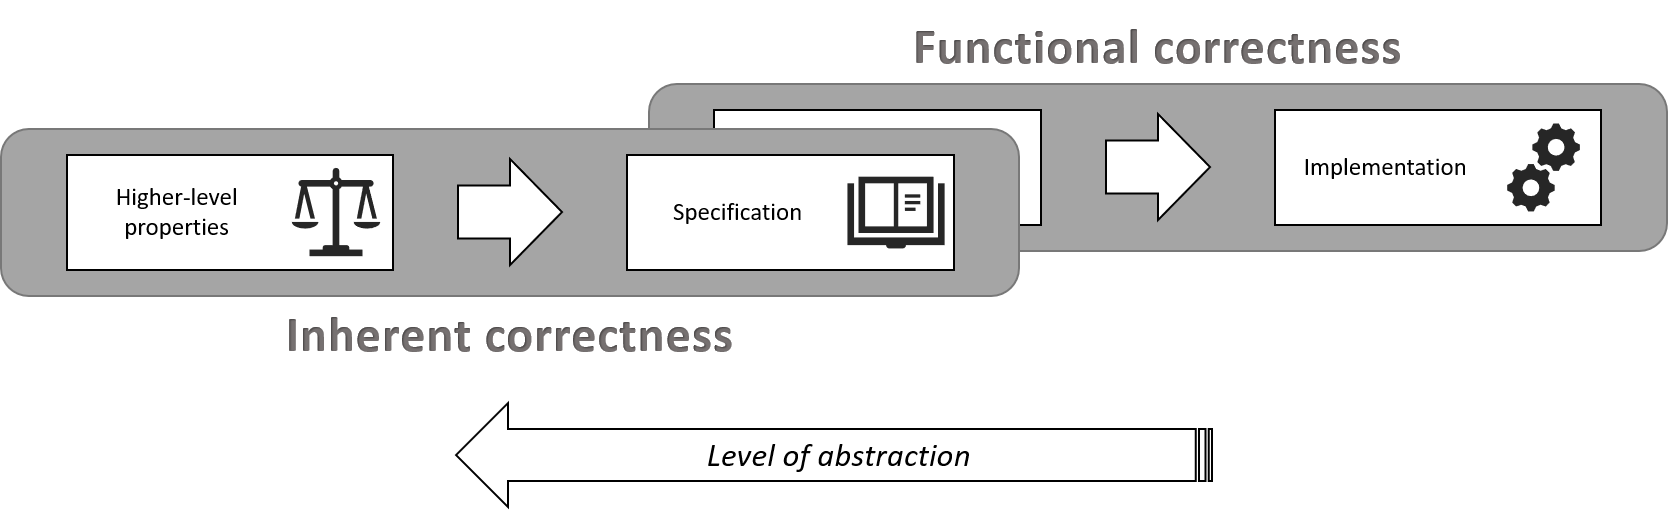
\includegraphics[width=\textwidth]{figures/higher-level-verification.png}
    \caption{Verification of specifications in relation to verification of implementations}
    \label{fig:spec-verification}
\end{figure}

The relation between verifying specifications against higher-level properties and verifying implementations against specifications is depicted in figure \ref{fig:spec-verification}.
This figure illustrates that both of these levels of verification are parallel to each other: Higher-level properties take the same role for specifications as specifications do for implementations.

In the work of \citeauthor{Reid17}, the high-level properties are given by \textcquote[p.88:2]{Reid17}{cross-cutting features} which have the following properties:
\begin{displaycquote}[pp.88:2-3]{Reid17}
    The central design challenge we face is to create a set of properties that:
    \begin{itemize}
        \item express the major guarantees that programmers depend on;
        \item are concise so that architects can easily review and remember the entire set of properties;
        \item are stable so that architectural extensions do not invalidate large numbers of rules;
        \item and that describe the architecture differently from existing specification to reduce the risk of common-mode failure.
    \end{itemize}
\end{displaycquote}.

Cross-cutting features have the downside that they are usually hard to grasp for humans since they require a thorough understanding of the system as a whole, yet are powerful since they often (indirectly) touch many aspects of the specification.

The aspects of the conciseness and stability of the properties implement the idea of a \enquote{constitution} for an \gls{isa} linking back to the paragraphs quoted above.
The first point, however, plays a greater role for the practical applicability of the verification process.
If properties, the architecture is verified against, express \enquote{major guarantees that programmers \textins{can} depend} on, they can be used to aid in usage of the platform, e.g., by \gls{os} engineers to utilize the mechanisms of the architecture correctly and thereby to write secure \glspl{os}.
Lastly, the requirement aimed at reducing the \enquote{risk of common-mode failure} aims at combatting the downsides of other approaches to verify specifications.
\citeauthor{Reid17} lists three commonly used ways of verifying specifications: \textcquote[p.88:2]{Reid17}{by testing specifications against existing implementations; by testing specifications using testsuites used to test implementations; or as a side effect of attempting to formally verify an implementation against a specification}.
These approaches, however, all face the risk of issues with the specification being undetected because the implementation and specification both are affected by the same issue, i.e. the risk of issues being undetected because of common-mode failure.
This risk can be mitigated if the properties the specification will be verified against actually express something \textit{new}.

\citeauthor{Reid17} applies his approach to the ARM M-Class architecture for which not only a natural language but also a machine-readable specification is available.
The machine-readable specification of the ARM M-Class architecture provides the function \asl{TopLevel} which implements the transition of the architecture from one state to another, i.e. a cycle of the processor.
The natural language specification on the other hand mainly consists of rules that constrain the behavior of the architecture in different situations, i.e. constrain the transition relation between architectural states that implicitly is given by the \asl{TopLevel} function.

In principle, these two forms of specification also face the risk of common-mode failures.
In practice, however, it turned out that the natural language specification included several rules that described the behavior of the architecture on a very high-level thus meeting aforementioned requirements.
Using these rules as high-level cross-cutting properties, \citeauthor{Reid17} was able to find 12 bugs in the ARM M-Class specification that despite prior testing had been undiscovered up to this point.

In summary, the aspects of \cite{Reid17} that are relevant for this thesis are:
\begin{enumerate}[label=\alph*)]
    \item the paper argues for why the verification of specifications themselves is important; and
    \item the paper proposes requirements for properties to verify an \gls{isa} against.
\end{enumerate}

Additionally, the paper successfully uses its approach to partially verify the ARM M-Class architecture.
A downside of this work, however, is that it is limited to verifying single processor transactions only.
This approach was chosen due to the nature of the properties from the natural language specification.
These only constrain single transitions of the processor.
To meet these, the formalized properties come in two forms: invariants and properties.
These two types of properties form an inductive proof.
First, it is proven that the initialization procedure of the ARM architecture establishes the invariants, then, it is proven that assuming the invariants no transition of the processor either invalidates an invariant or violates an actual property.
Next to resembling the structure of the natural language specification, this approach promises to be more performant than unbounded model checking.

In this thesis, the work of \cite{Reid17} will be continued: high-level properties will be established to verify \glspl{isa}.
The work in this thesis therefore also is subject to the requirements that have been imposed on the higher-level properties in \cite{Reid17}.
However, the work of \cite{Reid17} will be enhanced by verifying properties applying to multiple processor transitions, i.e. by performing unbounded model checking.
This enhances on three downsides of bounded model checking:
\begin{enumerate}
    \item Counter-examples to properties of \cite{Reid17} are states that also implicitly give a transition into the next state, i.e. an instruction to be executed.
    This makes a counter-example difficult to understand as this state is just some of many during operation of the architecture.
    In contrast, counter-examples in this thesis will be given by an initial state and a series of instructions executed subsequently from this state on, i.e. an actual program.
    It therefore will be easier to understand what exactly happens when a property is violated.
    \item Unbounded model checking gives higher assurance of completeness of the model.
    In \cite{Reid17}, the verification procedure ultimately sets up an inductive proof that allows to make the statement: There is no state that either invalidates an invariant or violates a property.
    In this thesis, the verification procedure will allow for the following statement to be made: There is no program that violates a property.
    This is much broader and there are fewer abstractions to grasp in order to understand what the verification procedure actually does.
    \item Most importantly, the properties in this thesis will be more expressive.
    While in \cite{Reid17}, bounded model checking does limit the scope the properties apply to, the properties themselves are limited - they can only constrain a single transition at a time.
    In this thesis, however, ideas like: \enquote{If first $ X $ and then $ Y $ happens, $ P $ must hold.} which can hardly\footnote{%
        One can think of ways to implement such a property using bounded model checking, e.g., first establish a post-condition for when $ X $ happens and then assume this post- as a pre-condition for $ Y $ happening.
        However, in this a scenario, finding such conditions is non-trivial, it must be further verified that the respective conditions are adequate, e.g., they might be to weak, and establishing these conditions would introduce the need to reverse-engineer how certain actions influence the state.
        This would make them instable and non-concise and, thus, conflict with the self-imposed requirements for the properties.
    } be expressed using bounded model checking.
\end{enumerate}

\section{Information Flow Control}
\label{sec:bg-ifc}

In \citetitle{Ferraiuolo17} \cite{Ferraiuolo17} by \citeauthor{Ferraiuolo17} the authors verify an implementation of the ARM TrustZone architecture by statically type-checking an information flow policy.
To achieve this, they enhance on the already existing \gls{hdl} language SecVerilog, extending its type system to allow more fine grained modelling of information flow policies.
Therefore, the authors verify an implementation against higher-level properties as opposed to verifying a specification as done by \citeauthor{Reid17} in \cite{Reid17}.
This thesis takes this general approach and lifts it to be applied to specifications rather than \glspl{hdl}.

\glspl{hdl} are very much like ordinary programming languages only that they are used to specify electronic circuits.
This use case introduces several novelties to \glspl{hdl} in contrast to programming languages, e.g., type systems are not as rich and usually comprise registers (multiple bits) and wires (one bit). i.e. they resemble much more low level systems.
In context of this thesis, think of an \gls{hdl} as a programming language with a very specific use case.

\citeauthor{Ferraiuolo17} define an \textit{information flow policy} as a lattice of security labels $ (M, \sqcup, \sqcap) $; with $ \sqsubseteq $ being the partial order on $ M $ as induced by the lattice operations supremum $ \sqcup $ and infimum $ \sqcap $.
Intuitively speaking, information labelled with $ a \in M $ is allowed to flow to a sink labelled with $ b \in M $ if and only if $ a \sqsubseteq b $, i.e. information is always allowed to flow up in the lattice but not down.

\begin{example}
    To verify an ARM TrustZone implementation, \citeauthor{Ferraiuolo17} introduce four information flow labels $ \Sigma = \{ \PT, \PU, \CT, \CU \} $ which stand for public/trusted, public/untrusted, confidential/trusted and confidential/untrusted.
    These labels form the information flow policy lattice $ (\Sigma, \sqcup, \sqcap) $ which is depicted in figure \ref{fig:sec-lattice} as a Hasse diagram.
    As we can see, each of these four labels comprises two tokens from two domains of the information flow policy.
    The first of these domains is the one of \textit{confidentiality}, i.e. each label states that a piece of information is either public (\P{}) or confidential (\C{}).
    The second of these domains is the one of \textit{integrity}, i.e. each label states that a piece of information is either trusted (\T{}) or untrusted (\U{}) where \enquote{trusted} marks whether
    the values we deal with are integrous or in other words not malicious.

    \begin{figure}
        \centering
        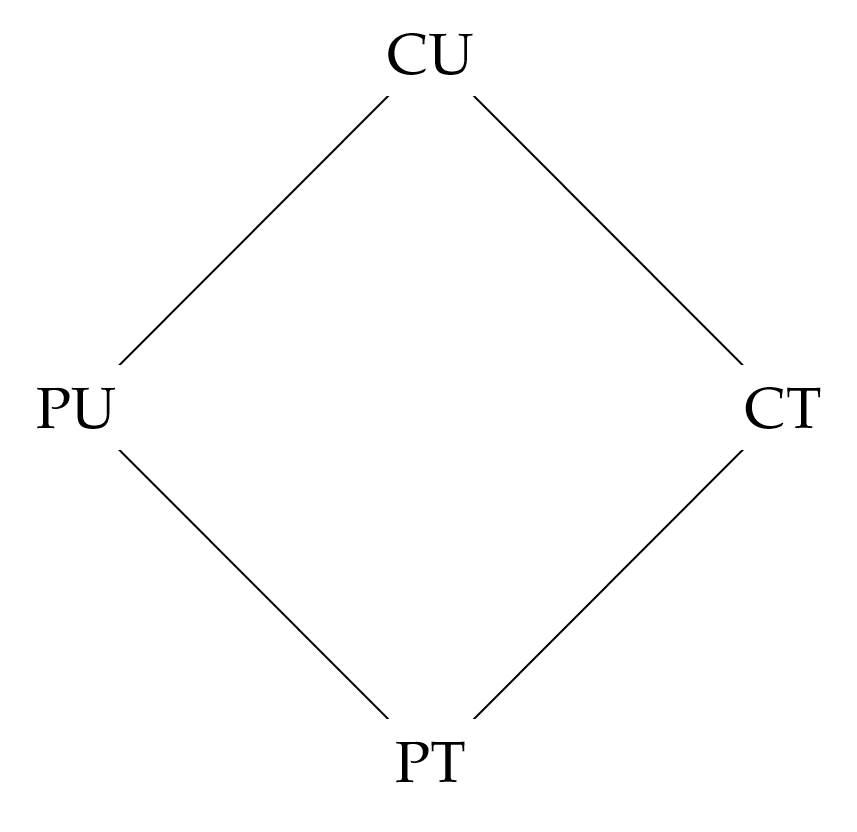
\includegraphics[width=0.4\textwidth]{figures/ifp-lattice.png}
        \caption{Lattice of security labels for verifying an ARM TrustZone implementation displayed as Hasse diagram \cite{Ferraiuolo17}}
        \label{fig:sec-lattice}
    \end{figure}

    It can be seen in the diagram depicting the lattice of security labels (fig. \ref{fig:sec-lattice}) that public information can flow to confidential sinks but not vice versa and that trusted information can flow to untrusted sinks but not vice versa.
    Intuitively, this means that trusted parts of the architecture must only receive trusted data and that confidential data must be handled by confidential parts of the architecture only.
\end{example}

To implement the actual \textit{control} of such an information flow policy, \citeauthor{Ferraiuolo17} introduce the \gls{hdl} language SecVerilogBL that builds upon the \gls{hdl} SecVerilog.
The core of both of these languages when it comes to information flow control is a type-system that adds syntax to the core \gls{hdl} allowing for annotating variables with security labels.
This enables verifying an information flow policy by static type-checking.
In SecVerilog, variables are typed by labels of the respective information flow policy.
The type of a variable is described either by a label $ l \in M $ directly, by the conjunction $ \sqcap $ or disjunction $ \sqcup $ of two labels or by a type-level function $ f $ that maps some program variable $ v $ to a type.
SecVerilogBL enhances on this by tracking security labels not only per variable but also per bit and array element therefore allowing for more fine grained annotation of the \gls{hdl} code but also adding a mechanism to downgrade information.
Since information is not allowed to flow \enquote{down} in the lattice, downgrading can be understood best as a typecast that allows such behavior.
In some \gls{hdl} models, it might be necessary to permit insecure flows of information (in regard to the information flow policy).
In those cases, a programmer can use \lstinline[mathescape]{downgrade(e, $ \tau $)} to annotate the expression \lstinline{e} as being of type $ \tau $, regardless of any prior annotations.
This effectively \textit{grades} the label of a bit of information \textit{down} such that information is not routed to a sink annotated with a label smaller than the information.

In total, SecVerilogBL supports seven ways to express types:
\begin{align*}
    \text{Types } \tau ::= l \mid \tau_1 \sqcup \tau_2 \mid \tau_1 \sqcap \tau_2 \mid x \mapsto \tau \mid f(x) \mid \textit{if $ e^\tau $ $ \tau_t $ $ \tau_f $} \mid \textit{case $ e^\tau $ $ \tau_1 $ \dots $ \tau_n $}
\end{align*}

As can be seen above, types are either given as simple labels of the information flow policy $ (M, \sqcup, \sqcap) $, as the disjunction or conjunction of two types, as a mapping from an index variable $ x $ to some type, as the application of some program variable $ x $ to the function $ f $ or as an $ \textit{if} $- or $ \textit{case} $-expression where $ e^\tau $ is a pure-expression, i.e. side effect free.
Types of the form $ f(x) $ are called \textit{dependent types}.
$ e^\tau $ in $ \textit{if} $- or $ \textit{case} $- expressions might also contain program variables; if it does, these expressions also form dependent types.

Types are of a certain kind:
\begin{align*}
    \text{Kinds } k ::= l \mid \texttt{int} \rightarrow k
\end{align*}

Any type is of kind $ l $.
Furthermore, the type $ x \mapsto \tau $ is of kind $ \texttt{int} \rightarrow k $ where $ k $ is the kind of $ \tau $.
However, when type-checking is performed, types of kind $ l $ are lifted to be of kind $ \texttt{int} \rightarrow l $ such that every type is a partial function from bit indices to information flow labels.
This construct spares programmers from writing type maps for arrays and bit vectors where the type does not change per bit.
This way, a constant type $ \tau $ of kind $ l $ can be applied to a whole bit vector as for type-checking, $ \tau $ is lifted to $ i \mapsto \tau $ which is of kind $ \texttt{int} \rightarrow l $.

\begin{example}
    The following snippet shows the type annotation of parts of a register file definition in SecVerilogBL:
    \begin{lstlisting}[
        language=SecVerilogBL,
        label={snpt:reg-file},
        caption={A register file code segment \cite{Ferraiuolo17}}
    ]
        reg [0:31] {world(ns)} read;
        reg [0:31] { i -> j -> world(reg_ns[i]) } mem[0:1023];
        reg {PT} reg_ns [0:1023];
        (*\dots*)
        if(ns == 1) begin (*\label{ln:assignment}*)
            read = (reg_ns[read_addr] == 1) ?
                mem[read_addr] : 32'b0;
        end else begin
        (*\dots*)
    \end{lstlisting}

    In this example, the variable \lstinline{ns} refers to the \textit{security state} of the ARM TrustZone architecture.
    The ARM TrustZone architecture not only spoorts different privilege but also security states which can either be secure-state (meant to handle confidential data) or non-secure-state (meant to handle only non-confidential data).
    The variable \lstinline{ns} in the implementation of the ARM TrustZone architecture by \citeauthor{Ferraiuolo17} indicates whether the architecture currently is in secure- or non-secure-state.

    The variables \lstinline{read} and \lstinline{reg_ns} illustrate the purpose of lifting types to higher kinds.
    Both types \lstinline{world(ns)} and \lstinline{PT} are of kind $ l $, yet they are used to annotate variables that store more than one bit.
    Because \lstinline{read} is a register with 32 bits, \lstinline{world(ns)} is lifted to \lstinline{i -> world(ns)}, i.e. each element of \lstinline{read} is of the dependent type \lstinline{world(ns)}.
    Similarly, since \lstinline{reg_ns} is an array of 1024 registers of width 1, \lstinline{PT} is lifted to \lstinline{i -> j -> PT}, i.e. each array element is of type \lstinline{j -> PT} and  each array element's bits are of type \lstinline{PT}.

    Starting in line \ref{ln:assignment}, it can be seen how dependent types work in practice.
    The function \lstinline{world} maps 0 to \lstinline{CT} and 1 to \lstinline{PU}.
    The \lstinline{if}-statement first checks whether \lstinline{ns} equals 1, in which case \lstinline{read} would be of type \lstinline{PU}.
    If \lstinline{ns} in fact equals 1, furthermore, the register \lstinline{read} shall be written with \lstinline{mem[read_addr]} but only if the type of that also is of \lstinline{PU} which is checked by ensuring that \lstinline{reg_ns[read_addr]} also equals one.
    Since each element's type of \lstinline{mem} depends on \lstinline{reg_ns}, this assignment is safe since obviously, a variable annotated with type \lstinline{PU} can be written with a value of the same type.

    If this check was omitted and \lstinline{ns == 1}, \lstinline{read} would be written with \lstinline{mem[read_addr]} when \lstinline{reg_ns[read_addr] == 0}, a variable of type \lstinline{PU} would be written with a value of type \lstinline{CT}.
    But since $ \CT \not \sqsubseteq \PU $, this would result in a type-checker error.
\end{example}

The details of this type-system are given by a collection of typing rules.
These rules are written as proofs of sequent calculus.

\begin{example}
    Consider this example of a proof written in sequent calculus:
    \begin{prooftree}
        \AxiomC{$ A $}
        \AxiomC{$ B $}
        \BinaryInfC{$ C $}
    \end{prooftree}

    This proof states that the formula $ C $ can be derived from the formulas $ A $ and $ B $ or more formally that: $ A, B \vdash C $.
\end{example}

In the context of type systems, formulas used in proofs of sequent calculus often are so called \textcquote{Ferraiuolo17}{typing judgements} where some \textit{environment} types some \textit{expression}, e.g., if $ X $ is a type environment, $ x $ an expression and $ \tau $ a type, one possible typing judgement would be $ X \vdash x : \tau $ which means that $ x $ is of type $ \tau $ under the environment $ X $.
In \cite{Ferraiuolo17} three such environments are introduced:

\begin{description}
    \item[Standard environment] $ \Gamma $ maps variables to their respective type $ \tau $.
    \item[Width environment] $ \W $ maps variables to their respective bit vector length.
    \item[Kind environment] $ \Theta $ maps types $ \tau $ to their respective kind $ k $.
\end{description}

\citeauthor{Ferraiuolo17} introduce eight typing rules; these are for constant expressions and variables, logical and arithmetic expressions, bit vector concatenation and shifting as well as array indexing.
An overview of some typing rules of \cite{Ferraiuolo17} are depicted in figure \ref{fig:type-rules}\footnote{%
    It will turn out that only these typing rules are relevant in context of this thesis.
}.
The most simple type system rule probably is T-Const which types constant expressions $ n $.
These are always of type $ \bot $, i.e. \PT, and of the corresponding width $ w $.
The other type system rules share a pattern.
They assume one or two expressions ($ e $ or $ e_1 $ and $ e_2 $) to be typed in $ \Gamma; \W; \Theta $ and ensure that their corresponding types ($ \tau $ or $ \tau_1 $ and $ \tau_2 $) are of the right kind in $ \Theta $.
Then, they create a new type ($ \tau $ or $ \tau' $) and infer a type judgement for a new expression involving $ e $, $ e_1 $ or $ e_2 $ and in some cases a constant $ n $.
This structure of type system rules follows the pattern of an inductive proof or inductive definition of a set where T-Const and T-Var (the typing rule for variables) are the start of induction.

When the SecVerilogBL code is being type-checked, it is verified whether all right sides of assignments are $ \sqsubseteq $-greater than the respective left sides taken together with the label of the program counter.
This means that information is only considered trusted if also the program counter can be considered to be trusted and data is considered to be confidential if either the data itself or the program counter is confidential.

\begin{figure}
    \centering
    \begin{subfigure}[t]{.5\linewidth}
        \begin{prooftree}
            \AxiomC{}
            \UnaryInfC{$ \Gamma; \W; \Theta \vdash n: \bot, w $}
        \end{prooftree}
        \caption{T-Const}
    \end{subfigure}

    \begin{subfigure}[t]{.5\linewidth}
        \begin{prooftree}
            \alwaysNoLine
            \AxiomC{$ \Gamma; \W; \Theta \vdash e_1 : \tau_1, w $}
            \UnaryInfC{$ \Theta \vdash \tau_1 : \texttt{int} \rightarrow l $}

            \AxiomC{$ \Gamma; \W; \Theta \vdash e_2 : \tau_2, w $}
            \UnaryInfC{$ \Theta \vdash \tau_2 : \texttt{int} \rightarrow l $}

            \BinaryInfC{$ \tau = i \mapsto \tau_1( i) \sqcup \tau_2(i) $}

            \singleLine
            \UnaryInfC{$ \Gamma; \W; \Theta \vdash e_1 \circ e_2 : \tau, w $}
        \end{prooftree}
        \caption{T-Logical for $ \circ \in \{ \land, \lor \} $}
    \end{subfigure}

    \begin{subfigure}[t]{.5\linewidth}
        \begin{prooftree}
            \alwaysNoLine
            \AxiomC{$ \Gamma; \W; \Theta \vdash e_1 : \tau_1, w $}
            \UnaryInfC{$ \Theta \vdash \tau_1 : \texttt{int} \rightarrow l $}

            \AxiomC{$ \Gamma; \W; \Theta \vdash e_1 : \tau_2, w $}
            \UnaryInfC{$ \Theta \vdash \tau_2 : \texttt{int} \rightarrow l $}

            \BinaryInfC{$ \tau = i \mapsto \bigsqcup_{j \in [1, i]} (\tau_1(j) \sqcup \tau_2(j)) $}

            \singleLine
            \UnaryInfC{$ \Gamma; \W; \Theta \vdash e_1 \circ e_2 : \tau, w $}
        \end{prooftree}
        \caption{T-Arith for $ \circ \in \{ +, - \} $}
    \end{subfigure}

    \begin{subfigure}[t]{.5\linewidth}
        \begin{prooftree}
            \alwaysNoLine
            \AxiomC{$ \Gamma; \W; \Theta \vdash e : \tau, w $}
            \AxiomC{$ \Theta \vdash \tau : \texttt{int} \rightarrow l $}
            \BinaryInfC{$ \tau' = i \mapsto \ite{(i < n)}{\tau(i - n + 1)}{\bot} $}

            \singleLine
            \UnaryInfC{$ \Gamma; \W; \Theta \vdash e \ll n : \tau', w $}
        \end{prooftree}
        \caption{T-LShift}
    \end{subfigure}

    \begin{subfigure}[t]{.5\linewidth}
        \begin{prooftree}
            \alwaysNoLine
            \AxiomC{$ \Gamma; \W; \Theta \vdash e : \tau, w $}
            \AxiomC{$ \Theta \vdash \tau : \texttt{int} \rightarrow l $}
            \BinaryInfC{$ \tau' = i \mapsto \ite{(i > w - n)}{\bot}{\tau(i + n)} $}

            \singleLine
            \UnaryInfC{$ \Gamma; \W; \Theta \vdash e \gg n : \tau', w $}
        \end{prooftree}
        \caption{T-RShift}
    \end{subfigure}
    \caption{A selection of typing rules for SecVerilogBL expressions \cite{Ferraiuolo17}}
    \label{fig:type-rules}
\end{figure}

In summary, the lattice of security labels taken together with the type system built on top of such a lattice implements three concepts:
\begin{itemize}
    \item A lattice $ (M, \sqcup, \sqcap) $ implements a information flow policy
    \item The typing rules implement information flow tracking
    \item Type-checking implements information flow control
\end{itemize}

\citeauthor{Ferraiuolo17} used these three concepts to verify an implementation of the ARM TrustZone architecture.
In doing so, they first implemented the architecture as a prototype and used the information flow policy to ensure that it did not contain any bugs.
Additionally, they deliberately added bugs to their implementation that have been found in other implementations of the ARM TrustZone architecture and checked whether they were able to find these bugs.
It turned out that their approach was able to detect all bugs besides those which were related to downgrading, i.e. the approach of type-checking information flow control gives a strong security assurances with the exception of bugs due to downgrading expressions.

In this thesis, the concept of an information flow policy, information flow tracking and information flow control will serve to define higher-level properties to verify an \gls{isa} against.
To achieve this, it must be tackled how such an information flow policy as proposed by \citeauthor{Ferraiuolo17} can be applied to \glspl{isa} such that \begin{enumerate*}[label=\alph*)]
    \item the labels can be tracked throughout the architecture by a model checker, and
    \item the policy can be controlled by the model checker.
\end{enumerate*}, i.e. how can the two concepts of information flow tracking and control be implemented using a model checker?

\section{RISC-Architectures}
\label{sec:riscs}

\citetitle{Patterson13} defines the term \gls{isa} as follows:
\begin{displaycquote}[p.22]{Patterson13}
    One of the most important abstractions \textins{in computer design} is the interface between the hardware and the lowest-level software.
    Because of its importance, it is given a special name: the instruction set architecture, or simply architecture, of a computer.
    The instruction set architecture includes anything programmers need to know to make a binary machine language program work correctly, including instructions, I/O devices, and so on.
    Typically, the operating system will encapsulate the details of doing I/O, allocating memory, and other low-level system functions so that application programmers do not need to worry about such details.
\end{displaycquote}

Modern architectures all provide instructions of these categories: instructions for general computation, i.e. bit vector arithmetic, load/store instructions and platform management instructions.

As a target of verification, this thesis will work with \gls{risc} architectures.
In \citetitle{Hennessy12}, \gls{risc} architectures are defined by three main concepts \cite[p.C-4]{Hennessy12}:
\begin{itemize}
    \item RISC architectures are \textit{load/store architectures}, i.e. only load and store instructions affect or touch memory
    \item All other instructions work on registers only and always modify the full width of registers
    \item There are few instructions and their encoding is mostly homogenous
\end{itemize}

The last aspect coined the name \textit{reduced} instruction set computer architecture.
\gls{risc} architectures are often times understood as the counterparts to \gls{cisc} architectures which describe all architectures that do not implement aforementioned \gls{risc}-properties.
The most prominent example of a \gls{cisc} architecture is the x86 architecture which is implemented by most processors manufactured by Intel.

In this section, three \gls{risc} architectures will be introduced: the ARM architecture, MIPS and RISC-V.
It will turn out that these architectures can mainly be differentiated by the balance of customizability vs. feature-richness.
Whereas the RISC-V architecture is most customizable it also supports the fewest features (not including custom extensions).
On the other hand, the ARM architecture is very feature-rich but not very much customizable.
The MIPS architecture strikes a middle-ground of these two extremes.

The goal of this section is to illustrate the features and fundamental design concepts that come with contemporary \gls{risc} architectures.
The decision towards focusing on \gls{risc} architectures as a target of verification was made because their simpler approach to \glspl{isa} makes them far easier to analyze and model than \gls{cisc} processors.
Using a \gls{risc} architecture will allow for implementing an architecture in scope of this thesis while the results will still be applicable and comparable to real-world \glspl{isa} that are in use as of today.
Introducing more than one \gls{risc} architectures will allow us to choose parts to exclude in the verification model without harming our results.

\subsection{Arm}

The ARM architecture defines three architecture \textit{profiles}:
\begin{itemize}
    \item The generic \textit{application profile} ARMv8-A,
    \item the \textit{real-time profile} ARMv8-R designed for deployment scenarios in which real-time responses from a processor is crucial, e.g., in aviation,
    \item and the \textit{microcontroller} profile ARMv8-M aimed at embedded systems.
\end{itemize}

Here, the ARMv8-A profile will be put into focus.
The \citetitle{Armv8} \cite{Armv8} introduces the ARM A-class architecture as a \gls{risc} architecture with three key properties:
\begin{displaycquote}[p.A1-34]{Armv8}
    \begin{itemize}
        \item A large uniform register file.
        \item A load/store architecture, where data-processing operations only operate on register contents, not directly on memory contents.
        \item Simple addressing modes, with all load/store addresses determined from register contents and instruction fields only.
    \end{itemize}
\end{displaycquote}

These properties already meet most of the aspects of \gls{risc} architectures as defined in \cite{Hennessy12}.
When it comes to the aspect of a homogenous instruction set, the ARM architecture makes some trade-offs on this aspect to support the three profiles available.
The ARM architecture supports three instruction sets: A64, a fixed-length 32-bit encoded instruction set for 64-bit systems, A32, a fixed-length 32-bit encoded instruction set for 32-bit systems, and T32, a variable-length instruction set that uses both 16- and 32-bit encodings to support compressed instructions.
The ARMv8-A architecture eases the challenge of correctly decoding these different instruction sets by the concept of \textit{execution states}.
The ARMv8-A supports two of these execution states: AArch64, a 64-bit execution state, and AArch32, a 32-bit execution state.
An ARM A-class processor can receive A64 instructions when in the AArch64 execution state and A32 or T32 instructions when in the AArch32 execution state.

The ARMv8-A specification defines how the processor interacts with memory which includes the specification of a cache and a memory model covering virtual addresses, memory access order control, memory access synchronization, and application level memory restrictions.
Furthermore, it is defined how processors work in a multi-processor setup and how debugging of the architecture works.
The ARMv8-A architecture also supports floating point and vector arithmetic.

If these features do not suffice for a specific use-case, there are nine optional extensions available that can be supported by an ARMv8-A processor including an extension for accelerating cryptographic tasks, for enhancing the reliability, availability and serviceability of the processor, for monitoring and profiling, for enhanced vector arithmetic, and for memory partitioning.

As for registers, the ARMv8-A architecture supports the most versatile types of registers of all \gls{risc} architectures to be compared in this thesis.
Depending on the execution state, 13 to 31 32- or 64-bit registers are supported.
Additionally, there is a \gls{pc}, a dedicated \gls{sp} and some exception link registers.
A general purpose register is used as the standard \gls{lr}.
Furthermore, there are 32 64- or 128-bit registers for floating point and vector arithmetic and a collection of \glspl{csr} that hold status information of the architecture.

\subsection{MIPS}

As opposed to the ARM architecture, the MIPS architecture supports a smaller range of registers and fewer features by default, i.e. without extensions.
It is introduced in \citetitle{MIPS} \cite{MIPS} as: \textcquote[p.21]{MIPS}{based on a fixed-length, regularly encoded instruction set \textelp{which} uses a load/store data model, in which all operations are performed on operands in processor registers, and main memory is accessed only by load and store instructions}.
As for the aspect of a large, uniform register file, MIPS supports 32 32- or 64-bit registers the first of which is hardwired to zero, a \gls{pc} and some \glspl{csr}.
Contrary to the ARM architecture, there are no dedicated \glspl{lr} or \gls{sp}.
As indicated by the options for register width, MIPS supports both a 32- and a 64-bit architecture and instruction sets.

MIPS comes with less features (not including custom extensions) than the ARM architecture; the specification only touches memory interaction including memory virtualization and cache, debugging and the interaction with a standard coprocessor that implements floating point arithmetic.
MIPS, however, is far more customizable than the ARM architecture.
Whereas in case of the latter, customizability is only given by choosing different extensions, a MIPS processor does not need to implement all features defined in the specification to be MIPS compliant.
Certain features can be left out which is called \textit{subsetting} of the architecture.
Additionally to that, MIPS allows to extend the architecture by user defined instructions, compressed instructions, enhanced media processing, enhanced geometry processing, smart card or object interaction, signal processing, multi threading, \gls{os} virtualization, vector arithmetic and an extensions aimed specifically at microcontrollers.

\subsection{RISC-V}
\label{sec:bg-riscv}

RISC-V was originally presented in the technical report \citetitle{RiscVISA-org} in May 2011 \cite{RiscVISA-org} and has undergone many changes since then.
RISC-V's architectural specification is divided into two volumes: volume 1 specifies the base user-level \gls{isa} which is separated into several modules whereas volume 2 defines the privileged architecture and instruction set but is still only available as a draft.
The privileged architecture is not divided into modules but rather \textit{functional groups} that define certain aspects of privileged computing.
Such groups include for example machine- and supervisor-level \glspl{isa} or the description of a platform level interrupt controller.

This thesis works with version 2.2 of volume 1 \cite{RiscVISA} and version 1.1 of volume 2 \cite{RiscVISAP}.
RISC-V understands itself as a highly customizable architecture.
Currently, there are four variants of a base integer instruction set - one of which must be implemented by any RISC-V processor - and 13 optional extensions.
The base integer instruction sets include instructions for integer arithmetic, memory operations (loads and stores), control transfer (jumps and branches) and platform management (environment calls and status register operations).
The base integer instruction sets mainly differ in the word-size and register number.
To cope with these differences, they also make small adjustments to some functionalities but only slightly change the instruction set itself.
These four base integer instruction sets are given by:
\begin{description}
    \item[RV32I] Base integer instruction  for a 32-bit architecture
    \item[RV32E] Base integer instruction set for embedded computing
    \item[RV64I] Base integer instruction set for a 64-bit architecture
    \item[RV128I] Base integer instruction set for a 128-bit architecture
\end{description}

The RISC-V manual differentiates between standard and non-standard extensions but only introduces standard ones.
A standard extension is meant to be compatible with any other standard extension and should be \textcquote{RiscVISA}{generally useful} whilst non-standard extensions might add support for more niche use-cases and do not need to be compatible with all standard extensions.

The set of functionalities offered by standard extensions begins at a low level with the probably most mundane being the standard extension for integer multiplication and division.
You can find a list of all standard extensions in table \ref{tbl:rv-exts}.

\begin{table}
    \centering
    \begin{tabular}{| c | l |}
        \hline
        \textbf{M} & Integer multiplication and division \\
        \textbf{A} & Atomic instructions \\
        \textbf{F} & Single-precision floating-point arithmetic \\
        \textbf{D} & Double-precision floating-point arithmetic \\
        \textbf{Q} & Quad-precision floating-point arithmetic \\
        \textbf{L} & Decimal floating-point arithmetic \\
        \textbf{C} & Compressed instructions \\
        \textbf{B} & Bit manipulation \\
        \textbf{J} & Dynamically translated languages \\
        \textbf{T} & Transactional memory \\
        \textbf{P} & Packed-SIMD instructions \\
        \textbf{V} & Vector operations \\
        \textbf{N} & User-level interrupts \\
        \hline
    \end{tabular}
    \caption{All RISC-V standard extensions}
    \label{tbl:rv-exts}
\end{table}

A subset of the RISC-V \gls{isa} is described by a so called \textcquote{RiscVISA}{\gls{isa} naming string} which comes in the following form:

\begin{grammar}
    <naming-string> ::= `RV' (`32' | `64' | `128') (`I' | `E') <extensions>
\end{grammar}

An example for a naming string is the very common \gls{isa}-subset RV64IMAFD which officially is abbreviated by RV64G.
This subset includes the integer multiplication and division, user-level interrupts, atomic instructions, single-precision and double-precision floating-point arithmetic extensions.

A RISC-V core consists of multiple \glspl{hart}.
Each \gls{hart} controls its own set of registers including a \gls{pc} and is equipped with its own instruction fetch unit.
However, multiple \glspl{hart} share the same memory.

A \gls{hart} might either control 16 or 32 general purpose registers which are named from x0 to x31.
All but one instruction sets support 32 general purpose registers whereas the exception to this is the base instruction set aimed at embedded computing, RV32E, which only supports 16 general purpose registers.

Similarly to the MIPS architecture, the first of these general purpose registers is hardwired to zero and for example can be used as a target register when the result of an instruction is not needed.
Also, there is no dedicated \gls{lr} or \gls{sp}.
RISC-V supports up to 4096 \glspl{csr}.

\subsection{Summary}

In the previous sections, it was shown how the ARM, MIPS, and RISC-V architectures implement the three main properties of \cite{Hennessy12} characterizing \gls{risc} architectures: a small and uniformly encoded instruction set, a large and uniform register file and a load/store architecture.
Whereas the ARM architecture supported customizability only by a list of extensions and MIPS added user defined instructions and allowed subsetting its core specification, RISC-V took the idea of customizability and made it part of the core idea of the architecture.
RISC-V supports the most simple yet fully specified processor in form of the RV32E.
It was this degree of customizability and simplicity that led to the decision to use RISC-V as a target of verification in this thesis.
There are no major features RISC-V lacks in that are crucial to the concept of a \gls{risc} architecture.

\section{The Ecosystem of an ISA}
\label{sec:ecosystem}

\glspl{isa} are embedded in a larger context.
The goal of this thesis is to verify an \gls{isa} against higher-level properties.
For this undertaking to be worthwhile, it must be clear where the limitations of these properties lie.

An \gls{isa} is an interface offered by hardware which is used by binary programs and in particular \glspl{os}.
It serves an analogous purpose to a programming language.
The latter is used by programs and \glspl{os} as a specification of the input language to compilers, the former is used by compilers and \glspl{os} as a specification of the input language to the actual hardware.
Yet, this thesis does not verify \glspl{os}, programs, compilers or hardware.
With these boundaries in mind, it must be decided what will be incorporated in the model that will be developed over the course of this thesis.

\subsection{Microarchitectures}
\label{sec:microarchs}

The hardware implementation of an \gls{isa} is called \textit{microarchitecture}.
Such implementations usually incorporate sophisticated features that speed up operation of the chip such as pipelining.
Instructions that are defined as part of an \gls{isa} are not atomic in regard to their execution; there usually are five steps that must be taken in order to execute an instruction, the so called Von-Neumann cycle (cf. \cite[p.286]{Patterson13}):
\begin{enumerate}
    \item Instruction fetch - load the instruction from memory
    \item Instruction decode and register file read - Read the fetched instruction and read registers targeted by the instruction
    \item Execution or address calculation - Use the \gls{alu} to perform the instruction or to calculate a memory address
    \item Data memory access - Access the memory for a read or write
    \item Write back - Store the result of the instruction in a register
\end{enumerate}
The microarchitecture comprises functional modules that implement each of this steps.
To use the microarchitecture to the fullest, it is much more efficient to use these modules in a pipeline where for example after the first instruction has been fetched and handed to the module decoding it, the next instruction is fetched in parallel.
In an ideal scenario, executing $ n $ instructions using a pipeline of length $ p $ only takes $ n + p - 1 $ cycles whereas without pipelining this would take $ n * p $ cycles.

Such features introduce \textit{sub-architectural state}.
For example, pipelining introduces the \textit{state} of the pipeline which is sub-architecturally because it is independent of the \gls{isa}.
An accurate model of an \gls{isa} that aims to be true to current implementations would need to include such features.
However, since the goal of this thesis is to verify an \gls{isa}, the model to be verified must be implementation independent.
Furthermore, verifying such hardware features falls in the realm of functional correctness.
Features such as pipelining face the risk that an implementation turns out to violate the \gls{isa} because instructions might execute not as they should.
Adding to the first argument of the model not being implementation independent, including sub-architectural state into the model would lead to an indirect verification of the functional correctness of such parts, i.e. whether they truly implement the \gls{isa}.
This thesis, however, is not about verifying how pipelining can be implemented correctly but about \textit{higher-level} properties of \glspl{isa}.

Additionally, aspects of the functional correctness of an implementation towards the \gls{isa} are served adequately by existing methods:
In \cite{Mukherjee16} attempts to verify hardware in general have been proposed and implementations of processors have been verified against higher-level properties in \cite{Zhang15, Beatty94, Berezin98, Trippel19} or against their actual specifications in form of an \glspl{isa} in \cite{Reid16, RISCV-formal}.
In particular, pipelining has been verified in \cite{Burch94}.

\subsection{Virtual Memory}
\label{sec:virtual-memory}

Virtual memory is usually managed by \glspl{os} and mostly serves two purposes: \textcquote[p.428]{Patterson13}{to allow efficient and safe sharing of memory along multiple programs \textelp{} and to remove the programming burdens of small, limited amount of main memory.}
Virtual memory is a system that replaces physical memory addresses with virtual ones.
The virtual address space usually is bigger than the physical.
Memory is divided into pages with a virtual address being made up of a page index and a page offset.
On accessing an address, the page index is translated to a physical memory address which taken together with the page offset results in the respective physical memory address.
This allows programs to treat their \enquote{personal} address space as continuous whereas in reality it comprises several pages of memory scattered all over physical memory.

Virtual memory usually is part of \glspl{isa}; e.g., the ARM architecture includes the specification of the \gls{mmu} which translates addresses and is programmed by an \gls{os} via system registers (cf. chapter D5 \cite{Armv8}).
The RISC-V specification also includes a system for managing virtual memory with an address space of 32, 39, or 48 bits (cf. section 4 \cite{RiscVISAP}).
Here, the setup of virtual memory also is delegated to an \gls{os} and can be configured by programming system registers.

Again, it is important that hardware modules that handle address translation work functionally correct.
This has been covered in \cite{Dalinger05} and will be left out in this context to keep the target of verification implementation independent.
It can be verified whether virtual memory management systems \textit{correctly} isolate programs and correctly setup virtual memory.
This problem, however, falls in the realm of \gls{os} verification and has been touched by \cite{Vaynberg12} in detail.
The reader is also referenced to the seL4 project \cite{Klein09} in which a complete kernel was formally verified.

With this research in mind, it was decided not to include virtual memory addresses in the model to be targeted for verification.
Mechanisms that provide isolation between memory regions will be modelled, however, the model does not benefit from a simulation of virtual memory addresses.
Addresses will be treated as physical ones throughout this thesis.

\subsection{Threat Model}
\label{sec:threat-model}

Now that two concepts that touch most architectures have been ruled out, namely sub-architectural hardware mechanisms or virtual memory, this section will give a positive description of what \textit{will} be part of the model.
This leads to the question of the threat model of the higher-level properties to be verified.

A key feature of modern architectures that is used by modern \glspl{os} is to have different privileges levels.
For example, the RISC-V architecture supports up to three different privilege levels; from lowest to highest: user-mode, supervisor-mode and machine-mode.
Higher privilege levels usually give access to more system control registers, specific instructions and often times work hand in hand with specific semantics of system registers, e.g., RISC-V supports physical memory regions which support settings for each privilege level, i.e. certain regions of physical memory can be set readable to machine- but not user-mode, etc.

In a sense, privilege modes play a similar role to virtual memory.
Both concepts are used by \glspl{os} in very fundamental ways and therefore are relevant for the security of a system as a whole.
Yet, hardware only supports the foundation for virtual memory, i.e. address translation and the possibility to set properties of memory regions, whereas privilege levels and interrupts are systems offered to the \gls{os} and implemented in the hardware completely.
\glspl{os} use memory management systems to offer virtual memory to applications but rely on privilege levels to function at all.
While it was argued that verification of virtual memory systems should be targeted at \glspl{os} the same cannot be said for the verification of privilege levels.
Thus, this thesis will focus on the mechanics of privilege levels in the process of verification.

This links back to \cite{Reid17}; recall that one goal of this work was to \textcquote[p.88:2]{Reid17}{express the major guarantees that programmers depend on}.
Since \glspl{os} heavily rely on correct implementations of privilege levels and especially the mechanics to transition between those, it is of specific interest to verify high-level properties about the workings of these mechanisms which will lead to insights in these guarantees.

Privilege levels go hand in hand with interrupt and exception handling.
Interrupts generally are used in \glspl{isa} to transfer control to specific privilege modes or programs, e.g., whenever one presses a key on a keyboard, a keyboard interrupt is generated that is handled by the appropriate device driver and propagated by the \gls{os} to the correct application, e.g., your text editor or shell.
Exceptions usually refer to error conditions that arise during computation.
For example, coming back to physical memory regions in RISC-V, if user-mode would attempt to read from a region unreadable to it an exception would be generated.
It is the obligation of software running in machine-mode to handle such error conditions - usually related software comes as part of an \gls{os}.

To put the mechanics of transitions between privilege levels to a test, the threat model taken as a basis of the verification process in this thesis is the following\footnote{%
    Since the decision to work with RISC-V in this thesis has already been made, the threat model was phrased with this in mind.
}:
\begin{quote}
    \itshape
    Assume that user-mode has been completely compromised.
    Is there any way it can gain access to secret data handled by machine-mode or it can gain control over machine-mode?
\end{quote}

Intuitively, linking privilege modes back to \glspl{os}: Assume you have a malicious app on your computer.
Is there any way it can use the \gls{isa} that is built into your computer to either access secret data or hijack your \gls{os}?

This goes beyond what can be verified purely in terms of hardware verification as discussed in section \ref{sec:microarchs}.
Even if it could be assumed that the hardware your computer is running on accurately implements the respective \gls{isa} - as long as the design of that \gls{isa} is flawed in the sense that it has security holes baked into it, i.e. into the \gls{api} that is used by the \gls{os} to give instructions to the hardware, any attempt to build a secure system is pointless\footnote{%
    Research verifying hardware against higher-level properties has been discussed in section \ref{sec:microarchs}.
    Without going into details on this research, the approach of this thesis still is an important addition to this research as it is more general, i.e. implementation independent whereas hardware verification by its very nature is implementation dependent.
}.

In this threat model, timing channels are not considered.
With recent microarchitectural-attacks (cf. Meltdown \cite{Lipp2018meltdown} and Spectre \cite{Kocher2018spectre}) these become more and more relevant, however, when considering \glspl{isa} they are of secondary importance.

\section{Model Checking}
\label{sec:model-checking}

Model checking is a technique that falls into the domain of formal verification.
It is one way to prove that a given system complies with a given specification.
\citeauthor{Baier08} introduce model checking in their book \citetitle{Baier08} \cite{Baier08} as:
\begin{displaycquote}[p.7ff.]{Baier08}
    \textit{Model-based} verification techniques are based on models describing the possible system behavior in a mathematically precise and unambiguous manner. \textelp{}
    This provides the basis for a whole range of verification techniques ranging from an exhaustive exploration (model checking) to experiments with a restrictive set of scenarios in the model (simulation), or in reality (testing). \textelp{}

    Model checking is a verification technique that explores all possible system states in a brute-force manner.
    Similar to a computer chess program that checks possible moves, a model checker, the software tool that performs the model checking, examines all possible system scenarios in a systematic manner.
    In this way, it can be shown that a given system model truly satisfies a certain property. \textelp{}

    Typical properties that can be checked using model checking are of a qualitative nature:
    Is the generated result OK?,
    Can the system reach a deadlock situation, e.g., when two concurrent programs are waiting for each other and thus halting the entire system?
    But also timing properties can be checked:
    Can a deadlock occur within 1 hour after a system reset?, or, Is a response always received within 8 minutes?
\end{displaycquote}

Model checking therefore deals with two parts: Firstly, a model of some system, secondly, properties formalized on the basis of some specification.
Systems to be model checked come in many forms.
They range from software libraries over hardware designs to embedded controllers.
The same is true for specifications.
Those can be fully fledged \textit{actual} specifications that describe the requirements to a system exhaustively or higher-level properties that generally should apply to systems such as deadlock freeness as mentioned in \cite{Baier08}.

More technically, in model checking some system is taken and transformed into a model using a formal language like PROMELA (cf. section \ref{sec:spin}) and a specification is taken and transformed into a property usually expressed in some formal logic, e.g., \gls{ltl}.
Then it is verified via a model checker whether the system model models the formal property.
Note that \enquote{model} in this context is ambiguous.
On the one hand this term refers to the model of the system as a simplified description; on the other hand, this term refers to the logical models-relation $ \models $ which is actually being checked.

An overview of model checking is given in figure \ref{fig:model-checking}.
There, the idea and purpose of model checking is depicted.
In summary, model checking is a technique that allows to solve the problem of ensuring that a system complies with a specification.
By translating the system into a model and the specification into a formal property this problem can be translated into \textit{checking} whether the model \textit{models} the formal property.

\begin{figure}
    \centering
    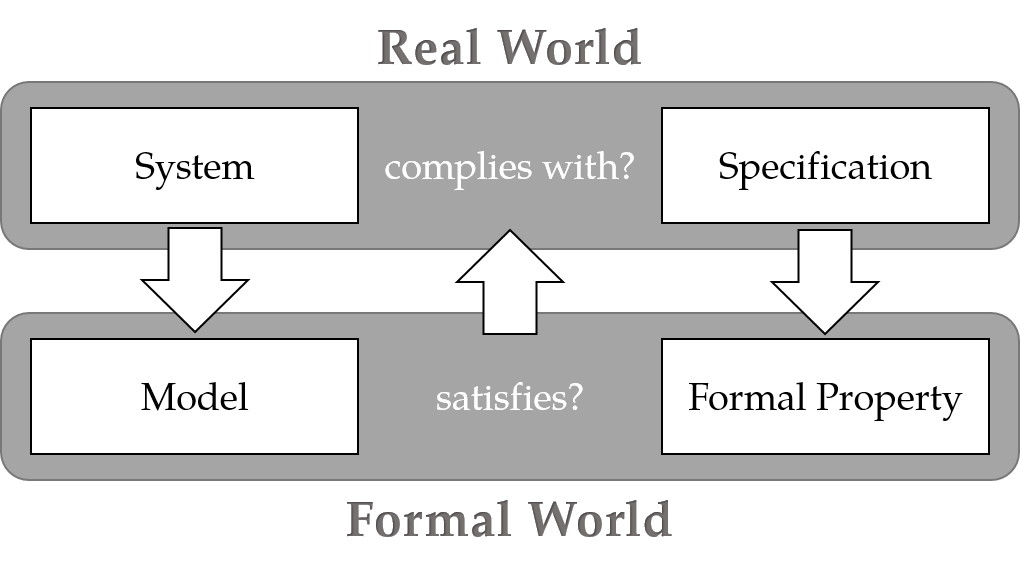
\includegraphics[width=0.7\textwidth]{figures/model-checking.png}
    \caption{Overview of Model Checking}
    \label{fig:model-checking}
\end{figure}

It has already been mentioned in the introduction of both the thesis and this section that the model checker to be used in this thesis is nuXmv.
The aim of this subsection is to introduce nuXmv and two other tools that were taken into consideration for this thesis.
These other two model checkers are called SPIN and SPACER.
By introducing three model checkers, we want to give a feel for all the different flavors of model checkers and be able to argue for why nuXmv was chosen over others.
However, this section does not intend to perform an thorough analysis of contemporary model checkers.

\subsection{SPIN}
\label{sec:spin}

SPIN (which stands for \textit{S}imple \textit{P}romela \textit{IN}terpreter) is a model checker that has been originally developed by Bell Labs and made freely available in the nineties.
As its name suggests, it uses PROMELA as input language.
\citetitle{SpinManual} \cite{SpinManual} which has been used as source for this section, describes SPIN initially as follows:
\begin{displaycquote}[p.1]{SpinManual}
    SPIN can be used to verify correctness requirements for systems of concurrently executing processes.
    The tool works by thoroughly checking either hand-built or mechanically generated models that capture the essential elements of a distributed system's design.
    If a requirement is not satisfied, SPIN can produce a sample execution of the model to demonstrate this.
\end{displaycquote}

As indicated by the quote, SPIN focusses heavily on the verification of distributed or parallel systems.
This is reflected not only in its input language but also in the way how properties are expressed.
For an introduction by example to PROMELA, cf. snippet \ref{snpt:spin-exm}.
PROMELA relies on describing systems as sets of processes that run in parallel where parallel means that each process can advance its state (generally) independent of other processes\footnote{%
    We added the restriction \textit{generally} to the claim because processes can be set up such that they deliberately wait for other processes to send them a message or set some shared state accordingly.
    However, such mechanisms where processes depend on each other always need to be implemented accordingly.
}.

In snippet \ref{snpt:spin-exm}, two processes of the same type \lstinline{user} are declared in line \ref{ln:proc}.
The idea of this snippet is to implement and verify an algorithm that grants these two processes mutually exclusive access to the critical region spanning lines \ref{ln:crit-start}-\ref{ln:crit-end}.
This is ensured by the assertion in line \ref{ln:assert} since variables in SPIN are always initialized to 0 - if two processes had access to the critical region at the same time, \lstinline{cnt} would become 2 at some point.

The details of the protocol implemented in lines \ref{ln:excl-start}-\ref{ln:excl-end} are not relevant for this thesis.
Their purpose is to grant mutual exclusive access to the critical region.
However, this part of code gives an indication for how models written in PROMELA look like.
Besides \lstinline{if} statements and labels similar to those in C (cf. line \ref{ln:label}), PROMELA supports \lstinline{do}-loops to control process execution flow.
\lstinline{do}-loops run indefinitely until they are exited manually by a \lstinline{break} statement.

As data types, PROMELA supports three categories: processes, message channels and data objects.
Data objects comprise atomic data types such as \lstinline{byte}, \lstinline{bool}, \lstinline{int}, etc. as well as complex data type defined by \lstinline{typedef} that define a complex structures that have fields of data objects.
Both atomic data types and complex data types are close to the data types of C.

\begin{figure}
    \begin{lstlisting}[
        caption={Faulty Mutual Exclusion Algorithm Implemented in PROMELA \cite{SpinManual}},
        label={snpt:spin-exm}
    ]
        byte cnt;
        byte x, y, z;

        active [2] proctype user() (*\label{ln:proc}*)
        {
            byte me = _pid + 1;
        again: (*\label{ln:label}*)
            x = me; (*\label{ln:excl-start}*)
            if
            :: (y == 0 || y == me) -> skip
            :: else -> goto again
            fi;

            z = me;
            if
            :: (x == me) -> skip
            :: else -> goto again
            fi;

            y = me;
            if (z = me) -> skip
            :: else -> goto again
            fi; (*\label{ln:excl-end}*)

            cnt++; (*\label{ln:crit-start}*)
            assert(cnt == 1); (*\label{ln:assert}*)
            cnt--; (*\label{ln:crit-end}*)
            goto again
        }
    \end{lstlisting}
\end{figure}

Snippet \ref{snpt:spin-output} shows the output when verifying snippet \ref{snpt:spin-exm} with SPIN where it is assumed that latter snippet was written into a file called \lstinline{mutex_flaw.pml}.
The lines of the output are structured as follows: at the beginning of each line, a step index indicating the progress of all processes can be seen, whilst \lstinline{proc X (NAME)} indicates the process that has made progress by its ID and name.
The rest of the line \lstinline{line X ... [CODE]} shows the code executed by the process along with the corresponding line number in the source file\footnote{%
    In this case, line numbers do not fully align with snippet \ref{snpt:spin-exm}.
}.
Notice, how processes 0 and 1 progress completely independently from each other, executing code on a line by line basis where each step of any process counts as a state transition of the whole model.

\begin{figure}
    \begin{lstlisting}[
        caption={SPIN Example Output \cite{SpinManual}},
        label={snpt:spin-output}
    ]
        1:  proc    1 (user) line   5 ... [x = me]
        2:  proc    1 (user) line   8 ... [(((y==0) || (y==me)))]
        3:  proc    1 (user) line  10 ... [z = me]
        4:  proc    1 (user) line  13 ... [((x = me))]
        5:  proc    0 (user) line   5 ... [x = me]
        6:  proc    0 (user) line   8 ... [(((y==0) || (y==me)))]
        7:  proc    1 (user) line  15 ... [y = me]
        8:  proc    1 (user) line  18 ... [((z = me))]
        9:  proc    1 (user) line  22 ... [cnt = cnt+1]
        10: proc    0 (user) line  10 ... [z = me]
        11: proc    0 (user) line  13 ... [((x = me))]
        12: proc    0 (user) line  15 ... [y = me]
        13: proc    0 (user) line  18 ... [((z==me))]
        14: proc    0 (user) line  22 ... [cnt = (cnt+1)]
        spin: line 223 of "mutex_flaw.pml", Error: assertion violated
        spin: text of failed assertion: assert((cnt==1))
        15: proc    0 (user) line  23 ... [assert((cnt==1))]
        spin: trail ends after 15 steps
        # processes: 2
            cnt = 2
            x = 1
            y = 1
            z = 1
        15: proc    1 (user) line  23 "mutex_flaw.pml" (state 20)
        15: proc    0 (user) line  24 "mutex_flaw.pml" (state 21)
        2 processes created
    \end{lstlisting}
\end{figure}

Assertions, however, are not the only way to express properties of PROMELA models for SPIN.
Furthermore, there are:
\begin{itemize}
    \item Labels
    \item Never claims
    \item Trace assertions
\end{itemize}

Labels have already been introduced informally along with snippet \ref{snpt:spin-exm}.
To express properties about a model, certain types of labels can be used to give semantics to process state.
For example, you can label a certain part of process code as end-state that might look like an idling-state to SPIN by default.
Idling- and end-states are important to SPIN when it's checking for deadlock-freeness of systems.
By default, if all processes are in an idling-state and wait for some kind of signal, this state is considered to be a deadlock.
However, in some situations it might be perfectly fine for some of the processes to idle in a specific state which should not contribute towards deadlocks.
Labeling parts of code as end-state contributes towards this.

Never claims are processes themselves.
They run like any other process but must not terminate otherwise they're regarded as failure.
This is the most complex way to express properties and in fact falls together with writing \gls{ltl} properties about a model which will be introduced in section \ref{sec:nuxmv}.
Therefore SPIN allows to express such never properties in \gls{ltl} directly via their command line interface.

The last type of properties, trace assertions, solely deal with message passing and therefore are not relevant to this thesis.

It might be obvious at this point why we decided against using SPIN as the model checker of this thesis.
Its focus on verifying distributed and parallel systems would make implementing an \gls{isa} in it very hard.
In the \textit{Primer and Reference Manual} for SPIN it is written:
\begin{displaycquote}[p.33]{SpinManual}
    \textins{W}e saw that the emphasis in PROMELA models is placed on the coordination and synchronization aspects of a distributed system, and not on its computational aspects. \textelp{}
    The specification language we use for systems verification is therefore deliberately designed to encourage the user to abstract from the purely computational aspects of a design, and to focus on the specification of process interaction at the system level.
\end{displaycquote}

However, the \gls{isa} we will attempt to verify
\begin{enumerate*}[label=\alph*)]
    \item will most likely not include components \enquote{interacting at the system level} and
    \item will be verified on a component level, i.e. computationally as well - even in the case where multiple system level components would be given.
\end{enumerate*}

Furthermore, it is unreasonable to assume that an implementation of instructions of an \gls{isa} could be implemented in a single statement of PROMELA.
Yet, this should be the goal as otherwise as shown in snippet \ref{snpt:spin-output} what is regarded as state by SPIN would not fall together with what is regarded as state in an \gls{isa}.
For an \gls{isa}, one typically would consider the \textit{state} of registers and memory to be the state of the \gls{isa} whilst some instruction advances this state.
However, for SPIN more complex state transitions would result in us not being able to differentiate architectural states of the \gls{isa} natively since the process implementing the \gls{isa} would change state on each line of code executed.
This could be circumvented by using the \lstinline{atomic} keyword offered by PROMELA which lets you wrap a group of PROMELA statements such that they're considered as one atomic statement that advances the process state only by one step.
This, though, would lead to a model consisting of one process all of its code being wrapped by one \lstinline{atomic} statement.
This would massively contradict the key idea of SPIN of simple models being \textit{abstracted} from computationally complex code.
In this case, we would have skipped the whole step of abstracting from some computational model that has distributed components running in parallel.
Not only could this lead to performance issues, it also can be safely assumed that the work for this thesis would be cumbersome and might stumble over obstacles induced by abusing SPIN.

\subsection{\muZ{} \& SPACER}
\label{sec:spacer}

\muZ{} is a Datalog-engine that provides querying fixed points with constraints and has been proposed in \cite{Hoder11}.
According to \textit{An Introduction to Database Systems} \cite[p.790ff]{Date00}, Datalog is a descriptive and querying language that originated in the field of database management systems.
At its core, Datalog programs are sets of \textit{rules} that combine predicates only using variables and constants to Horn-clauses, i.e. disjunctions with one positive literal at maximum.
For example, consider the following rule $ \pi_0 $ which expresses the transitivity of a predicate $ P $:
\begin{equation*}
    \pi_0 := P(a, b) \land P(b, c) \Rightarrow P(a, c)
\end{equation*}
Such programs are then used to \textit{deduct} facts from the set of rules.
To illustrate what this means, we introduce two other rules.
\begin{align*}
    \pi_1 := & P(0, 1) \Rightarrow \top \\
    \pi_2 := & P(a, b) \Rightarrow P(a + 1, b + 1)
\end{align*}
The Datalog-program $ \Pi := \{ \pi_0, \pi_1, \pi_2 \} $ now induces the relation $ < $ in form of the predicate $ P $ on all natural numbers including $ 0 $.
$ \pi_1 $ sets up a start of induction which, stating that $ 0 $ is smaller than $ 1 $.
This is generalized for all natural numbers by $ \pi_2 $.

Whether or not this exact Datalog-program is supported by a given Datalog-engine depends on the extensions implemented by the respective engine.
Our example relies on an extension for scalar operators since we use the $ + $ operator.

As briefly mentioned, Datalog also supports queries.
Datalog queries comprise only one predicate and a special head $ ? $.
\begin{equation*}
    q_0 := P(0, x) \Rightarrow \; ?
\end{equation*}
The result to a query is the set of all values for each variable that make the predicate true.
In this case, the result set would be $ \{ 1, 2, 3, \dots \} $.
If no variables but only constants are given in the query, Datalog simply determines whether the given predicate can be derived for the given constants.

\muZ{} now is a Datalog-engine that comes as part of the SMT solver z3 \cite{Moura08} and adds support for expressing Horn-clauses to it.
For example, consider the implementation of the program $ \Pi $ for \muZ{} as depicted in snippet \ref{snpt:muz-exm}.
This example yields \smt{sat} as result when executed, meaning, that \smt{goal} can be derived from the rules at hand.

\begin{figure}
    \begin{lstlisting}[
        language=SMT2,
        caption={Implementation of $ \Pi $ for \muZ{}},
        label={snpt:muz-exm}
    ]
        (declare-var a Int)
        (declare-var b Int)
        (declare-var c Int)

        (declare-rel ge (Int Int))
        (declare-rel goal ())

        (rule (ge 0 1))                     ; pi_1
        (rule (=>   (ge a b)                ; pi_2
                    (ge (+ a 1) (+ b 1))))
        (rule (=>   (and (ge a b) (ge b c)) ; pi_0
                    (ge a c)))

        (rule (=>   (ge 10 15)
                    goal))
        (query goal)
    \end{lstlisting}
\end{figure}

SPACER \cite{Komuravelli13} is an algorithm that combines two widely implemented approaches of currently available formal verification tools: \gls{2bmc} and \gls{cegar}.
In its implementation, SPACER uses \muZ{} as a backend.
The paper introducing SPACER, \citetitle{Komuravelli13} \cite{Komuravelli13}, describes those techniques as follows:
\begin{displaycquote}[p.1f]{Komuravelli13}
    The key idea of \gls{2bmc} is to iteratively construct an under-approximation \textins{(or refinement)} $ U $ of the target program $ P $ by unwinding its transition relation and check whether $ U $ is safe using \gls{bmc}.
    If $ U $ is unsafe, so is $ P $.
    Otherwise, a proof $ \pi_U $ is produced explaining \textit{why} $ U $ is safe.
    Finally, $ \pi_U $ is generalized (if possible) to a safety proof of $ P $.
    \textelp{}

    Thea idea of \textins{\gls{cegar}} is to iteratively construct, verify, and refine an abstraction (\textit{i.e.}, an over-approximation) of $ P $ based on abstract counterexamples.
\end{displaycquote}

The key to understanding how SPACER works is to understand what under- or over-approximation of programs are.
For the sake of brevity, these concepts will be introduced by example.
Consider the program $ P $ as depicted in snippet \ref{snpt:spacer-p}.
$ P $ performs an integer division with remainder for a natural number \lstinline{n} by a divisor \lstinline{div} storing the results in \lstinline{ratio} and \lstinline{mod}.
Intuitively speaking, $ \hat{P} $ is an under-approximation (or abstraction) of $ P $ if for every part of $ P $ there is a corresponding part of $ \hat{P} $ whose effects are logically entailed by the original part.
Vice versa, $ P $ is an over-approximation of $ \hat{P} $.
An example for an over-approximation of $ P $ in snippet \ref{snpt:over-p} and an example for an under-approximation in snippet \ref{snpt:under-p}.
For abstracting $ P $ to $ \hat{P} $ a couple of lines were removed whilst all other were left untouched\footnote{%
    Note, that formally, under- and over-approximations are defined via control flow graphs.
    The intuition here is that a control flow graph $ G $ over-approximates another control-flow graph $ G' $ if $ G $ can be embedded into $ G' $, i.e. $ G $ resembles the same kind of control flow as $ G' $ but has fewer locations, i.e. $ G $ abstracts from $ G' $.
}.

\begin{figure}
    \centering
    \begin{minipage}{.45\linewidth}
        \begin{lstlisting}[
            linewidth=0.9\linewidth,
            caption={Program $ P $},
            label={snpt:spacer-p}
        ]
            n = abs(input());
            div = abs(input());
            ratio = 0;
            mod = 0;
            n = n - div;
            while (0 <= n) {
                ratio++;
                n = n - div;
            }
            mod = div + n;
        \end{lstlisting}
    \end{minipage}

    \begin{minipage}[t]{.45\linewidth}
        \begin{lstlisting}[
            linewidth=0.9\linewidth,
            caption={Refinement $ \bar{P} $},
            label={snpt:under-p}
        ]
            n = abs(input());
            div = abs(input());
            ratio = 0;
            mod = 0;
            n = n - div;
            if (0 <= n) {
                ratio++;
                n = n - div;
                if (0 <= n) {
                    (*\dots*)
                }
            }
        \end{lstlisting}
    \end{minipage}\hspace{0.1\linewidth}%
    \begin{minipage}[t]{.45\linewidth}
        \begin{lstlisting}[
            linewidth=0.9\linewidth,
            caption={Abstraction $ \hat{P} $},
            label={snpt:over-p},
            showlines=true
        ]
        n = abs(input());
        div = abs(input());
        ratio = 0;
        mod = 0;

        while (0 <= n) {

            n = n - div;
        }

        \end{lstlisting}
    \end{minipage}
\end{figure}

With this example at hand it can more easily be seen how \gls{2bmc} and \gls{cegar} relate to under- and over-approximations respectively.
Assume that we want to prove that always \lstinline{0 <= ratio}.
In the case of the refinement $ \bar{P} $ in snippet \ref{snpt:under-p} we could follow the idea of \gls{2bmc} and iteratively check whether \lstinline{0 <= ratio} for finite traces of $ P $.
If a counterexample is found in $ \bar{P} $ it is obvious that this counterexample must also apply to $ P $.
However, if no counterexample is found but a proof for the property at hand can be constructed one can only hope that this proof can be generalized to $ P $.

On the other hand, the converse holds for over-approximations, i.e. abstractions.
If a property is checked for the abstraction $ \hat{P} $ of $ P $ and a positive result in form of a correctness proof is given this proof will apply to $ P $ as well.
However, when a counterexample is given, it is unclear whether it applies to $ P $.
If the counterexample does not apply to $ P $, the idea of \gls{cegar} \cite{Clark00} applies which is to refine the abstraction at hand in such a way that the counterexample does not apply to it anymore and re-iterate on the verification process.

SPACER uses both of these techniques to prove safety properties of programs expressed in Datalog using \muZ{}.
These safety properties are expressed using custom relations in Datalog such as \smt{goal} in snippet \ref{snpt:muz-exm}.
SPACER then tries either to construct a proof why the property at hand cannot be derived from the axioms of the Datalog program or it gives a counterexample illustrating a possible weakness of the program.
In theory, Datalog could be used for the implementation of this thesis.
A single predicate could be used to simulate the architectural state of the instruction set architecture at hand whilst each instruction could be modelled via a separate rule.

However, whereas the limiting factor for SPIN was the modelling language, the limiting factor for SPACER is the output of the tool.
In case of a property failing to be verified, no counterexamples are given but SPACER simply outputs that there is an trace of the program for which a given property does not hold without specifying the trace itself.
\muZ{} itself can be configured to give a more detailed result however this would still not include a \textit{trace of derivations}.
For SPACER or \muZ{} to be usable in the context of this thesis, these tools would need to output a log of variable values or steps taken when applying rules.
In theory, we could alter these tools such that the output is adjusted respectively.
However, it is not clear whether this is actually possible and it might come with significant performance impacts or break the tool altogether.

\subsection{nuXmv}
\label{sec:nuxmv}

nuXmv \cite{Cavada14} is a symbolic model checker that is able to model check invariants, \gls{ltl} and \gls{ctl} formulas.
Symbolic model checkers have been introduced in \cite{Burch92} and encode the state-space of the system to model check in \glspl{bdd} which work analogously to binary decision trees with the major difference that \glspl{bdd} are not trees but directed, acyclic graphs.

nuXmv supports both finite and infinite state transition systems.
These systems are expressed in the form of \textit{modules}.
At its heart, a module consists of a collection of variables, \smv{INIT} (i.e. initial) constraints and \smv{TRANS} (i.e. transition) constraints.
There are more syntactical constructs, e.g., macros or constants, but these do not add to the expressiveness of nuXmv but either serve as syntactic sugar or enhance on performance if used.
A module in nuXmv induces a set of state transition systems.
The state space of such a system is given by the variables of the module, i.e. an assignment to all variables is a state of the system.
The initial state must model the \smv{INIT} constraints the transition relation must model the \smv{TRANS} constraints.
Whenever nuXmv checks a property $ P $ for a module $ M $, it is checked if the state transition system $ S $ given by $ M $ models $ P $.

The input language to nuXmv is strongly typed.
Variables can be of type Boolean, integer range, a custom enumeration, bit vector or array in the case of finite state transition systems or additionally integers and reals which induce infinite state transition systems.
\smv{INIT} constraints are simple formulas of propositional logic supporting standard expression to deal with bit vectors, arrays, etc., such as basic arithmetic, array indexing, standard Boolean operators on both bit vector and Boolean level, but also case and if-then-else expressions.
\smv{TRANS} constraints also are forumlas of propositional logic but additionally support use of the \smv{next(...)} operator which is a reference to the value of the respective expression in the next state.

\begin{example}
\label{exm:traffic-lights}
    Consider the example module depicted in snippet \ref{snpt:nuxmv} modeling a pair of traffic lights; one for pedestrians crossing the street, the other for cars driving on the street.

    \begin{figure}
        \begin{lstlisting}[
            language=smv,
            caption={An example of a nuXmv module},
            label={snpt:nuxmv}
        ]
            MODULE main
                IVAR
                    ped_button : boolean;
                VAR
                    ped_waiting : boolean;
                    traffic_lights : { r, g };
                    ped_lights : { r, g };

                INIT traffic_lights != ped_lights;
                ASSIGN
                    init(ped_waiting) := FALSE;
                    next(ped_waiting) :=
                        (ped_lights = g ? FALSE : ped_waiting | ped_button);
                    next(ped_lights) :=
                        (ped_waiting ? g : r);
                    next(traffic_lights) :=
                        (next(ped_lights) = g ? r : g);
        \end{lstlisting}
    \end{figure}

    This module uses an \smv{IVAR} - \textit{input variable} - declaration; a language construct that has not yet been introduced.
    Input variables have the characteristic that they are \enquote{read-only}.
    Technically, every variable is read-only since they cannot be assigned directly but only constrained.
    \smv{IVAR} variables, however, are \enquote{read-only} because they cannot be used in \smv{INIT} constraints or inside \smv{next(...)} expressions.
    In other words, the transition of input variables appears to be completely random as it is completely unconstrained and as such can take any value in any step.
    In this case, the input variable to the module signals whether a pedestrian just pressed the button indicating the desire to cross the road.

    Furthermore, the module comprises three ordinary variables: the Boolean variable \smv{ped_waiting} which indicates whether a pedestrian is waiting to cross the road as well as \smv{traffic_lights} and \smv{ped_lights} modelling the traffic or pedestrian lights and both are of an enum type that contains the symbols \smv{r} for red and \smv{g} for green.

    Then, there is one \smv{INIT} constraint asserting that one of the traffic lights is green and the other is red at startup.
    All other constraints are expressed in the \smv{ASSIGN} statement which is syntactic sugar for a group of \smv{INIT} or \smv{TRANS} statements.
    Its semantics should be clear from the example.
    \smv{ped_waiting} is initialized to \smv{FALSE} and becomes false after the traffic lights switched to green; otherwise it can become \smv{TRUE} whenever the input variable \smv{ped_button} happens to be \smv{TRUE}.
    The pedestrian lights switch to green whenever some pedestrian is waiting and otherwise switch to red, the traffic lights are coupled to the pedestrian lights and become red whenever the pedestrian lights are green and become green otherwise.
\end{example}

nuXmv supports four types of specifications: invariants, \gls{ltl} or \gls{ctl} formulas, and \gls{psl} expressions.
Here, an introduction to \gls{psl} will be skipped since \gls{psl} is directly aimed at hardware verification (cf. \cite{Foster05}).

Invariants are the simplest form of specification and can also be expressed in both, \gls{ltl} and \gls{ctl}.
In the context of nuXmv, an invariant is formally given by a next-expression, i.e. an expression that can contain the use of the \smv{next} operator.
Invariants specify that something (i.e. the respective next-expression) must be true in all reachable states of a model.

\begin{figure}
    \def\subfigw{0.5\textwidth}
    \def\figscale{0.4}
    \begin{subfigure}[b]{\subfigw}
        \centering
        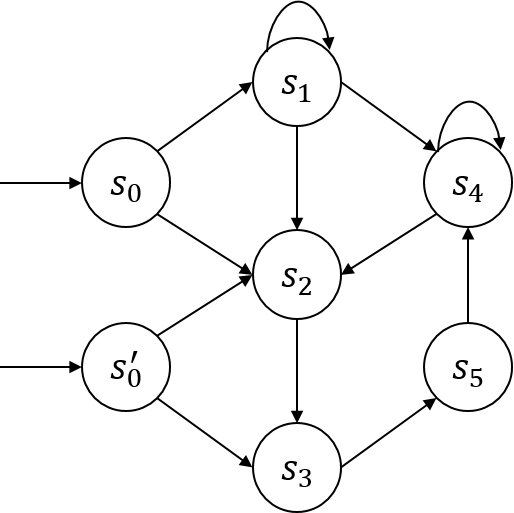
\includegraphics[scale=\figscale]{figures/transition-system.png}
        \caption{Transition system}
        \label{fig:trans-sys}
    \end{subfigure}
    \begin{subfigure}[b]{\subfigw}
        \centering
        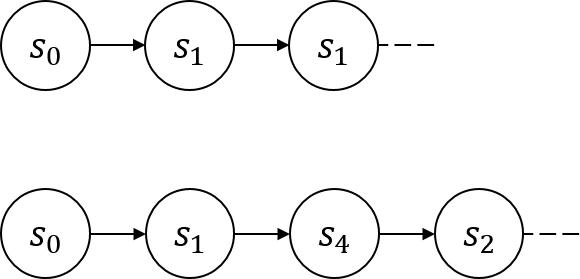
\includegraphics[scale=\figscale]{figures/ltl-interpretation.png}
        \caption{\gls{ltl} interpretation}
        \label{fig:ltl-int}
    \end{subfigure}

    \begin{center}
        \begin{subfigure}[b]{\subfigw}
            \centering
            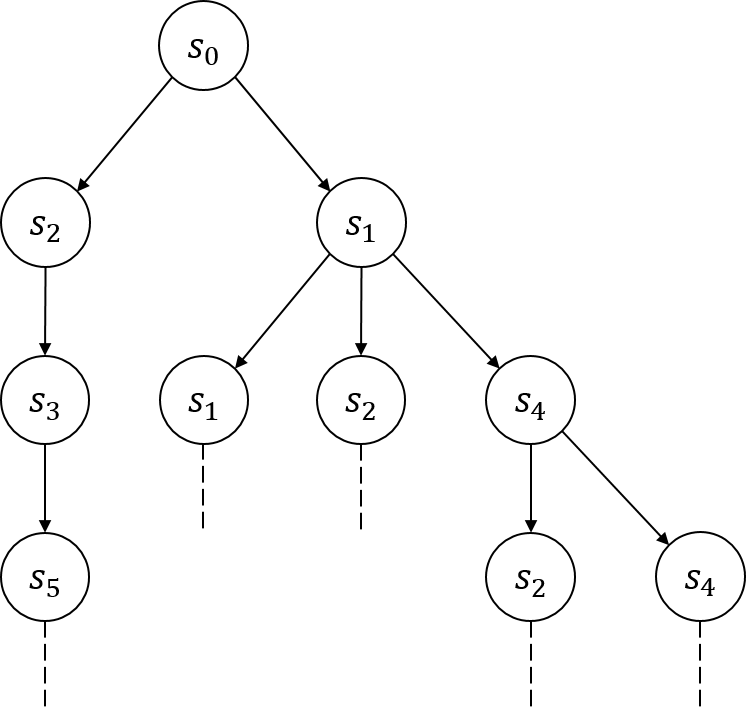
\includegraphics[scale=\figscale]{figures/ctl-interpretation.png}
            \caption{\gls{ctl} interpretation}
            \label{fig:ctl-int}
        \end{subfigure}
    \end{center}
    \caption{nuXmv modules illustrated}
\end{figure}

\gls{ltl}, on the other hand, is a temporal logic and as such supports the specification of properties over time.
Both, \gls{ltl} and \gls{ctl}, will be introduced semi-formally here as presented in the \citetitle{nuXmv} \cite{nuXmv}.
Interpretations and models of an \gls{ltl} formula are infinite execution paths of a state transition system that in context of nuXmv are given by a module.
A state transition system comprises a set of states and a transition relation amongst them with some dedicated initial states.
Such a state can be understood as an assignment to the variables of the nuXmv module that is resembled by the transition system.
An illustration of a transition system is given in figure \ref{fig:trans-sys}.
The transition system comprises two initial states $ s_0 $ and $ s_0' $.
The set of all initial states is given by the set of all assignments satisfying all \smv{INIT} constraints.
Given a state $ s $, the set of its successor states is given by the set of states $ \{ s^+ \mid s $ and $ s^+ $ satisfy all \smv{TRANS} constraints $ \} $.

Such an execution path now is an infinitely long trace of states $ T = (t_1, t_2, \dots) $ such that $ t_1 $ is an initial state, $ t_1 $ and $ t_2 $ satisfy all \smv{TRANS} constraints, etc.
Intuitively, one can understand some execution as a random walk in the transition system starting at an initial state, i.e. some run of the system.
Two example execution paths are depicted in figure \ref{fig:ltl-int}.

The most simple form of an \gls{ltl} formula again is a next-expression \smv{p}.
$ T $ models \smv{p} in \gls{ltl} if \smv{p} is true in $ t_1 $.
Furthermore, there are five main temporal operators.
\gls{ltl} formulas are defined syntactically and semantically in the usual, recursive way where $ \psi, \psi' $ are \gls{ltl} formula:
\begin{description}
    \item[Next] \lstinline[language=smv,mathescape=true]{$ \varphi := $ X $ \psi $}: $ T $ models $ \varphi $ if $ \psi $ is true in $ t_2 $, i.e. $ \psi $ holds in the \textit{next} state.
    \item[Globally] \lstinline[language=smv,mathescape=true]{$ \varphi := $ G $ \psi $}: $ T $ models $ \varphi $ if $ \psi $ is true for \textit{all} $ t_i $, $ 1 \leq i $, i.e. $ \psi $ is \textit{always} true.
    \item[Finally] \lstinline[language=smv,mathescape=true]{$ \varphi := $ F $ \psi $}: $ T $ models $ \varphi $ if $ \psi $ is true for \textit{some} $ t_i $, $ 1 \leq i $, i.e. $ \psi $ is true at \textit{some point} from now on.
    \item[Until] \lstinline[language=smv,mathescape=true]{$ \varphi := \psi $ U $ \psi' $}: $ T $ models $ \varphi $ if $ \psi $ is true in $ t_1 $ to $ t_i $, $ 1 \leq i $, and at $ t_{i + 1} $, $ \psi' $ is true, i.e. $ \psi $ is true \textit{until} $ \psi' $ is true.
    \item[Releases] \lstinline[language=smv,mathescape=true]{$ \varphi := \psi $ V $ \psi' $}: $ T $ models $ \varphi $ if $ \psi' $ holds in $ t_1 $ to $ t_i $, $ 1 \leq i $, and in $ t_i $ also $ \psi $ is true.
    Alternatively, $ i $ might not be bounded, i.e. $ \psi $ then is never and $ \psi' $ globally true.
    This means that $ \psi' $ is true \textit{at least until} $ \psi $ becomes true (which also might be never).
\end{description}

When an \gls{ltl} specification \smv{p} is checked by nuXmv, it is verified that \smv{p} is true for \textit{all} execution paths of the transition system given by the main module.
Consequently, an invariant \smv{p} can also be expressed as the \gls{ltl} formula \smv{G p}.

Additionally, there are analogous operators for the past.
\smv{Y p} and \smv{Z p} are the past-versions of \smv{X} with the distinction that \smv{Y} is false at $ t_1 $ and \smv{Z} is true at $ t_1 $.
The \enquote{Historically} operator \smv{H p} is the counterpart to \smv{G} and the \enquote{Once} operator \smv{O p} is the counterpart to \smv{F}.

\gls{ctl} formulas share much of the idea of \gls{ltl} formulas but they differ in the interpretations and models for formulas.
Whereas in \gls{ltl} an interpretation of a formula is a infinitely long execution path of a transition system, in \gls{ctl} an interpretation of a formula is a transition system itself or more specifically: the unwinded transition relation of a transition system as a tree (hence the name computation \textit{tree} logic).
Therefore, it is straightforward how \gls{ctl} formulas are checked by nuXmv: it is checked whether the transition system unwinded as a tree models the formula.
Consider the example tree depicted in figure \ref{fig:ctl-int}.

Again, the most simple form of a \gls{ctl} formula is a next-expression \smv{p}.
Such a tree $ T $ models \smv{p} if \smv{p} is true in the root state $ s_0 $ of $ T $.
The operators supported by \gls{ctl} are again defined inductively for some \gls{ctl} formula $ \psi $:
\begin{description}
    \item[Exists globally] \lstinline[language=smv,mathescape=true]{$ \varphi := $ EG $ \psi $}: $ T $ models $ \varphi $ if there exists an infinite path $ (s_0, \dots) $ in $ T $ such that $ \psi $ is true for all states on the path.
    \item[Exists next state] \lstinline[language=smv,mathescape=true]{$ \varphi := $ EX $ \psi $}: $ T $ models $ \varphi $ if there exists a direct successor state $ s $ to $ s_0 $ such that $ \psi $ is true in $ s $.
    \item[Exists finally] \lstinline[language=smv,mathescape=true]{$ \varphi := $ EF $ \psi $}: $ T $ models $ \varphi $ if $ \psi $ is true in some successor state $ s $ to $ s_0 $.
    \item[For all globally] \lstinline[language=smv,mathescape=true]{$ \varphi := $ AG $ \psi $}: $ T $ models $ \varphi $ if for all infinite paths $ (s_0, \dots) $ in $ T $, $ \psi $ is true for all states on the respective path.
    \item[For all next state] \lstinline[language=smv,mathescape=true]{$ \varphi := $ AX $ \psi $}: $ T $ models $ \varphi $ if for all direct successor states $ s $ to $ s_0 $, $ \psi $ is true in $ s $.
    \item[For all finally] \lstinline[language=smv,mathescape=true]{$ \varphi := $ AF $ \psi $}: $ T $ models $ \varphi $ if for all infinite paths $ (s_0, \dots) $ there is some $ s $ on the path such that $ \psi $ is true in $ s $.
\end{description}

It can be seen that the most important \gls{ltl} operators \smv{X}, \smv{G} and \smv{F} are adopted to \gls{ctl} by existentially and universally quantifying each.

\begin{example}
    To illustrate the relation of \gls{ltl} and \gls{ctl} consider some module $ M $ and its transition tree $ T $ as well as the set of all execution paths $ P $.
    Now let \smv{p} be some next expression.
    One has:
    \begin{itemize}
        \item $ T $ models \smv{AG p} if and only if for all $ p \in P $, $ p $ models \smv{G p}
        \item $ T $ models \smv{EG} if and only if there exists a $ p \in P $ such that $ p $ models \smv{G p}
    \end{itemize}
    The same applies to \smv{X} and \smv{F} respectively.
    However, in general, \gls{ltl} and \gls{ctl} do not share the same expressive power and neither is strictly more expressive than the other.
\end{example}

\begin{example}
    Consider the example invariant, \gls{ltl} and \gls{ctl} specifications depicted in snippet \ref{snpt:nuxmv-spec}.
    These specify high-level properties about the traffic lights of example \ref{exm:traffic-lights}.

    \begin{figure}
        \begin{lstlisting}[
            language=smv,
            caption={An example of a specification in nuXmv},
            label={snpt:nuxmv-spec}
        ]
            INVARSPEC traffic_lights != ped_lights;
            LTLSPEC G (ped_button -> F ped_lights = g);
            CTLSPEC (AF traffic_lights = g) & (AF ped_lights = g);
        \end{lstlisting}
    \end{figure}


    In nuXmv, specifications are introduced by \smv{INVARSPEC}, \smv{LTLSPEC}, or \smv{LTLSPEC} and optionally may be preceded by a name which is omitted in this example.
    The invariant in this example states that at no point can the traffic and the pedestrian lights show green or red simultaneously.
    The \gls{ltl} formula specifies that whenever the button for the pedestrians is pressed, at some point the pedestrian lights must show green.
    The \gls{ctl} formula specifies that in unwindings of the transition relation, at some point the traffic lights must show green and at some point the pedestrian lights must show green.

    In this example, both the invariant and the \gls{ltl} specification are met by the model.
    The \gls{ctl} specification though is false.
    nuXmv gives the following counter-example:

    \begin{lstlisting}
        -- specification (AF traffic_lights = g & AF ped_lights = g)  is false
        -- as demonstrated by the following execution sequence
        Trace Description: CTL Counterexample
        Trace Type: Counterexample
        -> State: 1.1 <-
        ped_waiting = FALSE
        traffic_lights = g
        ped_lights = r
    \end{lstlisting}

    Counter-examples in nuXmv always show a finite fraction of an infinite execution path.
    For \gls{ltl} formulas, this fraction loops at some point thus inducing an infinite trace.
    For \gls{ctl} formulas on the other hand, the counter-example marks the longest, unambiguous path in the transition tree to a subtree that violates the formula at hand.
    Only one state being depicted in the counter-example above indicates that the computation tree with the initial state given above and in which no variable ever changes violates the \gls{ctl} formula at hand.
    This tree illustrates a world in which the button for pedestrians is never pressed and therefore, the pedestrian lights will correctly never show green.

    While it is not explicitly mentioned in the user manual how input variables relate to the states in the unwinding of the transition relation for the interpretation of a \gls{ctl} formula, it is assumed here that the input variables are not part of the state space; otherwise the counter example given above would not apply since the state where \smv{ped_button} becomes true trivially is reachable.
    This assumption is supported by the fact that in nuXmv, \gls{ctl} formulas must not reference input variables.
    In other words, this means that one must not rely on input variables whilst verifying a system.
\end{example}

\subsection{Summary}

Whereas SPIN was problematic because its input language did not match the needs of this thesis, and SPACER or \muZ{} were problematic because their output does not match the requirements of this thesis, nuXmv fulfills both aspects.
The traces generated as counter-examples serve as illustration what specifically went wrong on a property.
The input language allows to implement modules that are limited in the description of the transition relation itself\footnote{%
    Since transitions are constrained by propositional logic and expressions without loops only, there can be issues if complex transitions should be expressed.
    For example, in section \ref{sec:ifc-model} we will consider a situation where for the transition of a bit vector the first bit that is high needs to be found.
    In other programming languages, one would simply iterate over all bits of the vector and break the loop on the first high bit.
    However, when constraining the transition relation, there are no loops.
    This left us with the need to implement this search for the first high bit as a sequence of nested \smv{( ? : )} expressions resembling the binary search tree for the respective bit.
} but is powerful in expressing modules as a whole.
Having variables and transition allows to implement pretty much any sequential system.
Therefore the decision was made to use nuXmv as a verification engine.

The idea for the implementation is straight-forward:
\begin{itemize}
    \item Use input variables to model instructions to the architecture
    \item Use variables to model the architectural state, i.e. registers, etc.
    \item Use transition constraints to implement the behavior of each instruction
\end{itemize}

We furthermore decided to express the information flow control of the architecture in \gls{ltl}.
nuXmv supports a plethora of techniques to check specifications, e.g., the \citetitle{nuXmv} \cite{nuXmv} lists 47 commands to check a specification.
In the practical work for this thesis, after the decision to implement the \gls{ifc} in \gls{ltl} has been made, a couple of these techniques which apply to \gls{ltl}-checking were tested.
In this informal evaluation it was found that the K-Liveness algorithm proposed in \cite{Claessen12} delivered best results and terminated quickly whenever the model met the specification.
Whenever this was not the case, i.e. the specification was not met by the model which was usually indicated by a long runtime of the K-Liveness algorithm, a \gls{bmc} approach computed counter-examples very efficiently.
As the technique of \gls{bmc} has already been introduced in section \ref{sec:spacer}, now, the key idea behind the K-Liveness algorithm by \citeauthor{Claessen12} shall be investigated.

In \gls{ltl} two types of properties can be distinguished: \textit{safety} and \textit{liveness} properties.
Safety properties are formulas for which every counter example has finite length.
Liveness properties on the other hand can\footnote{%
    Especially, one has that every safety property is also a liveness property but not vice versa.
} have counter-examples which are infinite and cannot be made finite.
The background of the K-Liveness algorithm is that techniques for efficiently solving safety properties already exist, i.e. the IC3 algorithm proposed in \cite{Bradley11}.
\citeauthor{Claessen12} take this algorithm and present a decision procedure for model checking liveness properties on finite state transition systems, i.e. a general algorithm for checking \gls{ltl} formulas on such systems.
The algorithm works on \gls{ltl} formulas of the canonical form: \smv{F G q} where \smv{q} is some \gls{ltl} formula.
The authors implicitly mention that any \gls{ltl} formula $ \varphi $ can be transformed into this form but give no proof or reference for this.
For such properties, \citeauthor{Claessen12} present the following lemma:
\begin{lemma}[\cite{Claessen12}]
    If a state transition system models \smv{F G q}, then there exists some integer $ k $ such that for any trace $ T $, \smv{q} is false at most $ k $ times in $ T $.
\end{lemma}
This leads to a straightforward algorithm that is sound and complete on positive instance of \gls{ltl} formulas:
\begin{enumerate}
    \item Let $ k := 0 $.
    \item Construct a formula \smv{q_new} that encodes: \smv{q} is false at most $ k $ times. \label{itm:k-live-loop}
    This obviously is a safety property.
    \item Consult the IC3 algorithm and check whether \smv{q_new} is true; if it is return that \smv{F G q} is true.
    \item Otherwise; set $ k := k + 1 $ and go to step \ref{itm:k-live-loop}.
\end{enumerate}

To have this algorithm terminate also for negative instances, i.e. where the property at hand is not modelled by the state transition system, the authors complement the basic K-Liveness algorithm with methods dedicated to finding counter-examples.
Such an algorithm needs to construct bounded counter-examples for \smv{q_new}-like properties and detect repeated states in which \smv{q} is false.
If a trace is found where such a state appears at least twice, there also is a trace in which this state occurs infinitely often thus disproving \smv{q} since no $ k $ in accordance to the lemma can be found.

\section{Summary \& Methodology}
\label{sec:sum-background}

The goal of this thesis is to evaluate an approach to formally verifying \glspl{isa} against higher-level information flow properties using a model checker.
This combines the work of \citeauthor{Reid17} \cite{Reid17} and \citeauthor{Ferraiuolo17} \cite{Ferraiuolo17}.
This approach will be evaluated by applying it to a simplified version of the RISC-V \gls{isa}, MINRV8.
We adopt the requirements to these properties from \cite{Reid17}, i.e. these properties should:
\begin{displaycquote}[pp.88:2-3]{Reid17}
    \begin{itemize}
        \item express the major guarantees that programmers depend on;
        \item \textelp{be} concise so that architects can easily review and remember the entire set of properties;
        \item \textelp{be} stable so that architectural extensions do not invalidate large numbers of rules;
        \item \textelp{} describe the architecture differently from existing specification to reduce the risk of common-mode failure.
    \end{itemize}
\end{displaycquote}

To achieve this, we will investigate the RISC-V architecture in more detail and define as well as implement the MINRV8 architecture in chapter \ref{chp:arch}.
This architecture will stick to the \gls{risc}-properties as defined in \cite{Hennessy12} in that it will be a load/store architecture, instructions will operate on registers mainly, and there are few, homogenously encoded instructions available.
A model of this instruction set architecture will be implemented in nuXmv.

As a next step in chapter \ref{chp:ifc}, the terms of an information flow \textit{policy} and information flow \textit{control} will be applied to the MINRV8 architecture, thus, using the work of \citeauthor{Ferraiuolo17} \cite{Ferraiuolo17} to define higher-level properties to verify the architecture against.
Thereby, it will be investigated how the policy in \cite{Ferraiuolo17} which applies to \gls{hdl} code can be carried over to \glspl{isa} and implemented in nuXmv.
By using nuXmv as a verification tool, we enhance on \cite{Reid17} in the key aspect, that unbounded numbers of transitions are taken into account.
When this has been dealt with, the actual \gls{ifc} will be expressed as \gls{ltl} properties.
These properties will assume the user-mode of the system to be compromised and express that insecure flows of information between machine- and user-mode are impossible.

The results of this verification process will be discussed in chapter \ref{chp:results}.
How will these results look like?

The idea of \gls{ifc} is to express properties like: \enquote{Information must not flow like \dots}.
Whenever nuXmv is asked: \enquote{Does this model of the MINRV8 architecture allow for such flows of information?}, it will either respond with yes, giving a sequence of instructions that violate the information flow property, or respond with no.
If the response happens to be a counter-example, the following questions must be investigated:
\begin{enumerate}
    \item \label{itm:counter-ex-validity}
    Is the counter-example legitimate or is it a false positive?
    \item \label{itm:counter-ex-mitigation}
    If the counter-example is legitimate, how can the uncovered vulnerability to the system be mitigated?
\end{enumerate}

The former question arises because the model of the architecture itself might be flawed.
To answer it, one simply must inspect the trace at hand and verify whether all state transitions and variable changes are indeed valid in regard to the specification of MINRV8.
If the answer to this question is no, the implementation has to be fixed accordingly and the proofs must be re-run.

The latter question leads to the actual results.
If it is found that the counter-example at hand is genuine, it must be decided how the newly found vulnerability is handled.
There are two ways to handle a vulnerability.
Either it is a proper architectural vulnerability that must be mitigated accordingly by architectural measures or it shows a vulnerable \textit{usage} of the architecture that cannot be mitigated by the architecture without removing critical features from it.
For example, it is an obvious security issue, when machine-mode directly hands confidential data to user-mode.
No sensible architectural mechanisms could prevent machine mode from doing this as long as machine mode is in fact able to hand data to user mode - which it should be.

In the first case, where it is discovered that a counter-example comprises a proper architectural vulnerability, we will investigate mechanisms that mitigate the respective vulnerability and also attempt to verify the effectiveness of such mitigations by re-running the proofs.
If however, we do not find the counter-example to uncover a vulnerability but rather to describe \textit{vulnerable code}, we will phrase rules to be obeyed by e.g., \gls{os} or compiler engineers that prohibit such bad vulnerabilities.
We also will then verify the effectiveness of these rules by implementing them in the model as assumptions and re-running the proofs as well.

When phrasing assumptions, we impose the following requirements upon them:
\begin{enumerate}
    \item \label{itm:assumptions-non-trivial}
    The assumptions must be non-trivial, i.e. they must not be contradictory and must not trivially entail the information flow properties to be verified,
    \item \label{itm:assumptions-machine-mode}
    the assumptions must only constrain machine-mode, and
    \item \label{itm:assumptions-verifiable}
    the assumptions must be practical and verifiable.
\end{enumerate}

The reasoning behind point \ref{itm:assumptions-non-trivial} is straight-forward:
Working with contradictory assumptions leads to proving \enquote{$ \text{false} \Rightarrow \text{properties} $} which is trivially true.
Likewise, working with assumptions trivially entailing the properties leads to proving \enquote{$ \text{properties} \Rightarrow \text{properties} $} again being trivially true.

Point \ref{itm:assumptions-machine-mode} was raised because it is important to note that the assumptions introduced as a result of this thesis fit in the threat model as discussed in section \ref{sec:threat-model}.
Recall, that in context of this thesis it is assumed that user-mode is adversarial to machine-mode and compromised completely.
Constraining user-mode in the assumptions therefore would have contradicted this threat model.

Lastly, we hope that the assumptions established in context of this thesis can serve as a verification target for \glspl{os} or compilers.
This is expressed in point \ref{itm:assumptions-verifiable}.
If one was to write a collection of interrupt handlers for an \gls{os}, these assumptions might be used to verify that each rule given by these assumptions is implemented by handlers.
This would grant the absence of information flow related bugs in context of the information flow properties as proposed in section \ref{sec:ifc-properties}.
This, however, presupposes that it is actually possible to verify programs against these properties.
As part of this thesis, we cannot give guarantees on the feasibility of this undertaking.
Yet, we try to allow for it.

These steps constitute an interactive prove-refine loop that is depicted in figure \ref{fig:ver-process}.
This loop is entered by running nuXmv in order to prove the absence of any \gls{ifc} violations.
If, however, there is such a violation, the model will be refined either by a fix or by a refinement of the architecture or by a refinement of the assumptions implementing rules to secure usage of the architecture.
At some point, a set of respective fixes, architectural changes and assumptions will mark a fixpoint to this loop where no further refinement is necessary and finally, no \gls{ifc} violations can be found.

\begin{figure}
    \centering
    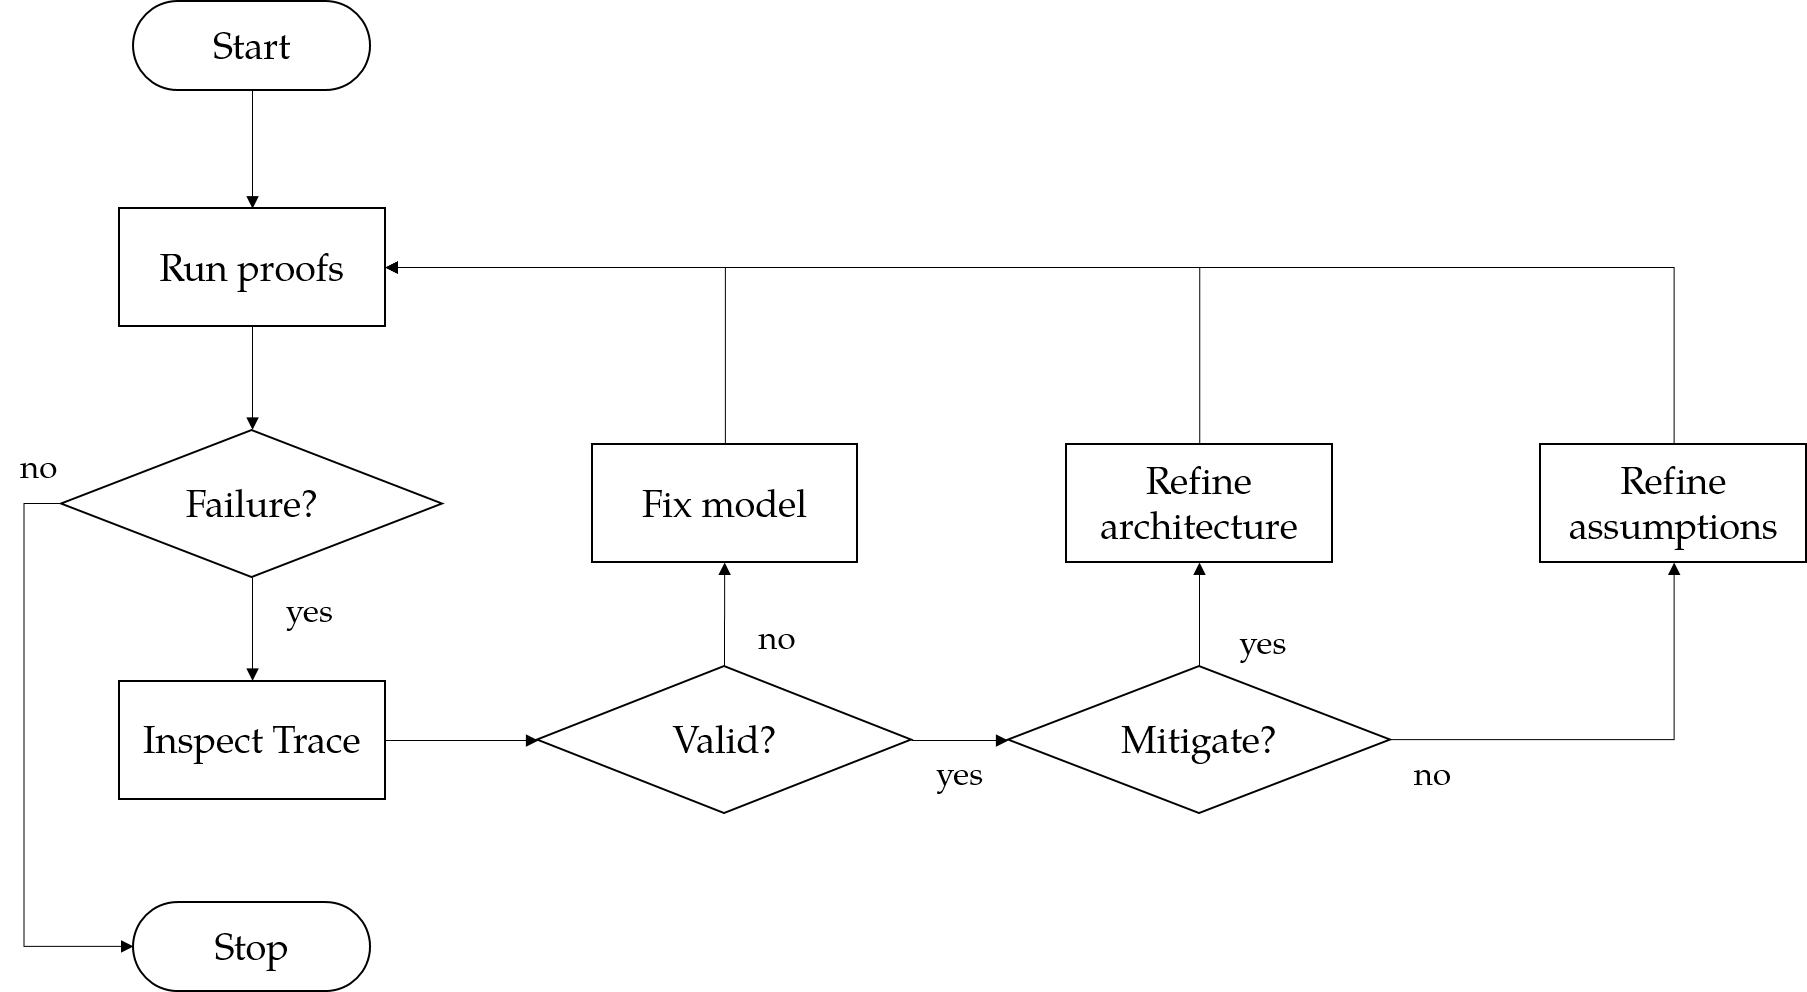
\includegraphics[width=\textwidth]{figures/verfification-process.png}
    \caption{Verification Process Flowchart}
    \label{fig:ver-process}
\end{figure}

This is what will be presented in chapter \ref{chp:results}.
From chapter \ref{chp:discussion} onwards, these results will be discussed, put into context of related work in chapter \ref{chp:related-work} and finally summarized in chapter \ref{chp:conclusion}.

%!TEX root = ../thesis.tex

\section{Architecture}
\label{sec:arch}

\subsection{An Introduction to RISC-V}

This section will introduce the core of the \gls{riscv} architecture by shedding light on the base integer instruction set in section \ref{sec:rv-base-int-isa} and the mechanisms of the privileged part of the architecture in \ref{sec:rv-priv-arch}.

\subsubsection{The Base Integer Instruction Set}
\label{sec:rv-base-int-isa}

\paragraph{Instructions}

\subparagraph{Integer arithmetic and Boolean instructions}
The base integer instruction set provides instructions for plus and minus, integer comparisons and the Boolean operators \rv{And}, \rv{Or} and \rv{Xor}.
Most of these instructions are implemented in two version: a register version (or R-type instruction) and an immediate version (or I-type instruction).
In the first case the two operands are given as registers and in the second case one operand is given as register and the other as an immediate value read from memory.
In either case the value is stored in a destination register.

These basic instructions are all side effect free besides from advancing the program counter which means that if the destination register is x0, each of them encodes a no-operation instruction.
This makes them particularly easy to analyze.
However, as a side-effect, this means that there is no built-in support for overflow checks via flags in some dedicated \gls{csr}.
There also is no special instruction to handle this.
The authors of the \gls{riscv} manual show that in general, overflow checks for addition can be handled with three additional instructions after an add instruction:

\begin{lstlisting}[
    language=rv,
    caption={General overflow checking \cite{RiscVISA}},
    label={snpt:rv-overflow}
]
    Add  t0, t1, t2          # Set R[t0] to R[t1] + R[t2]
    Slti t3, t2, 0           # Set R[t3] to R[t2] < 0
    Slt  t4, t0, t1          # Set R[t4] to R[t0] < R[t1]
    Bne  t3, t4, overflow    # If R[t3] != R[t4] branch to overflow
\end{lstlisting}

The gist of snippet \ref{snpt:rv-overflow} boils down to: we can check if there was overflow when calculating $ a + b $ by checking whether $ b < 0 \leftrightarrow a + b < a $ is false, i.e. \textcquote{RiscVISA}{the sum should be less than one of the operands if and only if the other operand is negative}.

\subparagraph{Memory operations}
There are two types of instructions that deal with external memory.
Firstly, simple load and store instructions that read from or write to memory.
Secondly, FENCE instructions that synchronize memory access between multiple \glspl{hart}.

Memory in \gls{riscv} is byte-addressable.
Therefore, load and store operations in \gls{riscv} can read or write words of size 8-, 16-, 32-, 64- or 128-bits, depending on the maximum word length of the base instruction set of choice.
Read- and write-addresses don't have to be aligned by software before using them, however, if they are not, the architecture must first align them before fetching from or storing to them, i.e. reading a 32-bit word from memory at address 0x1 is impossible.
If this address is given as argument to a respective load instruction it'll be aligned to the address 0x0.

\subparagraph{Control transfer instructions}
There are two types of instructions that can control program flow in \gls{riscv}: jumps and branches.
In short, jumps are performed unconditionally and can target a wider range in memory (at least $ \pm 2^{20}\text{bits} $ in case of a 32-bit architecture) whereas branches are performed conditionally, only can target a narrower range in memory ($ \pm 2^{12}\text{bits} $ in case of a 32-bit architecture) and always must branch to \gls{pc}-relative addresses.

In contrast to memory operations, addresses targeted by jumps must be aligned correctly.
If this is not the case, an exception will be generated.

Jumps are intended to call routines and functions.
This is why they store a return address to some general purpose register.
Branches on the other hand are intended to control the program flow of one such routine or function, e.g. to implement an \textit{if-else} structure or \textit{for}-loops where code won't return from the branched execution.
\gls{riscv} is agnostic about the details of calling conventions for routines, e.g. how the stack is organized, which general purpose registers are used as \gls{lr} or \gls{sp}, and leaves these details to be implemented by software running on the core.

\subparagraph{Platform management instructions}
The last type of instructions to be looked at are platform management instructions.
The \gls{riscv} manual also knows this category and divides it into two subcategories: instructions that deal with \glspl{csr} and other instructions that perform operations that potentially need some form of privilege.
Examples for the former category are straight forward.
\gls{riscv} knows instructions to read or write complete \glspl{csr} but also knows operations to modify single bits only.
For the latter category, \gls{riscv} only knows two instructions at the base instruction set level which are \gls{ecall} and \gls{ebreak} instructions.
We will inspect these instructions in more detail in section \ref{sec:rv-priv-arch}.

\subparagraph{Summary}
The base integer instruction set of \gls{riscv} gives you everything you need for implementing a comfortable Turing-machine but pretty much nothing more.
You can perform basic arithmetic with integers or bit vectors of Booleans, load and store results of your calculations and abstract your code by using jumps and branches.
At this point, there is no state with predefined semantics, i.e. all state available is given by storage that can only influence computation when used by a programmer.

Only the platform management instructions give a hint on the complexity that is offered by the \gls{riscv} architecture to allow abstracting processing done on the core.

\subsubsection{The Privileged Architecture}
\label{sec:rv-priv-arch}

The \textit{The RISC-V Instruction Set Manual, Volume II: Privileged Architecture} \cite{RiscVISAP} mainly specifies three concepts:
\begin{enumerate}
    \item Three levels of privilege
    \item Exceptions, traps and interrupts
    \item Memory attributes
\end{enumerate}

The three levels of privilege form the basis of everything that is defined by the privileged architecture.
The purpose of interrupts and exceptions is not only to handle error conditions that arise during runtime but also to communicate between privilege layers.
Therefore, interrupts and exceptions are being used by up to this point unmentioned auxiliary mechanisms of the architecture that aid the highest privilege in administrating the platform.

Also, memory attributes rely on these levels of privilege as they define which mode is eligible to do some operation on some region of memory.

In this section, the aforementioned concepts will be introduced subsequently and will be concluded by a sketch of the auxiliary mechanisms that build on top of these.

\paragraph{Levels of Privilege}

\gls{riscv} knows three privilege levels: user-mode, supervisor-mode and machine-mode\footnote{%
    In an earlier version, there was a fourth privilege-mode being hypervisor-mode that was more privileged than supervisor- but less privileged than machine-mode.
    However, this mode has been dropped from the specification as of now.
    Yet, \gls{riscv} still needs to encode mode-relative bit-fields with two bits.
    Usually, 00 stands for user-, 01 for supervisor and 11 for machine-mode.
    10 is reserved in most places and has been used for hypervisor-mode.
}.
Each implementation of the \gls{riscv} specification must at least provide machine-mode as a base mode of operation.
Besides this, there are two other choices of privilege levels combinations supported:
\begin{enumerate}
    \item Machine-mode only (\textcquote{RiscVISA}{simple embedded system})
    \item User and machine-mode (\textcquote{RiscVISA}{secure embedded system})
    \item User, supervisor and machine-mode (\textcquote{RiscVISA}{\textins{system} running Unix-like operating systems})
\end{enumerate}

A visualization of these three combinations is given in figure \ref{fig:rv-priv-lvls} where they are depicted from left to right.
A simple embedded system might be the cheapest to implement and manufacture, however, this system lacks any protection against malicious application code, i.e. one would only want to run such a system in very basic scenarios where full control over all source code and the device itself can be guaranteed.

A secure embedded system supports some application to be run on it while an \gls{aee} running in machine-mode controls the execution of this application.
The application communicates to the \gls{aee} via an \gls{abi} that defines the possible interactions between an application and an \gls{aee}.

A system running a Unix-like \gls{os} enhances on this by having an \gls{os} running in supervisor-mode that communicates with multiple applications running in parallel via an \gls{abi} and itself is managed by a \gls{see} which communicates with the \gls{os} via a \gls{sbi}.
The \gls{see} runs in machine-mode.

\begin{figure}
    \centering
    \subcaptionbox{\centering Simple embedded system}
    [0.18\textwidth]{
        \begin{tabular}{| c |}
            \hline
            Application \\ \hline
        \end{tabular}
    }
    \quad
    \subcaptionbox{\centering Secure embedded system}
    [0.18\textwidth]{
        \begin{tabular}{|c|}
            \hline
            Application \\ \hline
            \cellcolor{black} \textcolor{white}{ABI} \\ \hline
            AEE \\ \hline
        \end{tabular}
    }
    \quad
    \subcaptionbox{\centering System with Unix-like OS}
    {
        \begin{tabular}{| c | c | c |}
            \cline{1-1} \cline{3-3}
            Application & \multirow{2}{*}{\dots} & Application \\
            \cline{1-1} \cline{3-3}
            \cellcolor{black} \textcolor{white}{ABI} & & \cellcolor{black} \textcolor{white}{ABI} \\ \hline
            \multicolumn{3}{| c |}{OS} \\ \hline
            \multicolumn{3}{| c |}{\cellcolor{black} \textcolor{white}{SBI}} \\ \hline
            \multicolumn{3}{| c |}{SEE} \\ \hline
        \end{tabular}
    }
    \caption{Privilege level combinations \cite{RiscVISA}}
    \label{fig:rv-priv-lvls}
\end{figure}

To keep things simple, the focus of this thesis lies on secure embedded systems\footnote{%
    % TODO: But will it?
    This will be justified in more detail in section \ref{sec:minrv8} where we introduce the architecture that will be verified as part of this thesis.
}.
This means that the architecture to be worked with supports two modes: user- and machine-mode.
Machine-, user- and supervisor-mode do not simply form a linear order of privilege attributes of code execution.
They differ in the concepts that are available to them and therefore must be handled separately.
However, as the focus will lie on secure embedded systems, many parts of the specification which are about supervisor solely will be left out.
Supervisor-mode will be handled wherever it fits in the bigger picture but not on its own.

\paragraph{Exceptions, traps and interrupts}
\label{sec:rv-exn}

Volume 1 of the \gls{riscv} specification \cite{RiscVISA} introduces the concept of exceptions, traps and interrupts as follows:
\begin{displaycquote}{RiscVISA}
    We use the term \textit{exception} to refer to an unusual condition occurring at run time associated with an instruction in the current RISC-V thread.
    We use the term \textit{trap} to refer to the synchronous transfer of control to a trap handler caused by an exceptional condition occurring within a RISC-V thread.
    Trap handlers usually execute in a more privileged environment.

    We use the term \textit{interrupt} to refer to an external event that occurs asynchronously to the current RISC-V thread.
    When an interrupt that must be serviced occurs, some instruction is selected to receive an interrupt exception and subsequently experiences a trap.

    The instruction descriptions in following chapters describe conditions that raise an exception during execution.
    Whether and how these are converted into traps is dependent on the execution environment, though the expectation is that most environments will take a \textit{precise} trap when an exception is signaled \textelp{}.
\end{displaycquote}

This - in short - means that a trigger for interrupts, traps and exceptions can be given which is depicted in figure \ref{fig:trigger-hierarch}.
In general, interrupts occur asynchronously and trigger synchronous exceptions to be generated for a \gls{hart} which in turn may generate traps but also might be handled otherwise.
The specification mentions the example of the floating-point extension in which exceptions not necessarily generate traps.

\begin{figure}
    \centering
    \tikz \graph[grow right sep] {
        Interrupt -> Exception -> {Trap, ?};
    };
    \caption{Trap-Trigger-Hierarchy}
    \label{fig:trigger-hierarch}
\end{figure}

For the sake of simplicity, we will assume that every exception causes a trap.
As we will not implement any floating-point arithmetic extension, the specification does not demand from us to handle exceptions otherwise and doing so does not serve any purpose at this point.
In following paragraphs, an introduction to the control flow of dealing with interrupts will be given.
Said control flow is depicted in figure \ref{fig:interrupt-handling} and follows these general steps:
\begin{enumerate}
    \item If an interrupt or exception is pending, determine the privilege mode to take the trap
    \item Check if the interrupt is enabled
    \item Take the trap
    \item Return from trap handler
\end{enumerate}
Interrupt handling can be understood as a generalized form of exception handling as exception handling in principle works the same but has fewer steps.

\begin{figure}
    \centering
    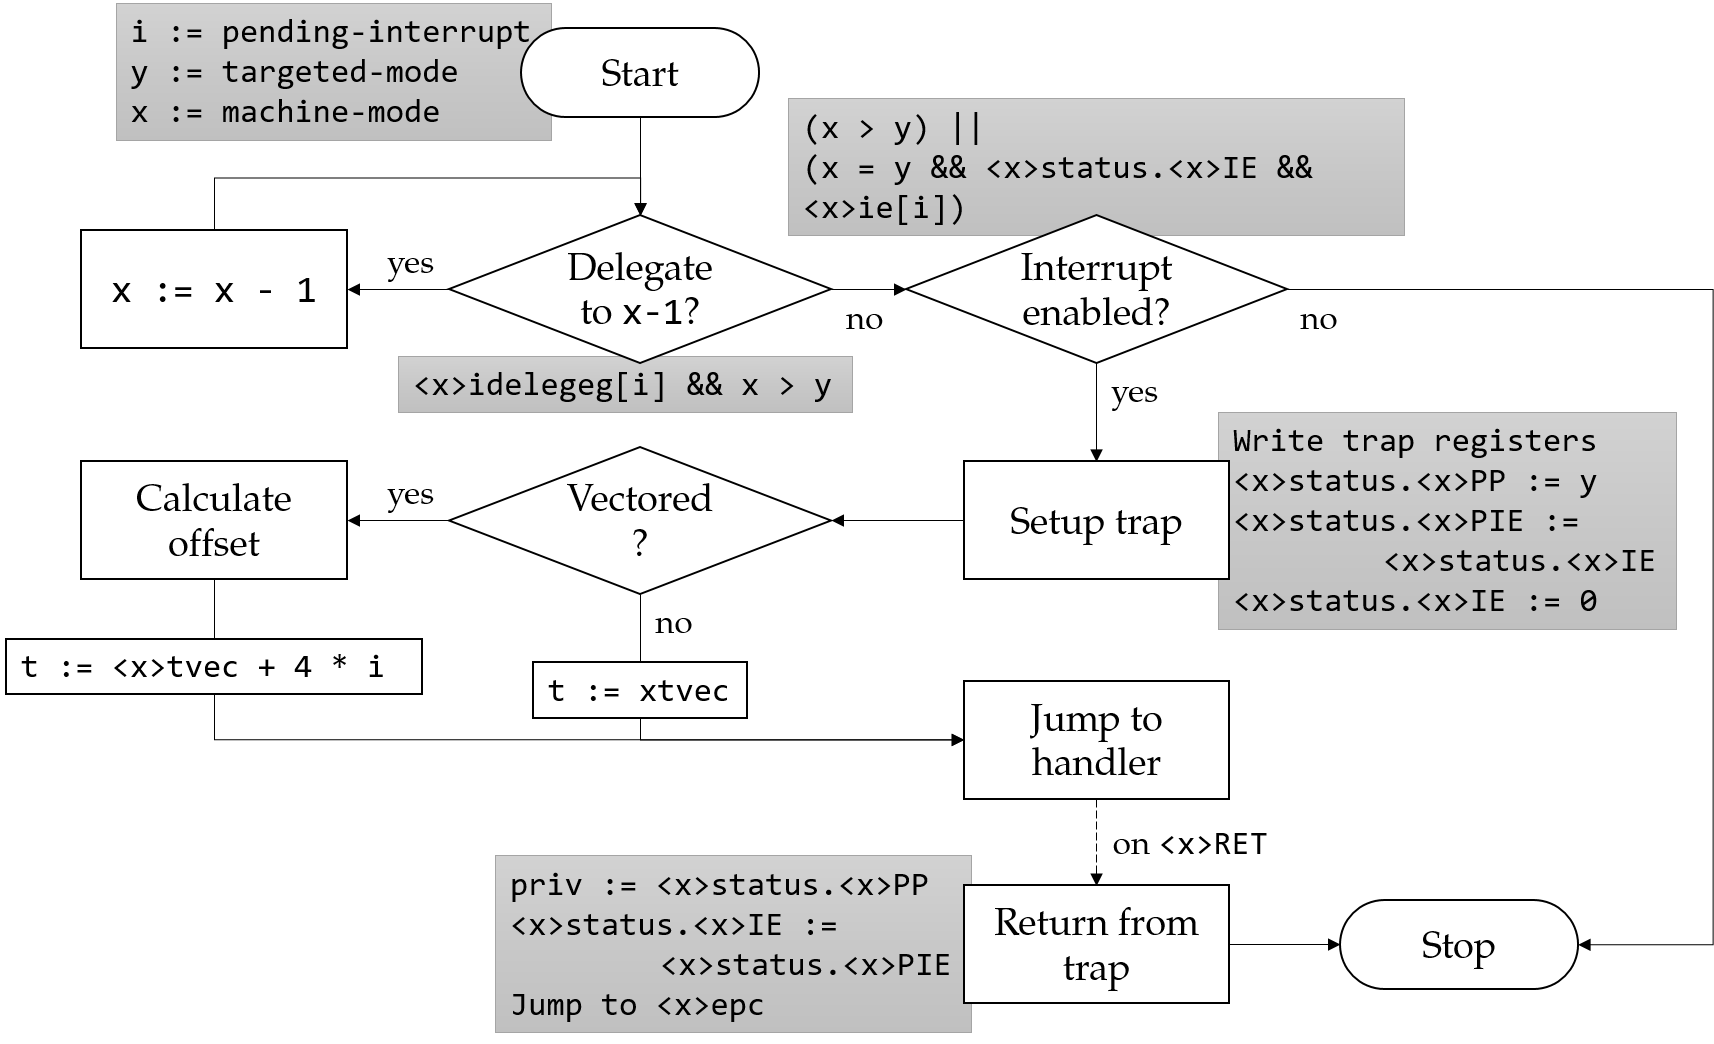
\includegraphics[width=\textwidth]{figures/interrupt-handling.png}
    \caption{Interrupt handling flow-chart}
    \label{fig:interrupt-handling}
\end{figure}

\subparagraph{Interrupt and exception handling}
There are three categories of interrupts: external interrupts, timer interrupts and software interrupts.
External interrupts are used to signal exceptional events occurring on some external device that is connected to the core.
Timer interrupts can be used to track time.
Code can use certain \glspl{csr} to signal to the platform that it needs to be alerted when a given amount of real world time has passed.
Such an alert will be given by a timer interrupt.
More on this in section \ref{sec:other-mechs}.
Software interrupts can be set pending by software running on the same \gls{hart} with equal or higher privilege than the targeted privilege mode.
Software interrupts have no predefined semantics and thus can be used by programmers or system designers in every imaginable way.

Each of these categories of interrupts can target any privilege-mode netting a total of 6 interrupts available to the platform in our case (or 9 if supervisor-mode is supported).
These interrupt-types are associated with indices in the range from $ 0_{10} $ to $ 11_{10} $, also called interrupt code\footnote{%
    The reader might have noticed that these are more indices than needed to encode all interrupts available - even if supervisor-mode is present.
    Indices 2, 6 and 10 currently are reserved because hypervisor-mode has been dropped.
    The two least significant bits of the interrupt indices' encoding correspond to the respective mode's encoding.
    Thus 2, 6 and 10 are reserved as their two least significant bits are $ 10_2 $ corresponding to hypervisor-mode.
}.
An overview of all interrupt codes can be found in table \ref{tbl:interrupt-exception-codes}.
Interrupts can be set pending individually in the \gls{mip} register.
An interrupt is set pending if the bit of the \gls{mip} corresponding to the interrupts index is set to 1.

If an interrupt or exception is set pending, it must first be decided which privilege mode will take the trap to handle the exception generated.
By default, all interrupts and exceptions will be handled by machine-mode.
However, interrupts and exceptions can be delegated to less privileged modes via the \gls{mideleg} and \gls{medeleg} register\footnote{%
    It would also be possible to delegate traps by using the \gls{mret} instruction and setting all corresponding \glspl{csr} accordingly.
    However, this would come with a higher latency as a couple of jumps would need to be performed first.
}.
Similar to \gls{mip} and \gls{mie}, each bit field of \gls{mideleg} corresponds to the interrupt of the same index.
Exceptions also have an exception code assigned and thus, fields of \gls{medeleg} correspond to these codes.
An interrupt or exception can only be delegated to modes equally or higher privileged than the mode the interrupt or exception was targeting originally for example, if an interrupt is targeting supervisor-mode it must be handled by machine-mode or can optionally be delegated to supervisor-mode but can not be handled by user-mode.
If an interrupt is delegated to mode $ x $ ($ x \in \{ \text{M}, \text{S}, \text{U}\} $\footnote{%
In future, we will simply use $ x $ or other variables as placeholders for a mode-flag without specifically introducing the variable.
}), the corresponding bit in $ x\text{ip} $ reads accordingly and $ x\text{ie} $ becomes writable.
Otherwise both registers appear to be hardwired to zero.

After the mode to be targeted by the trap has been determined, it must be checked whether the given interrupt is actually enabled.
Exceptions can't be disabled and therefore will always be taken - as a consequence the following checks will be omitted for exceptions.
Interrupts on the other hand can be dis- or enabled individually in the \gls{mie} register.
Analogously to the \gls{mip} register, an interrupt is enabled if the bit corresponding the interrupts index is set to 1.
Additionally, there is the \gls{mstatus} register which can globally dis- or enable interrupt handling for a specific mode via its $ x\text{IE} $ bits.
The \gls{ustatus} register only is a restricted view on \gls{mstatus} and therefore \gls{mstatus} holds these bits not only for machine- but any mode.
These $ x\text{IE} $ fields, however, are only taken into account if the \gls{hart} operates at an equal or higher privilege mode than targeted, i.e. interrupts are always enabled globally it is targeting a mode of higher privilege than the mode of current operation.
Finally, an interrupt will be taken if interrupts are globally enabled \textit{and} the interrupt itself is enabled in the \gls{mie} register.

If a pending interrupt is taken, the \gls{mepc}, \gls{mcause} and \gls{mtval} registers are written and the platform will jump to a base address held by the \gls{mtvec} register.
\gls{mtvec} also provides a field that controls whether interrupts can be \textit{vectored}, i.e. for interrupts the \gls{pc} is not set to the base address for handling trap but to $ (\text{base} + 4 \times \text{cause}) $.
\gls{mepc} holds the address of the original instruction stream that was preempted, i.e. either the address of the instruction that caused the exception or the instruction that was next to be executed as a external interrupt was taken.
\gls{mcause} holds an identifier of the current interrupt or exception being handled by the trap.
The most significant bit indicates whether an interrupt is currently being serviced and all other bits hold the exception or interrupt code.
\gls{mtval} serves as a register to hold arguments for a trap handler.
Technically, it holds \textcquote{RiscVISAP}{exception-specific information to assist software in handling the trap}.
One example for such \enquote{exception-specific information} is that \gls{mtval} can contain the faulting bits of an instruction for an illegal instruction exception whereas \gls{mepc} would only point to the instruction in memory as a whole therefore not giving specific information about which part of the instruction caused the exception.

\gls{mstatus} also provides bits to \enquote{stack} certain values when handling exceptions or interrupts.
Nested interrupts are only supported between privilege modes.
On a trap to handle an interrupt in mode $ x $, interrupts are disabled for this mode and the value of the interrupt-enable bit is \enquote{stacked onto} a prior-interrupt-enable bit $x\text{PIE} $, i.e. $ x\text{PIE} := x\text{IE} $ and $ x\text{IE} := 0 $.
Additionally, there is a prior-privilege bit $ x\text{PP} $ that stores the privilege mode before the trap was taken.

% TODO: Maybe exactly one instruction? How does alignment play into this?
Note that due to the small offset between vectored interrupt jump destinations, the instructions located there can't perform much more than jumping to the \textit{real} trap handler.
Furthermore, as exceptions can't be vectored, any differentiation between those must be performed by software.

\begin{table}
    \centering
    \begin{tabular}{| r | r | l |}
        \hline
        Interrupt & Exception Code & Description \\
        \hline
        1 & 0 & User software interrupt \\
        1 & 1 & Supervisor software interrupt \\
        1 & 2 & \textit{Reserved} \\
        1 & 3 & Machine software interrupt \\
        \hline
        1 & 4 & User timer interrupt \\
        1 & 5 & Supervisor timer interrupt \\
        1 & 6 & \textit{Reserved} \\
        1 & 7 & Machine timer interrupt \\
        \hline
        1 & 8 & User external interrupt \\
        1 & 9 & Supervisor external interrupt \\
        1 & 10 & \textit{Reserved} \\
        1 & 11 & Machine external interrupt \\
        \hline
        1 & $ \geq $ 12 & \textit{Reserved} \\
        \hline
        0 & 0 & Instruction address misaligned \\
        0 & 1 & Instruction access fault \\
        0 & 2 & Illegal instruction \\
        0 & 3 & Breakpoint \\
        0 & 4 & Load address misaligned \\
        0 & 5 & Load access fault \\
        0 & 6 & Store \textelp{} address misaligned \\
        0 & 7 & Store \textelp{} access fault \\
        0 & 8 & Environment call from U-mode \\
        0 & 9 & Environment call from S-mode \\
        0 & 10 & \textit{Reserved} \\
        0 & 11 & Environment call from M-mode \\
        0 & 12 & Instruction page fault \\
        0 & 13 & Load page fault \\
        0 & 14 & \textit{Reserved} \\
        0 & 15 & Store \textelp{} page fault \\
        0 & $ \geq $ 16 & \textit{Reserved} \\
        \hline
    \end{tabular}
    \caption{Interrupt and exception codes \cite{RiscVISAP}}
    \label{tbl:interrupt-exception-codes}
\end{table}

\subparagraph{Summary}
You can find an overview over all registers that are involved in trap handling in table \ref{tbl:trap-csrs}.
Those \glspl{csr} which are available to user-mode would also be available to supervisor-mode in this context.
Registers written in italic font are not actual registers on their own but provide a restricted view on their respective machine-mode counterpart.

\begin{table}
    \centering
    \begin{tabular}{| c c || l |}
        \hline
        \textbf{Machine-mode} & \textbf{User-mode} & \textbf{Description} \\
        \acrshort{mstatus} & \textit{\acrshort{ustatus}} & Status \\
        \acrshort{mie} & \textit{\acrshort{uie}} & Interrupt enable \\
        \acrshort{mip} & \textit{\acrshort{uip}} & Interrupt pending \\
        \acrshort{mtvec} & \acrshort{utvec} & Trap-vector base address \\
        \acrshort{mscratch} & \acrshort{uscratch} & Scratch \\
        \acrshort{mepc} & \acrshort{uepc} & Exception program counter \\
        \acrshort{mcause} & \acrshort{ucause} & Trap cause \\
        \acrshort{mtval} & \acrshort{utval} & Trap value \\
        \acrshort{medeleg} & & Exception delegation \\
        \acrshort{mideleg} & & Interrupt delegation \\
        \hline
    \end{tabular}
    \caption{Trap-handling \glspl{csr}}
    \label{tbl:trap-csrs}
\end{table}

To summarize the mechanisms that play into interrupt and exception handling, recall the four steps to interrupt and exception handling we introduced at the beginning of this section.
These can now be filled with more details:
\begin{enumerate}
    \item If an interrupt or exception is pending, determine the privilege mode to take the trap by checking the targeted privilege mode and any delegation settings
    \item If an interrupt is pending, check that interrupts are enabled globally and the specific interrupt is enabled as well
    \item Take the trap by jumping to to trap base vector and if an interrupt is being serviced take vectoring into account
    \item Return from trap handler
\end{enumerate}

The differences between handling exceptions and interrupts can be summarized by the following:
\begin{itemize}
    \item Exception can't be disabled therefore they will always be handled
    \item $ x\text{cause}[31] $ is written with $ 0 $
    \item Exceptions can't be vectored therefore the \gls{pc} will always be set to $ x\text{tvec} $
\end{itemize}

One would need to alter figure \ref{fig:interrupt-handling} by replacing most interrupt-related \glspl{csr} with their exception-related counterpart if possible.
An exception to this is $ x\text{status}.x\text{IE} $ which still is set to 0 meaning that it is not possible to preempt handling an exception by handling an interrupt.

Finally, note that exceptions are handled as soon as they occur.
This is necessary as exceptions always are closely related to the current stream of instructions and therefore need attention before said stream can continue to be executed.
The only exception to this are other interrupts which are handled before any exception with the following decreasing order of priority: external interrupts, software interrupts, timer interrupts, exceptions.
% Source: https://stackoverflow.com/a/56402079/7194995
\gls{riscv} knows no concept of settings exceptions pending, this however, isn't necessary.
If an exception occurs while an interrupt is set pending, the interrupt can be handled with \gls{mepc} being set to the address of the faulting instruction which either will again fault after the interrupt has been handled or will succeed by some magical condition in which case it does need any further attention.

% TODO: Mention what I didn't mention; e.g. specific parts of mstatus

\paragraph{Memory Attributes}
\label{sec:memory-attrs}

In the previous paragraph, it was mentioned that \gls{mstatus} contains some bits that are not directly relevant to trap handling.
In this section, these bits will be introduced alongside another \gls{csr} that is related to trap handling.

These two remaining fields of \gls{mstatus} deal with memory privilege translation for machine-mode.
Firstly, there is the MPRV bit which can translate memory access privilege.
This bit is only available if at least two privilege modes are supported otherwise it is hardwired to zero.
If MPRV is set to one, \textcquote{RiscVISAP}{load and store memory addresses are translated and protected as though the current privilege mode were set to MPP}, i.e. they're performed with the privilege level that has was preempted by taking the trap.
Secondly, there is the MXR field that allows to read executable memory regions.
If MXR is not set, attempting to read from a memory region marked as executable will fail.
If MXR is set, such reads can succeed if said region is also marked as readable.
% TODO: is page-based virtual memory given?
MXR is only applicable though, if page-based virtual memory is in place.

The last register we will introduce is the \gls{mscratch} register which can be used by machine-mode to be read from and written to for preserving any value the machine-mode would like to see preserved.
The intended use-case for this register by the specification is that \textcquote{RiscVISAP}{it is used to hold a pointer to a machine-mode \gls{hart}-local context space and swapped with a user register upon entry to a \textins{machine}-mode trap handler}.

% TODO: Introduce pma- and pmpcfg

\paragraph{Other Mechanisms}
\label{sec:other-mechs}

\subparagraph{Timer and performance counter \glspl{csr}}
There also is a group of registers dealing with timers and hardware performance monitoring, namely: \gls{mtime}, \gls{mtimecmp}, \gls{mcycle}, \gls{minstret}, \gls{mhpmcountern}, \gls{mhpmeventn} and \gls{mcounteren}.
Details on these registers will be skipped here as these registers also won't be part of this thesis.
The reasoning for skipping these is not as straight-forward as for the previously introduced registers.
In general, timer and performance counting registers can be used for side channel attacks.
In \cite{Qian16} the authors give an overview over timing-side-channel-attacks which by their very nature always need to rely on some notion of time.
This notion can be given by timer and performance counter registers which for example hold the number of instructions executed since a given point in time.
For example, the authors discuss an attack where a side channel to OpenSSL's implementation of \gls{rsa} could be introduced by differentiating between multiplications and squares being performed.
Such a differentiation could be easily done if performance counter registers where to count such instructions and were to leak information to lower privilege levels.
This means that in principle, timer and performance counter registers are relevant for the security of an architecture.
However, they do not introduce new notions of information flow to the architecture and are therefore redundant to our thesis.

It is the case that contents of these registers are confidential as their contents might be used to introduce side-channels to other applications running on the processor.
However, their core mechanisms are not unique.
They can be read and written to and might generate interrupts.
Therefore, dealing with information flow in general is sufficient for our approach and these registers can be safely ignored without loosing major aspects of the \gls{riscv} functionality.

Besides the interrupts and exceptions that have been introduced in the last few paragraphs, there are two further \textit{exceptional conditions} that can occur in a \gls{hart}.

\subparagraph{Reset}
The first of these is the reset.
The specification does not explicitly define how resets are triggered but it is clear that at least hardware must be capable of triggering a reset, e.g. by the push of a button that is on a shared board with the processor.
As the specification gave an exhaustive list of exceptions and interrupts available to the system (which is given in table \ref{tbl:interrupt-exception-codes}), it is assumed here that resets can be triggered by hardware only.

On reset, the \gls{pc} is set to an implementation defined address, the privilege mode is set to machine-mode, the MIE and MPRV bits in \gls{mstatus} are set to 0 and \gls{mcause} should be written with implementation-defined values to indicate the cause of the reset.
The specification explicitly mentions that \textcquote{RiscVISAP}{%
    \textins{a}ll other hart state is undefined
} although software located at the reset vector might write \glspl{csr} with arbitrary values.

% Source: https://stackoverflow.com/a/46989066/7194995
Although the specification itself says that the \textcquote{RiscVISAP}{\texttt{pc} is set to an implementation-defined reset vector} and does not lay any constraints on this, this address must not be the same as \gls{mtvec}.
The reason for this is given in a comment to this section where it says:
\begin{displaycquote}{RiscVISAP}
    \texttt{mcause} reset values may alias \texttt{mcause} values following synchronous exceptions.
    There is no ambiguity in this overlap, since on reset the \texttt{pc} is set to a different value than on other traps.
\end{displaycquote}

Although comments should not be taken with the same weight as regular passages of the specification, the intent behind this comment is quite clear and as it only slightly contradicts the specification we will go with this interpretation.

\subparagraph{Non-Maskable Interrupts}
The other exceptional condition are \glspl{nmi}.
The specification describes these as: \textcquote{RiscVISAP}{%
    \textins{NMIs} are only used for hardware error conditions, and cause an immediate jump to an implementation-defined NMI vector running in M-mode regardless of the state of a hart's interrupt enable bits.
}
Similar to resets, nothing is said about the mechanisms to trigger \glspl{nmi} in the specification.
For the same reasons given in the paragraph about reset, we will assume that \glspl{nmi} can only be triggered by hardware.

On jump to the \gls{nmi} handler address, \gls{mepc} is written with the next address to be read and executed and \gls{mcause} is written with information about the cause of the \gls{nmi}.
Other \glspl{csr} are left untouched.

% TODO: Summarize

% TODO: Add goal of the architecture and in particular, checking it

\subsection{The MINRV8 Architecture}
\label{sec:minrv8}

The architecture that will be model checked in this thesis is a minimal, \gls{riscv}-inspired 8-bit architecture and shall be named MINRV8 from now on.
A secure embedded system that implements the RV32E, i.e. base integer instruction set for embedded computing, was taken as a role model for this minimal architecture.

MINRV8 supports 4 general purpose registers and has two privilege modes: machine- and user-mode.
Besides this, it has 4-bytes of readable and writeable memory which is divided into two regions the first of which ranges from addresses 0 to 1 whereas the other occupies all remaining addresses, i.e. 2 to 3.
MINRV8 supports basic instructions for memory reads and writes, integer arithmetic with $ + $ and $ - $, bit-shifts, bitwise-logical operations with \minrv{And} and \minrv{Or}, a \minrv{Mov} instruction to move a word from one register to another, a comparison instruction, two instructions to switch privilege mode and instructions to read and write \glspl{csr}.
A full list of all instructions can be found in table \ref{tbl:min-arch-instrs}.
Machine words are generally interpreted as signed-words thus there won't be unsigned counterparts to integer arithmetic or the comparison instruction.

\begin{table}
    \centering
    \begin{tabular}{|l p{8cm}|}
        \hline
        \minrv{Load rd, rs1} & Load the word stored in memory at the address stored in registers \minrv{rs1} modulo 4 into register \minrv{rd} \\
        \minrv{Store rs1, rs2} & Store the word located in register \minrv{rs2} into memory at address stored in register \minrv{rs1} modulo 4 \\
        \minrv{Loadi rd, imm} & Load the 8-bit immediate value \minrv{imm} into register \minrv{rd} \\
        \minrv{Add rd, rs1, rs2} & Set register \minrv{rd} to the sum of the values in registers \minrv{rs1} and \minrv{rs2} \\
        \minrv{Sub rd, rs1, rs2} & Set register \minrv{rd} to the value of register \minrv{rs1} minus the value of register \minrv{rs2} \\
        \minrv{And rd, rs1, rs2} & Set register \minrv{rd} to the result of a bitwise-and of the values of registers \minrv{rs1} and \minrv{rs2} \\
        \minrv{Or rd, rs1, rs2} & Same as \minrv{And} but with the bitwise-or operation \\
        \minrv{Mov rd, rs1} & Set register \minrv{rd} to the content of register \minrv{rs1} \\
        \minrv{Sll rd, rs1, rs2} & Set register \minrv{rd} to content of register \minrv{rs1} shifted left logically (i.e. without sign-extension) by the value in register \minrv{rs2} \\
        \minrv{Sra rd, rs1, rs2} & Set register \minrv{rd} to the content of register \minrv{rs1} shifted right arithmetically (i.e. with sign-extension) by the value in register \minrv{rs2} \\
        \minrv{Slt rd, rs1, rs2} & Set register \minrv{rd} to 0x01 if the value in register \minrv{rs1} is smaller than the value in register \minrv{rs2} \\
        \minrv{Ecall} & Environment call to machine-mode \\
        \minrv{Mret} & Machine-mode return from trap handler \\
        \minrv{Csrrs rd, rs1, rs2} & Read the value of the \gls{csr} with index \minrv{rs1} modulo the number of all \glspl{csr} and store it in register \minrv{rd}; additionally, set all bits of the \gls{csr} high that are high in register \minrv{rs2} \\
        \minrv{Csrrc rd, rs1, rs2} & Same as \minrv{Csrrs} but set all bits low that are low in register \minrv{rs2} \\
        \hline
    \end{tabular}
    \caption{Instructions of the MINRV8 architecture}
    \label{tbl:min-arch-instrs}
\end{table}

Besides the general purpose storage options, MINRV8 also includes three \glspl{csr}: an \gls{mstatus} equivalent, a \gls{pmpcfg} equivalent and a \gls{pmacfg} register that implements the configuration of some \glspl{pma} as described in section \ref{sec:memory-attrs}.
MINRV8 supports external interrupts as the only source of interrupts and an environment call to machine-mode as the only source of exceptions.
Therefore, in the context of MINRV8, \gls{mstatus} has 4 bits comprising two stacking bits for taking traps, a MEIP bit to signal pending external interrupts and a MIE bit to en- or disable interrupts.

The \gls{pmacfg} register defines cacheability of the two memory regions.
Each memory region can either be set as uncacheable, write-back-cacheable, write-through-cacheable or write-protected-cacheable.
% TODO: Introduce intel architecture
% TODO: Is it really the x86 architecture?
% TODO: Introduce caching in detail
These caching methods are inspired by the caching methods that are available in the x86 architecture from Intel as described in section 11.3 \textit{Methods of Caching Available} of the System Programming Guide in the Software Developer's Manual.
This manual describes these methods of caching as follows:
\begin{displaycquote}[p.11-7]{IntelSystemProgramming}
    \begin{description}
        \item[Write-through (WT)] --- \textelp{} Reads come from cache on cache hits; read misses cause cache fills. \textelp{}
        All writes are written to a cache line (when possible) and through to system memory.
        When writing through to memory, invalid cache lines are never filled, and cache lines are either filled or invalidated. \textelp{}
        \item[Write-back (WB)] --- \textelp{} Reads come from cache lines on cache hits; read misses cause cache fills. \textelp{}
        Write misses cause cache line fills \textelp{}, and writes are performed entirely in the cache, when possible. \textelp{}
        The write-back memory type reduces bus traffic by eliminating many unnecessary writes to system memory.
        Writes to a cache line are not immediately forwarded to system memory; instead, they are accumulated in the cache.
        The modified cache lines are written to system memory later, when a write-back operation is performed.
        Write-back operations are triggered when a cache lines need to be deallocated, such as when new cache lines are being allocated in a cache that is already fill. \textelp{}
        \item[Write-protected (WP)] --- Reads come from cache lines when possible, and read misses cause cache fills.
        Writes are propagated to the system bus and cause corresponding cache lines on all processors on the bus to be invalidated.
        \textelp{}
    \end{description}
\end{displaycquote}

These paragraphs vom the System Programming Guide are summarized in table \ref{tbl:cache-methods}.
In this setting, it was decided to always fill the cache on write-hits for write-through-cacheable memory regions to make the caching methods as concise as possible although the manual leaves it open to implementations to also invalidate the cache.

\begin{table}
    \centering
    \begin{tabular}{| c r | c c c c |}
        \hline
        && Uncached & WB & WT & WP \\
        \hline
        \multirow{2}{*}{Write} & Hit & \ding{53} & Fill & Fill if valid & Invalidate \\
        & Miss & \ding{53} & Fill & \ding{53} & \ding{53} \\
        \hline
        \multirow{2}{*}{Read} & Hit & \ding{53} & Read & Read & Read \\
        & Miss & \ding{53} & Fill & Fill & Fill \\
        \hline
    \end{tabular}
    \caption{Caching Methods}
    \label{tbl:cache-methods}
\end{table}

The \gls{pmpcfg} register allows to set read and write privileges per memory region and also allows to lock the settings of individual regions.

Someone experienced in the field of microcontrollers and processors might find MINRV8 to lack some crucial features, such as jump and branch instructions and the specification of executable memory or an instruction fetch unit.
These points were left out or left unspecified deliberately.
However, a good reasoning for this can not be given at this point.
The development of the MINRV8 architecture was tightly coupled to its implementation in nuXmv which will presented in section \ref{sec:model-implementation}.
In section \ref{sec:model-scope}, the scope of the MINRV8 architecture will be analyzed - both in terms of what it tries to achieve and what it actually is capable of representing, i.e. how close it is to real-life architectures.
In this section, the aforementioned problems will also be reflected.

\subsection{Implementation of MINRV8 in nuXmv}
\label{sec:model-implementation}

% TODO: better introduction, i.e. introduce the parts we will talk about and nuXmv in general (this might have already been done in the introduction then)

\subsubsection{Core Functionality}

\paragraph{Variables}
In nuXmv, models of a piece of software, hardware or in this case a specification are described using variables with transition relations.
The core of the model is implemented using four variables:
\begin{itemize}
    \item \smv{priv : boolean}
    \item \smv{csrs : array 0..1 of unsigned word[8]}
    \item \smv{regs : array 0..3 of signed word[8]}
    \item \smv{memory : array 0..3 of signed word[8]}
\end{itemize}

As the names suggest: \smv{priv} indicates the current privilege mode where \smv{TRUE} means that the \gls{hart} is in machine-mode and \smv{FALSE} means that the \gls{hart} is in user-mode.
\smv{csrs} hold the three \glspl{csr} of the MINRV8 architecture.
Technically, only 16 bits are needed to implement all \glspl{csr} of the MINRV8 architecture which is why only two \enquote{physical} \glspl{csr} are modelled.
This allows to implement a homogeneous interface for memory/register reads and writes and does not introduce unused bits to the implementation, i.e. dead state space that still requires traversal from nuXmv.
\gls{mstatus} is located in the lower half (bits 0 to 3) of \smv{csrs[0]}, \gls{pmacfg} in the upper half (bits 4 to 7) of \smv{csrs[0]} and \gls{pmpcfg} in \smv{csrs[1]}.
The variables \smv{regs} and \smv{memory} implement the registers and memory in a straight-forward fashion.

Furthermore, the model knows five input variables:
\begin{itemize}
    \item \smv{op}
    \item \smv{rd : 0..3}
    \item \smv{rs1 : 0..3}
    \item \smv{rs2 : 0..3}
    \item \smv{m_external_interrupt : unsigned word[1]}
\end{itemize}

\smv{op}, \smv{rd}, \smv{rs1} and \smv{rs2} represent a fully decoded instruction where \smv{op} is the opcode as a symbolic constant and the other arguments point to registers with per-instruction determined semantics.
When an instruction does not support some or all of the arguments to the instruction, the values of these input variables are simply ignored.
The variable \smv{m_external_interrupt} signals the event of a pending external interrupt from some source outside of the \gls{hart}.

There is no input variable for an immediate value which might be needed by the \minrv{Loadi} instruction because otherwise, extra state space would be wasted.
% TODO: is this understandable?
Instead, the content of the destination register in the case of a \minrv{Loadi} instruction being executed is not constrained.
Thereby, the value written to the destination register by the \minrv{Loadi} instruction is encoded implicitly in the transition relation rather than in the state space.

\paragraph{Transitions}
nuXmv allows to constrain the transition of variables by arbitrary formulas expressed in propositional logic.
The system can make a transition if it satisfies all formulas given as constraints.
Therefore - if full control over the transition relation is desired - it often is not sufficient to simply constrain transitions by a group of implications\footnote{%
    The exception to this are groups of implications where the antecedents form a total case differentiation, i.e. where one antecedent is always true.
}.

\begin{example}
    Consider this nuXmv model that implements an adder that can store its result in two registers:
    \begin{lstlisting}[language=smv]
        MODULE main
            VAR
                r1 : integer;
                r2 :integer;
            IVAR
                ri : 1..2;
                summand1 : integer;
                summand2 : integer;

            DEFINE sum := summand1 + summand2;

            TRANS ri = 1 -> next(r1) = sum;
            TRANS ri = 2 -> next(r2) = sum;

            LTLSPEC G (ri = 1 -> r2 = next(r2));
            LTLSPEC G (ri = 2 -> r1 = next(r1));
    \end{lstlisting}

    At first, this implementation seems to match the intuition of the adder.
    It is declared imperatively that when the selector input variable \smv{ri} equals 1, \smv{r1} is updated and when it equals 2, \smv{r2} is updated.
    However, attempting to prove one of the two properties in the model which both state that a register doesn't change if it isn't selected, results in nuXmv quickly giving a counter-example.
    This is because the implications do not fully cover all possible transitions of the system.
    On a transition where \smv{ri} does not equal 1 (or 2), the next value of \smv{r1} (or \smv{r2}) is not constrained, i.e. can change to any value.
    Swapping out the implication \smv{->} with a iff \smv{<->} does not solve this as now only that whenever the next value chosen randomly for \smv{r1} or \smv{r2} happens to coincide with the sum of the input variables, \smv{ri} must be equal to the appropriate index.
    In all other cases, nuXmv still can choose whatever next value it wants.

    The only solution to this is covering all other cases and explicitly stating what should happen then as for example can be done by using an inline-if expression:
    \begin{lstlisting}[language=smv]
        TRANS next(r1) = (ri = 1 ? sum : r1);
        TRANS next(r2) = (ri = 2 ? sum : r2);
    \end{lstlisting}

    Now, whenever \smv{ri} is not equal to the respective index, \smv{r1} (or \smv{r2}) will be stable.
    With this implementation, nuXmv fails to find a counter-example for the two LTL properties.
\end{example}

% TODO: What is SMV?
In the implementation in SMV of the MINRV8 architecture, \smv{case}-expressions that always close with a default statement were used to ensure that transitions of variables are always fully constrained.

In the following, the \enquote{formal idea} of the variable transitions of the model will be introduced.
In this context, it is assumed that variables are stable unless otherwise mentioned, i.e. default statements of model explicitly are not listed for the most part.

The transitions of the \smv{priv} variable are simple.
There are two conditions by which \smv{priv} can change.
Firstly, whenever there is an exception - be it an exception triggered by a pending external interrupt or a environment call to machine-mode exception - the \gls{hart} switches to machine-mode and does not execute the current instruction, i.e. the value of \smv{op}, \smv{rd}, \smv{rs1} and \smv{rs2} are ignored.
Secondly, when the \minrv{Mret} instruction is executed, the \gls{hart} sets \smv{priv} to the value stored in \gls{mstatus}.MPP (cf. section \ref{sec:rv-exn}).

\gls{mstatus} changes under the same conditions which leads to the transitions of \smv{csrs}.
On a trap, MPP and MPIE are written accordingly while MEIP and MIE are set to zero.
MEIP can be set to zero although the trap might have been triggered by an \minrv{Ecall} instruction because interrupts have higher priority in \gls{riscv} than synchronous exceptions.
To understand why this is correct, there are two cases to consider.
Either an external interrupt was set pending: then it must be serviced immediately and MEIP must be cleared; or it wasn't set pending: then writing MEIP with 0 does not change the state of the \gls{hart}.
On return from machine-mode, i.e. execution of \minrv{Mret}, MIE is written with MPIE, MPIE is set to 1 and MPP is set to 0; all other bits are left unchanged.
An exception to the rules mentioned above is the field MEIP which can be set high on every transition based on the value of \smv{m_externel_interrupt}.

The \glspl{csr} can also be written by the \minrv{Csrrc} or \minrv{Csrrs} instructions.
In order to control read- and write-access to the \glspl{csr}, the model knows two constant arrays:
\begin{lstlisting}[language=smv]
    __csrs_read_privs := [ 0h_0F, 0h_00 ];
    __csrs_write_privs := [ 0h_FF, 0h_FF ];
\end{lstlisting}

These arrays provide bitmasks that indicate the least privilege level necessary to read or write the \gls{csr} of the corresponding index at the corresponding bit-position.
All \glspl{csr} besides \gls{mstatus} can be read but but no \gls{csr} can be written by user-mode.
These constants are transformed to the bitmasks \smv{csr_read_mask} or \smv{csr_write_mask} respectively by the per-bit $ b $ implication of $ b \rightarrow \texttt{priv} $ based on the index of the currently targeted \gls{csr}.
Bits of \glspl{csr} are changed by the \minrv{Csrrs} or \minrv{Csrrc} instruction only if \smv{csr_write_mask} is high at the corresponding index with two exceptions:
\begin{itemize}
    \item \gls{mstatus}.MEIP cannot be written by software
    \item Once a \gls{pmpcfg} register has been locked, it cannot be changed anymore
\end{itemize}

The transition relation of the registers and memory is easier to understand.
\smv{regs} changes at index \smv{i} if it is targeted by some instruction and no trap is taken.
Then, \smv{regs[i]} is written with a value determined by the instruction semantics\footnote{%
    This only applies to instructions that \textit{have} semantics targeting registers, e.g. \minrv{Ecall} will not change values of any register.
}.
These per-instruction semantics include considering the \smv{csr_read_mask} bitmask on \minrv{Csrrs} and \minrv{Csrrc}.

\smv{memory} is written at index \smv{i} if it is targeted by the \minrv{Store} instruction, no trap occurs and the write privilege settings in \gls{pmpcfg} allow the current privilege mode to write the register.
Otherwise \smv{memory} does not change.
It does not mark an error, should the current privilege level not suffice to write the targeted memory address.
No exception will be generated - the memory simply will not be written.
The same is true for read privileges and \smv{regs} on a \minrv{Load}.

\subsubsection{Caching}

% TODO: mention that the cache is its own module accessible via \texttt{cache}
The cache spices up transitions of memory and registers and comprises three variables:
\begin{itemize}
    \item \smv{addr : 0..3}
    \item \smv{valid : boolean}
    \item \smv{line : signed word[8]}
\end{itemize}

These variables transition dependent on the cache-configuration of the respective memory region in \gls{pmacfg}.
As already introduced in section \ref{sec:minrv8}, a memory region can be either set as uncacheable, write-back-cacheable or write-through-cacheable.
If a memory region is set as uncacheable, the cache will ignore reads and writes to this region and not make any transition.

\paragraph{Reads}
If a memory region is set as cacheable\footnote{%
    In context of this thesis, \enquote{cacheable} means that a memory region is marked as write-back-cacheable, write-through-cacheable or write-protected-cacheable.
}, reads will trigger a cache-fill.
On a \minrv{Load} if the cache is invalid or currently holds the contents of a different memory address than targeted, \smv{addr} gets written with \smv{regs[rs1] mod 4}, \smv{valid} becomes \smv{TRUE} and \smv{line} is written with \smv{memory[addr]}\footnote{%
    \smv{addr} here refers to the already updated value of that variable, i.e. \smv{regs[rs1] mod 4}.
}.
This process is independent of the current privilege level, e.g. user-mode can cause a cache-fill with memory content in regions that are unreadable to it.
Though, user-mode still won't be able to read the respective word as reads are privileged controlled.

If, however, on a \minrv{Load} the cache already holds the targeted word, is valid and the current mode suffices to read the respective memory address, \smv{line} instead of \smv{memory[regs[rs1] mod 4]} will be written into register \smv{rd}.

\paragraph{Writes}
From the cache's perspective, writes to regions which are set cacheable work the same way, regardless of the specific region's cacheability settings.
For such a region, on a \minrv{Store}, \smv{line} will be written with \smv{regs[rs2]}, \smv{address} with \smv{regs[rs1] mod 4} and \smv{valid} will become \smv{TRUE}.
However, if the region is set to be write-through-cacheable, the write will also be reflected in memory whereas for a write-back-cacheable region the write will be reflected in cache only.

This brings the need to persist writes to the cache in memory when cache lines are evicted.
For example, consider the following program where it is assumed that \minrv{regs[1] mod 4 != regs[2] mod 4}:
\begin{lstlisting}[language=minrv8]
    Store 1, 0  # store regs[0] at memory[regs[1] mod 4]
    Load 0, 2   # read memory[regs[2] mod 4] to regs[0]
\end{lstlisting}

If the memory region targeted by \minrv{regs[1]} was set to be write-back-cacheable the write in the first line would not be persisted in memory but would happen on cache level only.
If furthermore the memory region targeted by \minrv{regs[2]} was set to be cacheable as well, the read in the second line would overwrite changes of the first instruction which is why the cache content must first be written to memory.
Therefore, if the cache holds some non persisted values of write-back-cacheable memory regions and either the cache's target changes or the \gls{pmacfg} attributes change such that the cache is not write-back-cacheable anymore, the content of the cache will be written to memory as well.

%!TEX root = ../thesis.tex

\chapter{Information Flow Control}
\label{chp:ifc}

With an architecture implemented in nuXmv, the only thing left to specify information flow properties about this architecture or its model respectively is to define how information is tracked in the model.
The general idea of information flow tracking will be adopted from \cite{Ferraiuolo17} which has been presented in section \ref{sec:bg-ifc}.
To recapture, \citeauthor{Ferraiuolo17} defined three concepts:
\begin{itemize}
    \item An information flow policy in form of a lattice of security labels
    \item Information flow tracking via type-system rules
    \item Information flow control by type-checking
\end{itemize}

The information flow policy can be adopted directly.
However, since the model checker is meant to perform the information flow tracking and control, the idea of using type-checking to implement it cannot be adopted directly as well.
In this section, it will be discussed how information flow tracking and control was lifted to the architectural level and implemented in nuXmv.

In section \ref{sec:ifc-model}, we will adopt the type system rules to instructions of the MINRV8 architecture.
Section \ref{sec:ifc-implementation} then explains how information was tracked in nuXmv.
Finally, in section \ref{sec:ifc-properties} the information flow properties that constitute the information flow control itself will be given.

\section{Information Flow Semantics for Instructions}
\label{sec:ifc-model}

In order to apply aforementioned type system rules of \cite{Ferraiuolo17} to instructions, the idea behind each rule will be investigated next to generate information flow semantics for instructions from those.
An interpretation function $ \I $ is introduced that maps each instruction to its information flow semantics.
We give the semantics for instruction as functions.
These functions receive the input to the instruction as arguments and map them to the new security labels generated by the instruction.
Such input values are abstract entities.
We denote the integer value of some input $ x $ by $ v(x) \in \mathbb{Z} $ and its information flow tracking labels by $ l(x) $, i.e. $ x $ must be understood as an abstract entity.
The security labels in the architecture are tracked bitwise as words of length 8 over the alphabet $ \Sigma = \{ \PT, \PU, \CT, \CU \} $, i.e. $ l(x) \in \Sigma^8 $.
$ \bot $ refers to the least element of $ \Sigma $ in regard to $ \sqcup $, i.e. $ \bot = \PT $.

\begin{example}
    The \minrv{Sll} instruction receives two arguments: the word to shift (\texttt{rs1}) and the word indicating the amount to shift the former by (\texttt{rs2}).
    It assigns the result of this operation to some register.
    The information flow tracking labels associated with the result of \minrv{Sll} are denoted by:
    \begin{equation*}
        \I(\textsc{Sll})(\texttt{rs1}, \texttt{rs2})
    \end{equation*}

    Note, that $ \I $ does not hold semantics for \textit{where} information will flow; $ \I $ solely determines \textit{how} information flows, i.e. how labels change.
\end{example}

As we will be working with formal words, we will introduce some definitions to work with these first.
For $ w  \in \Sigma^* $, $ |w| $ denotes its length,
$ \cdot $ is used as word concatenation with its generalization over indices $ \prod $, and $ \times $ is the repeated concatenation of a word.
As we try to stay close to bit vectors, words of security labels are zero indexed and sliced from right to left, i.e. $ abcd[0] = d $ and $ abcd[1:0] = cd $.

\begin{example}
    Let $ w = abcd \in \Sigma^* $.
    \begin{itemize}
        \item $ ab \cdot cd = abcd $
        \item $ \prod_{i \in (|w|, 0]} w[i:0] = abcd \cdot bcd \cdot cd \cdot d $
        \item $ 3 \times abc = abc \cdot abc \cdot abc $
    \end{itemize}
\end{example}

Furthermore, we introduce $ \ll : \Sigma^8 \times \mathbb{Z} \rightarrow \Sigma^8 $ as well as $ \gg : \Sigma^8 \times \mathbb{Z} \rightarrow \Sigma^8 $ as bit shift counterparts for words; these word shift operators are recursively defined on $ \Sigma $ as follows:

Let $ w \in \Sigma^8 $ and $ w', w'' \in \Sigma^* $ such that $ a \cdot w' = a \cdot w'' \cdot a' = w $ and $ 1 < n $.
\begin{align*}
    (a \cdot w') \ll 1 &= w' \cdot \bot \\
    w \ll n &= (w \ll 1) \ll (n - 1)
\end{align*}
\begin{align*}
    (a \cdot w'' \cdot a') \gg 1 &= a \cdot a \cdot w'' \\
    w \gg n &= (w \gg 1) \gg (n - 1)
\end{align*}

To extend this definition for shifts by amounts in $ \mathbb{Z} $ we say that $ w \ll 0 = w \gg 0 = w $ and:

Let $ n < 0 $.
\begin{align*}
    w \ll n &= w \gg |n| \\
    w \gg n &= w \ll |n|
\end{align*}

As you can see, the left shift behaves as to be expected and shifts in the least element of $ \Sigma $.
For actual bit vectors this would be the 0.
The right shift operation on the other hand does a sign extension because MINRV8 knows signed words only.

\begin{example}
    Let $ w \in \Sigma^5 $.

    \begin{align*}
        \PT \cdot \PU \cdot w \cdot \CT \ll 2 &= \PU \cdot w \cdot \CT \cdot \bot \ll 1 \\
        &= w \cdot \CT \cdot \bot \cdot \bot \\
        &= w \cdot \CT \cdot \PT \cdot \PT
    \end{align*}
    \begin{align*}
        \CU \cdot w \cdot \PU \cdot \CT \gg 2 &= \CU \cdot \CU \cdot w \cdot \PU \gg 1 \\
        &= \CU \cdot \CU \cdot \CU \cdot w
    \end{align*}
\end{example}

At last, the $ \sqcup $-supremum operator on $ \Sigma $ is extended to $ \Sigma^* $ by applying it literal-wise to a word, e.g. $ ab \sqcup cd = (a \sqcup c) \cdot (b \sqcup d) $.

With these tools at hand the translation of type system rules to semantic functions will now be presented.
Recall that MINRV8 offers 15 instructions.
For many instructions, there are type system rules that can be mapped directly.
E.g. there is no semantic difference between the \minrv{Add} instruction and performing addition in code.
However, there are some instructions that have no corresponding type-system rule in \cite{Ferraiuolo17}.
A overview of this mapping is given in table \ref{tbl:instr-mapping}.

\begin{table}
    \centering
    \begin{tabular}{| c | c |}
        \hline
        \minrv{Load} & \multirow{3}{*}{\ding{53}} \\
        \cline{1-1}
        \minrv{Store} & \\
        \cline{1-1}
        \minrv{Loadi} & \\
        \hline
        \minrv{Add} & \multirow{2}{*}{T-Arith} \\
        \cline{1-1}
        \minrv{Sub} & \\
        \hline
        \minrv{And} & \multirow{2}{*}{T-Logical} \\
        \cline{1-1}
        \minrv{Or} & \\
        \hline
        \minrv{Mov} & \ding{53} \\
        \hline
        \minrv{Sll} & T-LShift \\
        \hline
        \minrv{Sra} & T-RShift \\
        \hline
        \minrv{Ecall} & \multirow{4}{*}{\ding{53}} \\
        \cline{1-1}
        \minrv{Mret} & \\
        \cline{1-1}
        \minrv{Csrrs} & \\
        \cline{1-1}
        \minrv{Csrrc} & \\
        \hline
    \end{tabular}

    {\small \ding{53} = no mapping}
    \caption{Instruction to type system rule mapping}
    \label{tbl:instr-mapping}
\end{table}

When a respective type system rule was assigned to an instruction, it should be obvious that the instruction actually resembles the type system rule.
For all remaining instructions, consider the list of unused type system rules in \cite{Ferraiuolo17}: T-Const (for constant expressions), T-Var (lifting types of variables), T-Concat (for bit vector concatenation) and T-ArrIndex (for array indexing).
It is obvious that most unmapped instructions in table \ref{tbl:instr-mapping} can be mapped to any of the rules just listed.
The only exception to this is the \minrv{Mov} instruction the information flow of which might be specified by the T-Var rule.
However, this rule does not type variable assignments which might be of interest but variables itself.

In the following paragraphs, the information flow semantics of those instructions that have a corresponding type system rule will be given.
After that, the semantics for all remaining instructions will be discussed.
It will turn out that although there are no type system rules to derive the semantics from, the information flow associated to these instructions is rather simple and therefore can be given directly.

Firstly, the type system rule T-Logical formalizing the information flow of logical operators shall be translated.
This rule infers the type $ \tau $ of the expressions $ e_1 \land e_2 $ and $ e_1 \lor e_2 $ when $ e_1 $ and $ e_2 $ are of type $ \tau_1 $ and $ \tau_2 $ respectively by mapping each bit of the resulting word to the supremum of the labels of the argument words.
This is intuitive as for $ \land $ and $ \lor $ each bit can only be influenced by the two bits of the same index in the argument words.
This leads us to the following semantical function of \minrv{And} and \minrv{Or}:
\begin{equation*}
    \I(\textsc{And}) = \I(\textsc{Or}) = (w, w') \mapsto l(w) \sqcup l(w')
\end{equation*}

The translation of the T-Arith rule which will apply to the interpretation of the instructions \minrv{Add} and \minrv{Sub} is analogously straight-forward.
In this case, the inferred type $ \tau $ of $ e_1 + e_2 $ and $ e_1 - e_2 $ is defined as:
\begin{equation*}
    \tau = i \mapsto \bigsqcup_{j \in [1, i]} (\tau_1(j) \sqcup \tau_2(j))
\end{equation*}

Although \cite{Ferraiuolo17} not explicitly mentions whether bit vectors are one- or zero-indexed, it can be assumed for them to be one-indexed as the authors write: \textcquote{Ferraiuolo17}{%
    The rule T-Arith must track the bits that are propagated by carry bits.
    The $ i^\textit{th} $ bit of the result is affected by all bits below $ i $ from both inputs.%
}
As the definition of $ \tau $ uses indexing over the interval $ [ 1, i ] $ it can be assumed for bit vectors to be one indexed as the alternative, i.e. zero-indexing, would contradict each bit being affected by \enquote{all bits below} - the definition would skip bit zero.

The label of each bit of the result is inferred by taking the supremum of all lower bits in order to deal with possible carrying of bits.
This leads to a partially ordered sequence of security labels, i.e. we have $ \forall i_1 < i_2. \tau(i_1) \preceq \tau(i_2) $ where $ \preceq $ denotes the partial order on $ \Sigma $ induced by $ \sqcup $.
This notion is adopted to words of labels by the helper function extendSup which is defined as follows:
\begin{equation*}
    \text{extendSup} = x \mapsto \prod_{i \in (|x|, 0]} \Big( \bigsqcup_{j \in [0, i]} x[j] \Big)
\end{equation*}

extendSup implements the idea of the mapping $ \tau $ from the rule T-Arith and subsequently \textit{extends} the label of each index $ i $ to all indices greater than $ i $ which map to a $ \preceq $-smaller label.

\begin{example}
    \begin{equation*}
        \text{extendSup}(\CU \cdot
        \PU \cdot \PT) = \CU \cdot \PU \cdot \PT
    \end{equation*}

    \begin{equation*}
        \text{extendSup}(\PU \cdot \CU \cdot \PU \cdot \PT \cdot \PU) = \CU \cdot \CU \cdot \PU \cdot \PU \cdot \PU
    \end{equation*}
\end{example}

With extendSup, the semantics of the \minrv{Add} and \minrv{Sub} instructions can be defined.
\begin{equation*}
    \I(\textsc{Add}) = \I(\textsc{Sub}) = (w, w') \mapsto \text{extendSup}\big(l(w) \sqcup l(w') \big)
\end{equation*}

\begin{example}
    Consider the addition of two bit vectors which generally are considered to be public and untrusted with one bit being confidential and trusted.
    \begin{align*}
        & \I(\textsc{Add})(\PU \cdot \CT \cdot \PU, \PU \cdot \PU \cdot \PU) \\
        =& \text{extendSup}((\PU \cdot \CT \cdot \PU) \sqcup (\PU \cdot \PU \cdot \PU)) \\
        =& \text{extendSup}(\PU \cdot \CU \cdot \PU) \\
        =& \CU \cdot \CU \cdot \PU
    \end{align*}
\end{example}

T-LShift and T-RShift infer the type of $ e \ll n $ and $ e \gg n $ by simply shifting the labels.
The biggest part of these type system rules has already been translated in the definition of $ \ll $ and $ \gg $ on security label words with the only difference being that shifts in SecVerilogBL are unsigned.
Therefore in the type system rules, $ \bot $ is shifted in not only for left shifts but also for right shifts; this exception has been already coped with in the definition of $ \gg $.

However, in \cite{Ferraiuolo17} the authors also only know one source of labels, i.e. the word that is shifted, because shifts can only occur by constant amounts\footnote{%
    Recall that constants in SecVerilogBL are of type $ \bot $, i.e. do not need to be considered further as $ x \sqcup \bot = x $.
}.
In the context of this thesis, the value of a register determines the amount a word will be shifted by, i.e. that amount is dynamic and has its own security labels.
We therefore extend the interpretation of the \minrv{Sll} and \minrv{Sra} instructions by taking the maximum label of the amount the word will be shifted by and applying this label to all labels of the shifted word.
The reasoning behind this is that each bit of the word shifted is influenced by the amount it will be shifted by.
\begin{align*}
    \I(\textsc{Sll}) &= (w, s) \mapsto \big(l(w) \ll v(s) \big) \sqcup \Big(|l(s)| \times \bigsqcup l(s) \Big) \\
    \I(\textsc{Sra}) &= (w, s) \mapsto \big(l(w) \gg v(s) \big) \sqcup \Big(|l(s)| \times \bigsqcup l(s) \Big)
\end{align*}

Now, the only thing left is to give semantics for all the instruction that do not have an analogous type system rule, i.e. \minrv{Slt}, \minrv{Mov}, \minrv{Load}, \minrv{Store}, \minrv{Csrrs} and \minrv{Csrrc}, \minrv{Loadi}.

\minrv{Slt} sets only one bit of the targeted register thus its semantics also should set only one literal of the resulting information flow tracking labels.
As all bits are taken into account when comparing two bit vectors, the resulting bit is set to the maximum of all bits of both arguments.
\begin{equation*}
    \I(\textsc{Slt}) = (w, w') \mapsto (7 \times \bot) \cdot \Big(\bigsqcup l(w) \sqcup \bigsqcup l(w') \Big)
\end{equation*}

The semantics of \minrv{Mov} is rather simple.
Since \minrv{Mov} only \textit{moves} information, the labels of a moved word must not change:
\begin{equation*}
    \I(\textsc{Mov}) = w \mapsto l(w)
\end{equation*}

Similar is true for \minrv{Load} and \minrv{Store}.
These instructions also simply move values through the architecture and therefore also simply cascade security labels.
However, as memory addressing is dynamic via indices stored in registers the labels to propagate for a read are not associated with the inputs to the instruction itself but with the memory location that is read.
The magic function \mbox{memoryLabel} that maps memory addresses to the corresponding labels copes with this.
It allows to define the semantics of \minrv{Load} and \minrv{Store} as follows:
\begin{align*}
    \I(\textsc{Load}) &= a \mapsto \text{memoryLabel}\big(v(a) \big) \\
    \I(\textsc{Store}) &= (a, d) \mapsto l(d)
\end{align*}

A similar magic function is needed for the semantics of \minrv{Csrrs} and \minrv{Csrrc}.
The magic function \mbox{csrLabel} that maps \gls{csr}-indices to the corresponding information flow tracking labels deals with \gls{csr} reads as these happen via index as well.
\begin{align*}
    \I(\textsc{Csrrs}) = \I(\textsc{Csrrc}) &= (r, w) \mapsto \text{csrLabel}\big(v(r) \big)
\end{align*}

Finally, the semantics of \minrv{Loadi} is coupled to the current execution context.
Under the given threat-scenario (cf. section \ref{sec:threat-model}), it is sensible to assume that constants loaded by machine-mode are always labelled with \CT{} and constants loaded by user-mode are always labeled with \PU{}.
\begin{equation*}
    \I(\textsc{Loadi}) = c \mapsto \begin{cases}
        8 \times \CT & \; \text{if current mode is machine-mode} \\
        8 \times \PU & \; \text{if current mode is user-mode}
    \end{cases}
\end{equation*}

\paragraph{Summary}
A final overview of all information flow semantics for instructions that have been introduced in this section can be found in figure \ref{fig:ifc-semantics}.
Note that not all labels of all inputs are used when generating new labels; these include\footnote{%
    The label of $ c $ for \minrv{Loadi} is also not being used but in this case, the constant $ c $ does not have a label assigned as it is not a proper value of the architecture.
    This is not made explicit by our formalisms as they do not differentiate between such \textit{proper values} and hard-coded constants but is inline with the type system rules in \cite{Ferraiuolo17}.
}:
\begin{itemize}
    \item The label of the address register $ a $ for the \minrv{Load} and \minrv{Store} instructions
    \item The label of the \gls{csr}-write register $ w $ for the \minrv{Csrrs} and \minrv{Csrrc} instructions
\end{itemize}

The labels of these values have been left untouched purposefully.
This does not mean that these labels do not matter to the system as a whole.
However, they do not constitute the new labels of the actual \textit{values} moved through the architecture.
The labels of these values will be used by the properties the architecture will be verified against.
More on this in section \ref{sec:ifc-properties}.

\begin{figure}
    \begin{align*}
        \text{extendSup} &= x \mapsto \prod_{i \in (|x|, 0]} \Big( \bigsqcup_{j \in [0, i]} x[j] \Big) \\
        \I(\textsc{And}) &= \I(\textsc{Or}) = (w, w') \mapsto l(w) \sqcup l(w') \\
        \I(\textsc{Add}) = \I(\textsc{Sub}) &= (w, w') \mapsto \text{extendSup}\big(l(w) \sqcup l(w') \big) \\
        \I(\textsc{Sll}) &= (w, s) \mapsto \big(l(w) \ll v(s) \big) \sqcup \Big(|l(s)| \times \bigsqcup l(s) \Big) \\
        \I(\textsc{Sra}) &= (w, s) \mapsto \big(l(w) \gg v(s) \big) \sqcup \Big(|l(s)| \times \bigsqcup l(s) \Big) \\
        \I(\textsc{Slt}) &= (w, w') \mapsto \bot\bot\bot\bot\bot\bot\bot \cdot \Big(\bigsqcup l(w) \sqcup \bigsqcup l(w') \Big) \\
        \I(\textsc{Mov}) &= w \mapsto l(w) \\
        \I(\textsc{Load}) &= a \mapsto \text{memoryLabel}\big(v(a) \big) \\
        \I(\textsc{Store}) &= (a, d) \mapsto l(d) \\
        \I(\textsc{Csrrs}) = \I(\textsc{Csrrc}) &= (r, w) \mapsto \text{csrLabel}\big(v(r) \big) \\
        \I(\textsc{Loadi}) &= c \mapsto \begin{cases}
            8 \times \CT & \; \text{if current mode is machine-mode} \\
            8 \times \PU & \; \text{if current mode is user-mode}
        \end{cases}
    \end{align*}
    \caption{Information flow semantics for instructions}
    \label{fig:ifc-semantics}
\end{figure}

\section{Implementation of Information Flow Tracking}
\label{sec:ifc-implementation}

In order to implement the information flow tracking semantics described in section \ref{sec:ifc-model} we define a binary representation of the lattice of security labels given by $ \Sigma $ and $ \sqcup $.
Let $ \binSigma = \{ 00, 01, 10, 11 \}$ with a mapping $ \varphi : \Sigma \rightarrow \binSigma $ such that:
\begin{align*}
    \varphi(\PT) &= 01 \\
    \varphi(\PU) &= 00 \\
    \varphi(\CT) &= 11 \\
    \varphi(\CU) &= 10
\end{align*}

\begin{figure}
    \centering
    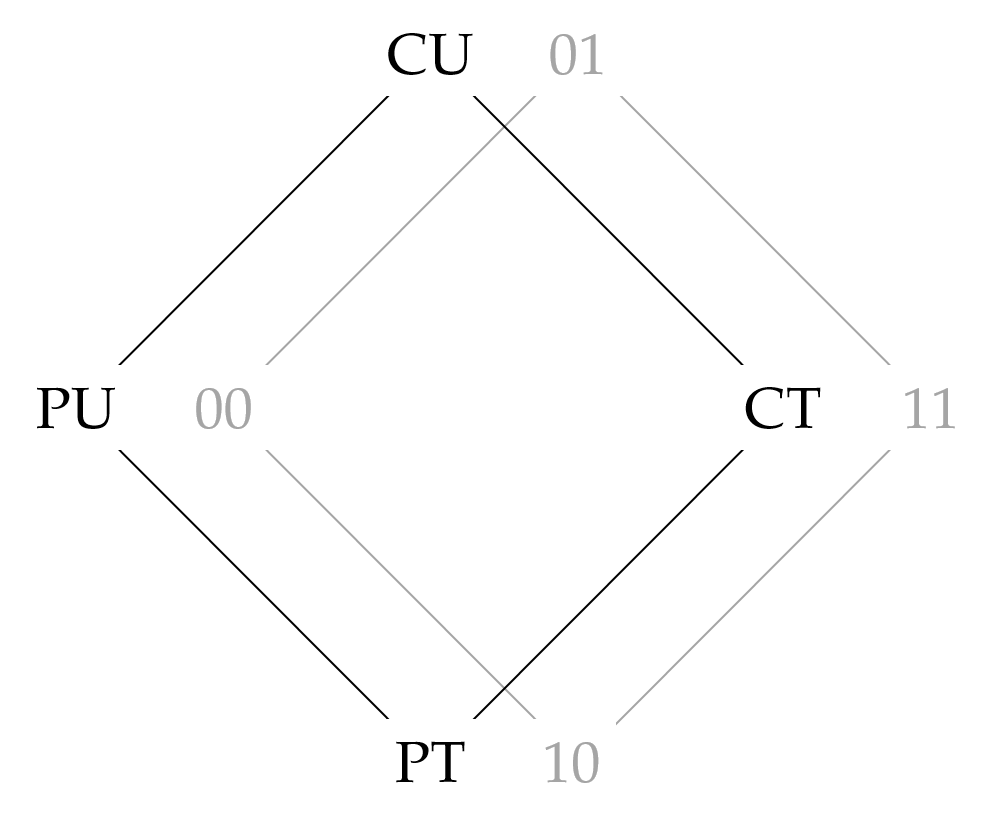
\includegraphics[width=0.4\textwidth]{figures/binary-lattice.png}
    \caption{Security lattice for SecVerilogBL \cite{Ferraiuolo17} with binary equivalent}
    \label{fig:sec-lattice-bin}
\end{figure}

Let $ \sqcup $ be defined on $ \binSigma $ such that $ \varphi $ is an isomorphism, e.g. $ 00 \; \sqcup \; 11 = 10 $.
This mapping is depicted in figure \ref{fig:sec-lattice-bin}.
Note that public and untrusted correspond to a 0 whereas confidential and trusted correspond to a 1.
This abstraction can be formalized by examining two equivalence-relations or -classes on $ \Sigma $ and $ \binSigma $.
We define two partitionings $ \Sigma/_{\equiv_C} $ and $ \Sigma/_{\equiv_I} $ on $ \Sigma $ which induce corresponding equivalence classes of security labels modulo confidentiality $ \equiv_C $ or modulo integrity $ \equiv_I $, respectively.
\begin{align*}
    \Sigma /_{\equiv_C} &= \big\{ \{ \PU, \PT \}, \{ \CU, \CT \} \big\} \\
    \Sigma /_{\equiv_I} &= \big\{ \{ \PU, \CU \}, \{ \PT, \CT \} \big\}
\end{align*}

We coin the names $ \P = [\PU]_{\equiv_C} $, $ \C = [\CU]_{\equiv_C} $, $ \U = [\PU]_{\equiv_I} $ and $ \T = [\PT]_{\equiv_I} $ and lift $ \sqcup $ to be defined on equivalence-classes in the usual fashion, i.e. $ [x] \sqcup [y] = [x \sqcup y] $.
Note that this allows lifting of the $ \preceq $ order on $ \Sigma $ as well, i.e. $ \P \preceq \C $ and $ \T \preceq \U $ where $ \P \preceq \C $ if and only if there is no label $ l_1 \in \C $ such that for any $ l_2 \in \P $ one has $ l_1 \preceq l_2 $, and that all labels can be represented by the intersection of the respective equivalence classes,i.e. $ \{ \PU \} = \P \cap \U $.
Furthermore, it is possible to define $ \sqcup $ solely by working with these equivalence classes:
\begin{equation*}
    \{ x \sqcup y \} = \big(([x]_{\equiv_C} \sqcup [y]_{\equiv_C}) \cap ([x]_{\equiv_I} \sqcup [y]_{\equiv_I}) \big)
\end{equation*}

\begin{example}
    \begin{align*}
        \{ \PU \sqcup \CT \} &= \big(([\PU]_{\equiv_C} \sqcup [\CT]_{\equiv_C}) \cap ([\PU]_{\equiv_I} \sqcup [\CT]_{\equiv_I}) \big) \\
        &= \big((\P \sqcup \C) \cap (\U \sqcup \T) \big) \\
        &= (\C \cap \U) \\
        &= \{ \CU \}
    \end{align*}
\end{example}

This means that labels of the lattice $ (\Sigma, \sqcup, \sqcap) $ can be tracked by considering the confidentiality and integrity parts individually.
In other words: in general one can calculate the supremum or infimum of two labels by performing the respective operation on the parts in the domains of confidentiality and integrity individually.
This is illustrated in figure \ref{fig:lattice-equiv-classes} where again the lattice of security labels is shown but there also are two axes which divide each domain in half.
There, you can see why, e.g. $ \{ \PT \} = \P \cap \T $ and also that $ \P \sqcup \C = \C $ or $ \T \sqcup \U = \U $.

\begin{figure}
    \centering
    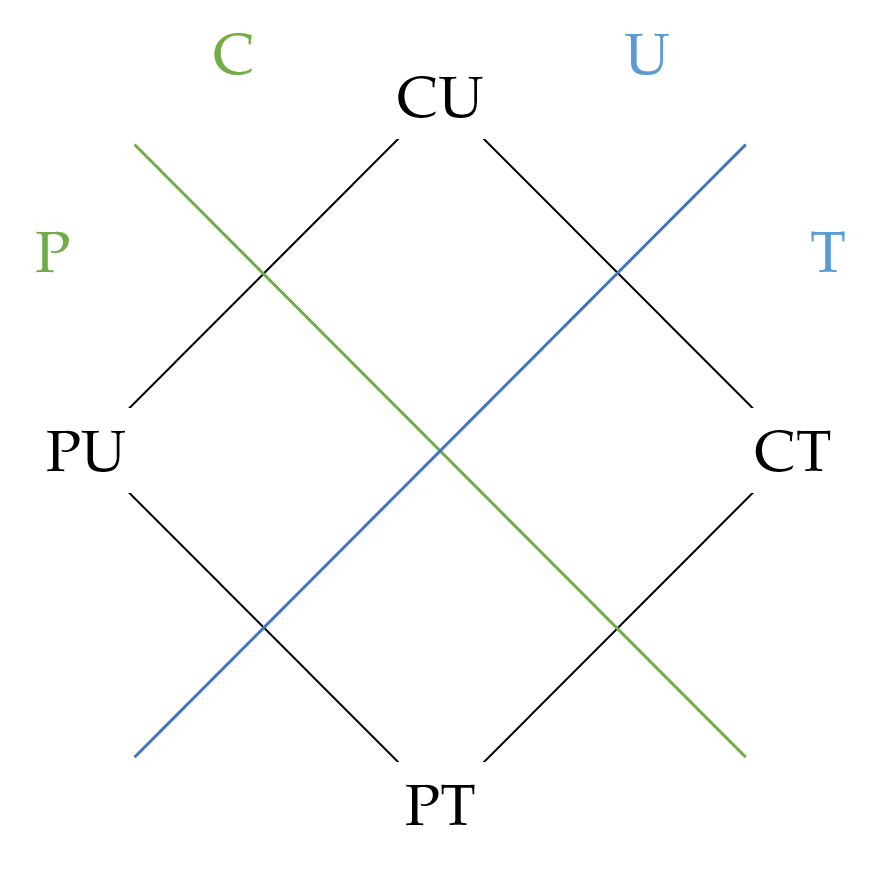
\includegraphics[width=0.4\textwidth]{figures/equivalence-class-lattice.png}
    \caption{Security lattice for SecVerilogBL \cite{Ferraiuolo17} with equivalence-classes}
    \label{fig:lattice-equiv-classes}
\end{figure}

Dealing with information flow labels in this way also is much more intuitive:
\begin{itemize}
    \item Two sources of information combined are considered to be confidential if \textit{any} of the sources is confidential.
    This is sensible as with some result of an operation at least partial knowledge about its confidential source can be inferred- depending on whether the public source or the operation are known.
    \item Two sources of information combined are considered to be trustworthy if \textit{both} of the sources are trustworthy themselves.
    This is intuitive as well.
    Non-trustworthy sources of information are assumed to be controlled by an attacker.
    Some piece of information can only be trustworthy if it can be ensured that the attacker does not control it in any way.
    This is only given if both of the sources of an operation are not controlled by an attacker, i.e. are trustworthy.
\end{itemize}

The intuition behind $ \sqcup $ as described above perfectly matches $ \binSigma $ as well.
Recall, that \C{} is represented by a 1 and \P{} by a 0 in the binary representation.
That means that two labels $ a = a_Ca_I \in \binSigma $ and $ b = b_Cb_I \in \binSigma $ are in \C{}, i.e. confidential, if $ a $ or $ b $ is confidential, i.e. if \textit{one} of the bits representing the confidentiality of the labels is high, i.e. if $ a_C \lor b_C $.
In turn, these two labels are in $ \T $, i.e. trusted, if $ a $ and $ b $ are trusted, i.e. if \textit{both} of the bits representing the integrity of the labels are high, i.e. if $ a_I \land b_I $.
This allows us to define $ \sqcup $ on $ \binSigma $ again - this time not just semantically:
\begin{equation*}
    a_C a_I \sqcup b_C b_I = (a_C \lor b_C) \cdot (a_I \land b_I)
\end{equation*}

In summary, these paragraphs showed to things:
\begin{enumerate}
    \item Information flow labels of information can be tracked by using separate labels for the domain of confidentiality and the domain of integrity which in turn can be stored independently of each other.
    This means that the implementation of the MINRV8 architecture does not need to work with the full lattice of information flow labels itself.
    It is sufficient to deal with equivalence classes which can be inferred from individual bits.
    \item The $ \sqcup $ operation on the binary representation $ \binSigma $ of the security labels can be implemented by concatenating the logical disjunction ($ \lor $) of the confidentiality bits and the logical conjunction ($ \land $) of the integrity bits.
\end{enumerate}

This now allows for adding security label tracking to the model in nuXmv.
Labels are assigned on a per bit basis to all values in registers, memory, \glspl{csr} and the cache.
For each variable in the model, an confidentiality or integrity tracking counterpart as (arrays of) unsigned word(s) is added; find an overview of all such variables in table \ref{tbl:ifc-vars}.

\begin{table}
    \centering
    \begin{tabular}{| c | c | c |}
        \hline
        \textbf{Variable} & \textbf{Confidentiality Tracking} & \textbf{Integrity Tracking} \\
        \hline
        {\smv{regs}} & {\smv{regs_conf}} & {\smv{regs_integrity}} \\
        {\smv{memory}} & {\smv{memory_conf}} & {\smv{memory_integrity}} \\
        {\smv{csrs}} & {\smv{\_\_csrs_conf}} & {\smv{\_\_csrs_integrity}} \\
        {\smv{cache.line}} & {\smv{cache.conf}} & {\smv{cache.integrity}} \\
        \hline
    \end{tabular}
    \caption{Information Flow Tracking Variables}
    \label{tbl:ifc-vars}
\end{table}

These variables transition under the same conditions as their base variable does, e.g. \smv{regs_conf} does a transition if and only if \smv{regs} transitions and \smv{regs_conf} will deduct its content from sources parallel to those of \smv{regs}.
The values themselves change based on the current instruction and its information flow tracking semantics as described in section \ref{sec:ifc-model}.
The only exception to this is the information flow tracking of the variable \smv{csrs} the labels of which do not change at all.
\Glspl{csr} are assigned constants labels because they do not store information but reflect the architectures state.
Certain parts of the architectural state might be for example confidential but the characteristic of being confidential is not determined by the actual value that the respective \gls{csr} is written with but the kind of state that is defined by it.

In other words, the \lstinline[language=SMV,mathescape]{$\dots$_conf} and \lstinline[language=SMV,mathescape]{$\dots$_integrity} variables mirror the architectural part of implementation as described in section \ref{sec:model-implementation}.
The domain of confidentiality and the domain of integrity of the MINRV8 architecture are tracked in addition to simulating the pure computational world where variables implementing the information flow tracking change in parallel to their counterparts in the computational world.

\section{Information Flow Properties}
\label{sec:ifc-properties}

Finally, the information flow properties constituting the information flow control will be defined now.
Each property is expressed as an \gls{ltl} formula of the form \smv{assumptions -> G expr}.
\smv{assumptions} is a macro that will be replaced by a conjunction of assumptions that assume programs running on the architecture to obey the rules to secure usage of the architecture as discussed in \ref{sec:sum-background}.

In the summary of section \ref{sec:ifc-model}, it was mentioned that there are some arguments to the information flow semantic functions in $ \I $ that are not used to determine the information flow label of some architectural word.
These induce the first properties the MINRV8 architecture will be verified against.

Firstly, recall the definition of the LOAD and STORE semantics.
The new tracking labels resulting from executing such an instruction solely depend on the labels of the word loaded or stored.
What has not been used in the definition of information flow is the label of the target address of the memory operation.
It is intuitive that the address does not influence the label of the information itself.
This leads to the following property:
\begin{enumerate}[label=\Roman*.,series=]
    \item \label{itm:prop-mem-i}
    Whenever a memory operation is performed in privileged mode, the target address must be integrous.

    \begin{lstlisting}[
        language=smv,
        caption={Implementation of property \ref{itm:prop-mem-i}},
        label={snpt:prop-mem-i}
    ]
        LTLSPEC NAME MEMORY_OP_INTEGRITY :=
            assumptions -> G (
                priv & op in { LOAD, STORE }
                -> (regs_integrity[rs1] & 0h_03) = 0h_03
            );
    \end{lstlisting}
\end{enumerate}

Secondly, recall the definition of the semantics for \rv{Csrrs} or \rv{Csrrc}, respectively.
These only propagate information flow tracking labels by assigning the constant labels of the \gls{csr} read to the respectively targeted register.
We decided to model the labels of \glspl{csr} as constants because they control the state of the architecture and as such might be target of an attack.
We labelled all \glspl{csr} as integrous and \gls{mstatus} as confidential.
We decided to not label \gls{pmacfg} or \gls{pmpcfg} as confidential since it can be assumed that user mode must be able to know where memory regions are to operate correctly.

Coming back to the information flow semantics of \rv{Csrrs} and \rv{Csrrc}, notice that in the respective definition of the semantical functions the value, the \glspl{csr} are written with, is not used.
This must necessarily be the case since the labels of the \glspl{csr} are constant and as such cannot change based on the labels of the value to write them with.
However, this leads us to phrase a property about the \gls{csr} labels that ensures their integrity:
\begin{enumerate}[label=\Roman*.,resume]
    \item \label{itm:prop-csr-i}
    Whenever a \gls{csr} is written, the value it is written with must be integrous.

    \begin{lstlisting}[
        language=smv,
        caption={Implementation of property \ref{itm:prop-csr-i}}
    ]
        LTLSPEC NAME CSR_INTEGRITY :=
            assumptions -> G (
                priv & op in { CSRRS, CSRRC }
                -> regs_integrity[rs2] = 0h_FF
            );
    \end{lstlisting}
\end{enumerate}

Both of these properties are founded in intuition as well.
It is not safe to have an attacker control the load and store instructions of machine-mode since this could lead to unwanted behavior of code.
One might object that this is not problematic since, if a malicious value was to be loaded by machine-mode, information flow tracking should catch this, however, this must not necessarily be the case.
An attacker could trick machine-mode into using a value that is labelled as integrous but coincidentally diverges the control flow of machine-mode in a way that is beneficial to an attacker.
Additionally, it is obvious that \glspl{csr} should only be written with trusted data.

From all the variables our implementation of the MINRV8 architecture comprises we now considered \smv{regs} and \smv{memory} as well as \smv{cache} in regards to the security of the architecture by looking at the gaps of the information flow semantic functions.
We also considered the variable \smv{csrs} by assigning constant information flow labels to it and using it as an information flow target, i.e. we phrased properties ensuring that certain flows of information \textit{to} \smv{csrs} do not occur.
However, up to this point the \smv{priv} variable which holds the current privilege mode was only handled implicitly.
It was used as a source of labels since it determines the labels of machine words loaded as immediates by LOADI.

It is reasonable to assume, though, that \smv{priv} also can serve as an information flow target - similar to \smv{csrs}.
We already did this partially for property \ref{itm:prop-mem-i} where we assumed the architecture to be in privileged mode.
These properties, however, only dealt with the integrity labels of information.
The domain of confidentiality has yet been left out so we will introduce one final property for verification that covers the interplay between privilege mode and confidentiality labels:
\begin{enumerate}[label=\Roman*.,resume]
    \item \label{itm:prop-no-leak}
    Whenever the architecture is in user mode, there is no confidential data in any register.

    \begin{lstlisting}[
        language=smv,
        caption={Implementation of property \ref{itm:prop-no-leak}},
        label={snpt:prop-no-leak}
    ]
        LTLSPEC NAME NO_LEAK :=
            assumptions -> G (priv | (
                regs_conf[0] = 0h_00
                & regs_conf[1] = 0h_00
                & regs_conf[2] = 0h_00
                & regs_conf[3] = 0h_00
            ));
    \end{lstlisting}
\end{enumerate}

\section{Summary}

In this chapter, information flow semantics were given for each instruction of the MINRV8 architecture and it was described how these were implemented in nuXmv.
It was shown that the domains of confidentiality and integrity of the information flow policy can be tacked independently where the $ \sqcup $ operation on confidentiality labels is given by the logical disjunction and on integrity labels by the logical conjunction.

Labels of arguments to some instructions that are not used by their respective information flow semantics were used to constitute the first information flow properties regarding integrity of instructions.
Additionally, the \smv{priv} variable was considered when defining a property touching the confidentiality of data.
In the end, all variables of the main module and all labels of arguments to instructions were considered such that they either led to an information flow property or are used to determine information flow in the model.

The properties that were finally established are:
\begin{enumerate}[label=\Roman*.]
    \item \smv{MEMORY_OP_INTEGRITY}: whenever a memory operation is performed in privileged mode, the target address must be integrous.
    \item \smv{CSR_INTEGRTY}: whenever a \gls{csr} is written, the value it is written with must be integrous.
    \item \smv{NO_LEAK}: whenever the architecture is in user mode, there is no confidential data in any register.
\end{enumerate}

\begin{figure}
    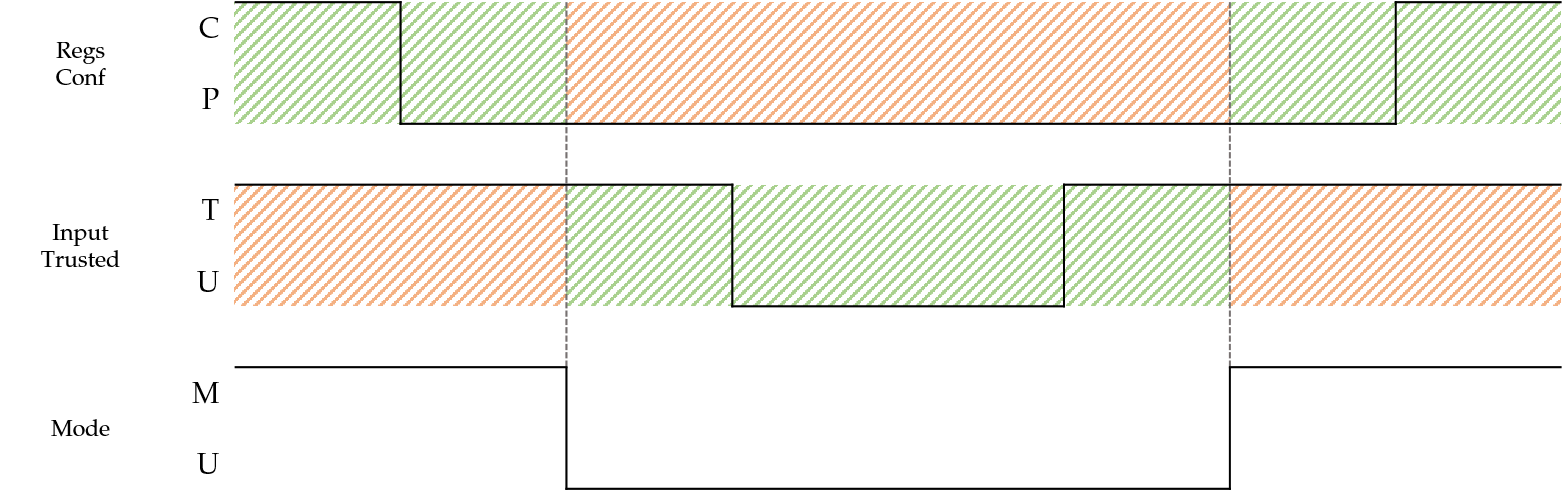
\includegraphics[width=\textwidth]{figures/properties.png}
    \caption{Visualization of the Information Flow Properties}
    \label{fig:ifc-properties}
\end{figure}

These properties are visualized in figure \ref{fig:ifc-properties} inspired by digital timing diagrams.
The last row visualizes the privilege mode of the architecture over the course of executing a sequence of instructions.
There are two points in which the privilege mode changes: first, it changes from machine- to user-mode, then it changes back from user- to machine-mode.
The \smv{NO_LEAK} property (\ref{itm:prop-no-leak}) mandates that the confidentiality labels of the registers always resemble the first row in the diagram, i.e. they are only high when the current privilege mode also is high.
The green areas highlight where the registers could contain confidential data, i.e. the confidentiality  labels \textit{could} be high, but the orange areas highlight the point in time where the confidentiality labels \textit{must} be low.
The properties \smv{MEMORY_OP_INTEGRITY} (\ref{itm:prop-mem-i}) and \smv{CSR_INTEGRITY} (\ref{itm:prop-csr-i}) follow the same visualization.
In the second row of the figure, it is visualized whether inputs to memory or \gls{csr} related instructions are integrous.
The integrity labels to input of these instructions must be high, whenever the architecture is in machine-mode and can be low if the architecture is on user-mode.
Analogously, the green areas mark where the integrity labels \textit{could} be low but the orange areas indicate where it \textit{must} be high.

\section{Checking}
\label{sec:checking}

In this section we will outline the process of the actual \textit{verification} of the now implemented architecture.
The verification process itself is threefold:
Before any verification can be done, it needs to be clear what shall be verified - not in the sense what the object of verification is but what its goal is, i.e. which properties express the security of the architecture adequately?
This allows the actual verification of these properties as the next step which will lead to first results.
In the case of a real world verification attempt these results hopefully are that the system to be verified is perfectly valid - it is, however, most likely that the majority of properties verified will end up with a negative result.
In this case, the model and/or properties are refined which marks the last step.

Not only will we detail these steps themselves, we will also reflect whether this process of verification is trustworthy by shedding light on the methodology of deriving the concretization of these by now only loosely described steps.
To outline this, we will answer two questions:
How do we phrase properties to verify?
How do we refine the model and/or properties on a verification failure?

\subsection{Verification Process}

\subsubsection{Properties}

In the summary of section \ref{sec:ifc-model} we mentioned that there are some arguments to the information flow semantic functions in $ \I $ that are not used to determine the information flow label of some architectural word.
These induce the first properties we will verify the MINRV8 architecture against.

Firstly, recall the definition of the LOAD and STORE semantics.
The new tracking labels resulting from executing such an instruction solely depend on the labels of the word loaded or stored.
What hasn't been used in the definition of information flow is the label of the target address of the memory operation.
It is intuitive that the address does not influence the label of the information itself.
% TODO: is security a good word?
However, this suggests that the labels of the address of the memory operation might be relevant for the security of architecture as a whole in another.
This leads to the following two properties:
\begin{enumerate}[label=\Roman*.,series=]
    \item \label{itm:prop-mem-i}
    Whenever a memory operation is performed in privileged mode, the target address must be integrous.
    \item \label{itm:prop-mem-c}
    Whenever a confidential word is read from or written to memory in privileged mode, the target address must be confidential.
\end{enumerate}

% TODO: give intuition for both properties

Secondly, recall the definition of the semantics for CSRRS or CSRRC, respectively.
These only propagate information flow tracking labels by assigning the constant labels of the \gls{csr} read to the respectively targeted register.
We decided to model the labels of \glspl{csr} as constants because they control the state of the architecture and as such might be target of an attack.
We labelled all \glspl{csr} as integrous and \gls{mstatus} as confidential.
We decided to not label \gls{pmacfg} or \gls{pmpcfg} as confidential since it can be assumed that user mode must be able to know where memory regions are to operate correctly.
Our architecture does not support virtual addresses, address translation or other similar concepts which might hide details of the memory settings from user mode leaving it without the need to know the details of memory settings.

Coming back to the information flow semantics of CSRRS and CSRRC, notice that in the respective definition of the semantical functions the value the \glspl{csr} are written with is not used.
This must necessarily be the case since the labels of the \glspl{csr} are constant and as such can not change based on the labels of the value to write them with.
However, this leads us to phrase a property about the \gls{csr} labels that ensures their integrity or confidentiality respectively:
\begin{enumerate}[label=\Roman*.,resume]
    \item \label{itm:prop-csr-i}
    Whenever a \gls{csr} is written, the value it is written with must be integrous.
    \item \label{itm:prop-mstatus-c}
    Whenever \gls{mstatus} is written, the value it is written with must be confidential.
\end{enumerate}

From all the variables our implementation of the MINRV8 architecture comprises we now considered \smvinline{regs} and \smvinline{memory} as well as \smvinline{cache} in regards to the security of the architecture by looking at the gaps of the information flow semantic functions.
We also considered the variable \smvinline{csrs} by assigning constant information flow labels to it and using it as an information flow target, i.e. we phrased properties ensuring that certain flows of information \textit{to} \smvinline{csrs} do not occur.
However, up to this point we only implicitly handled the \smvinline{priv} variable which holds the current privilege mode.
It was used as a source of labels since it determines the labels of machine words loaded as immediates by LOADI.

It is reasonable to assume, though, that \smvinline{priv} also can serve as an information flow target; similar to \smvinline{csrs}.
We already did this partially in properties \ref{itm:prop-mem-i}and \ref{itm:prop-mem-c} where we assumed the architecture to be in privileged mode.
These properties, however, only dealt with the integrity labels of information.
The domain of confidentiality has yet been left out so we will introduce one final property for verification that covers the interplay between privilege mode and confidentiality labels:
\begin{enumerate}[label=\Roman*.,resume]
    \item \label{itm:prop-no-leak}
    Whenever the architecture is in user mode, there is no confidential data in any register.
\end{enumerate}

The implementation of these five properties is straight-forward.
Confer code snippets \ref{snpt:prop-mem-i}-\ref{snpt:prop-no-leak} for details.

\begin{smv}[caption={Implementation of property \ref{itm:prop-mem-i}},label={snpt:prop-mem-i}]
INVARSPEC NAME MEMORY_OP_INTEGRITY :=
    (priv & op in { LOAD, STORE })
    -> regs_integrity[rs1] > 0h_03;
\end{smv}

\begin{smv}[caption={Implementation of property \ref{itm:prop-mem-c}}]
INVARSPEC NAME MEMORY_OP_CONFIDENTIALITY :=
    (priv & op in { LOAD, STORE }
        & memory_conf[read_addr(rs1)] > 0h_00)
    -> regs_conf[rs1] > 0h_03;
\end{smv}

\begin{smv}[caption={Implementation of property \ref{itm:prop-csr-i}}]
INVARSPEC NAME CSR_INTEGRITY :=
    (priv & op in { CSRRS, CSRRC })
    -> regs_integrity[rs2] = 0h_FF;
\end{smv}

\begin{smv}[caption={Implementation of property \ref{itm:prop-mstatus-c}}]
INVARSPEC NAME MSTATUS_CONFIDENTIALITY :=
    (priv & op in { CSRRS, CSRRC })
    -> regs_conf[rs2] > 0h_0F;
\end{smv}

\begin{smv}[caption={Implementation of property \ref{itm:prop-no-leak}},label={snpt:prop-no-leak}]
INVARSPEC NAME NO_LEAK := priv | (
    regs_conf[0] = 0h_00
    & regs_conf[1] = 0h_00
    & regs_conf[2] = 0h_00
    & regs_conf[3] = 0h_00
);
\end{smv}

\subsubsection{Mitigations \& Refinement}

\subsection{Trustworthiness of the Verification Process}

%!TEX root = ../thesis.tex

\chapter{Results}
\label{chp:results}

This section will cover the results of the verification process as it was described in section \ref{sec:sum-background}.
Our main finding is that there are 8 assumptions which in total grant that the properties as described in section \ref{sec:ifc-properties} can not be violated, in other words: the MINRV8 architecture models the information flow properties introduced in this thesis, namely \smv{MEMORY_OP_INTEGRITY}, \smv{CSR_INTEGRITY} and \smv{NO_LEAK}, if and only if the 8 assumptions that will be introduced in subsequent sections are in place.

Additionally, roughly 23 bug fix patches\footnote{%
    The number of 23 bug fix patches was measured by counting the amount of patches containing the word \enquote{fix} in its description and being applied to the model file.
} were applied to the model and some \smv{INIT} constraints were set up.
Taken together with aforementioned assumptions these patches mark a fixpoint of the prove-refine loop discussed in section \ref{sec:sum-background} and depicted in figure \ref{fig:ver-process}.

This section is grouped as follows: section \ref{sec:assumptions} will introduce aforementioned assumptions and \smv{INIT} constraints.

Note that only assumptions and no architectural refinements were introduced to the model\footnote{%
    It was tested whether two assumptions could be replaced by one architectural mitigation.
    It turned out, however, that this architectural refinement did not manage to rule out the respective vulnerability.
    This is discussed at the end of appendix \ref{app:cexs}.
}.
It therefore was also tested how the results would change when canaries are introduced to the architecture.
The term \enquote{canary} refers to the birds used in coal mines to indicate a loss of oxygen.
In the field of software development, this term refers to bugs that are added to code bases deliberately in order to test detection mechanisms.
These canaries mimic known vulnerabilities to real-world architectures and will therefore also give an overview of the capabilities of the verification approach of this thesis.
The results of these tests will finally be presented in section \ref{sec:canaries}.

\section{Assumptions}

Technically, \smv{INIT} constraints and assumptions serve the same purpose: They limit the state spaces that will be searched for property violations.
Conceptually, however, these two concepts should be distinguished.
In the model, \smv{INIT} constraints are used to limit the search of the state space to \textit{valid} counter-examples only.
Validity here means, that properties are not false to begin with and that the initial state of the architecture complies with the specification.
Consequently, these constraints were introduced during the prove-refine loop as fixes to the model.
Assumptions on the other hand are not part of the model in a technical sense but mark a result of the verification of the architecture: Each assumptions constitutes a rule for e.g. \gls{os} or compiler engineers to obey in order to write or generate non-vulnerable code.

\subsection{Initial Constraints}

Validity of the counter-examples was guaranteed by 13 \smv{INIT} constraints that can be grouped into four categories.
Firstly, two groups of constraint guarantee that counter-examples are not false upfront.
By constraining the contents of registers to only contain confidential data when the architecture starts in machine-mode and to only contain malicious data when the architecture starts in user-mode.
Furthermore, cache and memory can only contain confidential data if the respective memory region is set to \textit{not} be readable for user-mode and can only contain malicious data if the respective memory region \textit{is} set to be writable by user-mode.
If, for example, the model would not be constrained to initially only contain confidential data in some register when in machine-mode, nuXmv returns a trivial counter-example violating the \smv{NO_LEAK} property (\ref{itm:prop-no-leak}) where the architecture starts in user-mode and has confidential data in some register.

Secondly, two more group of constraints ensures the initial state to comply with the specification is guaranteed.
The first is rather simple, given by a single constraint and depicted in the following snippet:
\begin{lstlisting}[
    language=smv,
    caption={\gls{mstatus} \smv{INIT} constraint for the model}
]
    INIT MIE = 0b_1 -> MPP = 0b_0;
\end{lstlisting}
This constraint ensures that the interrupt handling mechanisms are set up correctly as mandated by the RISC-V specification (cf. section \ref{sec:rv-priv-arch} and figure \ref{fig:interrupt-handling}).
As \smv{MPP} is cleared on return from a trap handler and \smv{MIE} being high implies that no interrupt is being handled at the moment, \smv{MPP} must be low.

The last group of constraints sets up caching errorless, i.e. if the cache is valid, it can only point to an address of a region that is cacheable and must match that addresses content unless the respective region is set to be write-back-cacheable.

\subsection{Property Assumptions}
\label{sec:assumptions}

\begin{table}
    \centering
    \begin{tabular}{| c r | c | c | c |}
        \multicolumn{1}{r}{} & \multicolumn{1}{r}{} &
        \multicolumn{1}{l}{\tilthdr{\smv{MEMORY_OP_INTEGRITY} (\ref{itm:prop-mem-i})}} &
        \multicolumn{1}{l}{\tilthdr{\smv{CSR_INTEGRITY} (\ref{itm:prop-csr-i})}} &
        \multicolumn{1}{l}{\tilthdr{\smv{NO_LEAK} (\ref{itm:prop-no-leak})}} \\
        \hline % \cline{3-5}
        \multirow{2}{*}{Mode-boundary} & \smv{SAN_ON_CALL} & \checkmark & \checkmark & \\
        \cline{3-5}
        & \smv{CLR_ON_RET} &&& \checkmark \\
        \hline % \cline{3-5}
        \multirow{2}{*}{Memory} & \smv{NO_PUBLIC_READS} & \checkmark & \checkmark & \\
        \cline{3-5}
        & \smv{NO_PUBLIC_WRITES} &&& \checkmark \\
        \hline % \cline{3-5}
        \multirow{4}{*}{Memory privilege} & \smv{SAN_ON_CLASSIFICATION} & \checkmark & \checkmark & \\
        \cline{3-5}
        & \smv{CLR_ON_DECLASSIFICATION} &&& \checkmark \\
        \cline{3-5}
        & \smv{SAN_CACHE_ON_CLASSIFICATION} & \checkmark & \checkmark & \\
        \cline{3-5}
        & \smv{CLR_CACHE_ON_DECLASSIFICATION} &&& \checkmark \\
        \hline % \cline{3-5}
    \end{tabular}
    \caption{Assumptions Compared to Properties}
    \label{tbl:assumptions-overview}
\end{table}

During the prove-refine loop, whenever it was found that a counter-example to a property reported by nuXmv was valid and not an actual vulnerability of the architecture but a risk to be controlled by software, an assumption was phrased resembling a mitigation of the respective vulnerability.
This led to a total number of eight assumptions which in total grant the absence of any information flow control violation.
These assumptions can be grouped into three categories:
\begin{itemize}
    \item Mode-boundary crossing related assumptions
    \item Memory related assumptions
    \item Memory privilege related assumptions
\end{itemize}

Find an overview of all these assumptions in table \ref{tbl:assumptions-overview}.
Each row represents one assumption and each column one property.
A check mark denotes that the respective assumption is critical for the respective property, i.e. there exists a counter-example proving the property to be false if the assumption at hand is not assumed.
These counter-examples are given in detail in appendix \ref{app:cexs} and will be skipped here.

Note that each of the assumptions is critical for at least one property.
This shows that \enquote{$ \text{assumptions} \Leftrightarrow \text{properties} $} as opposed to only \enquote{$ \text{assumptions} \Rightarrow \text{properties} $} since \enquote{$ \neg \text{assumptions} \Rightarrow \neg \text{properties} $}.

\paragraph{Mode-boundary crossing related assumptions}
As can be seen in table \ref{tbl:assumptions-overview}, there are two properties related to mode-boundary crossing.
Mode-boundary crossing related here refers to vulnerabilities that violate a property at execution of the \smv{Ecall} or \smv{Mret} instruction.

The first of these is called \smv{SAN_ON_CALL} and mandates from machine-mode to not use \textit{dangerous} instructions before having cleared the registers from any untrusted data when entering machine- from user-mode.
Dangerous instructions here are \minrv{Load}, \minrv{Store}, \minrv{Csrrs} and \minrv{Csrrc} and directly stem from the instructions used in properties \smv{MEMORY_OP_INTEGRITY} (\ref{itm:prop-mem-i}) and \smv{CSR_INTEGRITY} (\ref{itm:prop-csr-i}).
The next assumption to be introduced is called \smv{CLR_ON_RET}; it states: Whenever machine-mode hands back control to user-mode, the registers must be cleared of any confidential information.
The implementation of \smv{SAN_ON_CALL} and \smv{CLR_ON_RET} can be found in snippet \ref{snpt:san-on-call} and \ref{snpt:clr-on-ret} respectively.

Taken together, these two assumptions ensure that machine-mode neither directly hands secrets to nor directly is handed malicious data by user-mode.

\begin{figure}
    \begin{lstlisting}[
        language=smv,
        caption={Assumption \lstinline{SAN_ON_CALL}},
        label={snpt:san-on-call}
    ]
        G (!priv & X priv -> X (
            (priv -> !(op in { LOAD, STORE, CSRRS, CSRRC }))
            U (regs_integrity[0] = 0h_FF
                & regs_integrity[1] = 0h_FF
                & regs_integrity[2] = 0h_FF
                & regs_integrity[3] = 0h_FF)
        ))
    \end{lstlisting}

    \begin{lstlisting}[
        language=smv,
        caption={Assumption \smv{CLR_ON_RET}},
        label={snpt:clr-on-ret}
    ]
        G (
            priv & X !priv -> regs_conf[0] = 0h_00
                & regs_conf[1] = 0h_00
                & regs_conf[2] = 0h_00
                & regs_conf[3] = 0h_00
        )
    \end{lstlisting}
\end{figure}

Both assumptions \smv{SAN_ON_CALL} and \smv{CLR_ON_RET} are similar to each other.
Both were introduced under the label of being \textit{mode-boundary crossing related}, which means that both assumptions are about information flow tracking labels when changing privilege mode - more precisely: both are about the labels of register contents.
The relation of these two assumptions, however, also characterizes a pattern that can also be recognized for subsequent groups of assumptions.
It turned out that for every integrity related assumption, such as \smv{SAN_ON_CALL}, there was a similar confidentiality related assumption such as \smv{CLR_ON_RET}.
This can be easily seen in table \ref{tbl:assumptions-overview}.
In alternating rows, two groups of assumptions can be distinguished: those which are relevant to the properties \smv{MEMORY_OP_INTEGRITY} and \smv{CSR_INTEGRITY} and those which are relevant to the property \smv{NO_LEAK}.
Additionally it is noteworthy that these two groups of assumptions can be characterized by the way they constrain information flow.
Whereas confidentiality related assumptions always constrain flow of information going \textit{out of} machine-mode, integrity related assumptions always constrain flow of information going \textit{into} machine-mode.

\paragraph{Memory related assumptions}
Two assumptions about memory reads and writes join the ranks of these groups, namely \smv{NO_PUBLIC_READS} and \smv{NO_PUBLIC_WRITES} which are formally given in snippet \ref{snpt:no-public-reads} and \ref{snpt:no-public-writes} respectively.
These two assumptions don't express more than the title says; they require machine-mode to never read from or write to public memory.
As such, they directly extend the mode-boundary related assumptions.
At first, it was ensured that machine-mode neither hands out secrets nor accepts malicious data directly.
These two assumptions now ensure that the same must not happen by a detour into memory.

\begin{figure}
    \begin{lstlisting}[
        language=smv,
        caption={Assumption \lstinline{NO_PUBLIC_READS}},
        label={snpt:no-public-reads}
    ]
        G (priv & op = LOAD -> (
            mem_addr < $REGION0_SIZE
                ? !pmpcfg0.write
                : !pmpcfg1.write
        ))
    \end{lstlisting}

    \begin{lstlisting}[
        language=smv,
        caption={Assumption \lstinline{NO_PUBLIC_WRITES}},
        label={snpt:no-public-writes}
    ]
        G (priv & op = STORE -> (
            mem_addr < $REGION0_SIZE
                ? !pmpcfg0.read
                : !pmpcfg1.read
        ))
    \end{lstlisting}
\end{figure}

\paragraph{Memory privilege related assumptions}
The four assumptions that have been introduced up to this point seem to cover all relevant channels of information transmission: registers and memory.
However, these are not enough to ensure that the MINRV8 architecture implements all information flow properties subject to this thesis.
Whereas the two memory related properties covered the group of actions by machine-mode where information directly is given to or taken from user-mode, it is also possible to transmit information indirectly via memory by writing it to or reading it from safe memory regions but then changing the attributes of respective memory regions.
The two assumptions \smv{SANITIZE_ON_DECLASSIFICATION} and \smv{CLR_ON_DECLASSIFICATION} counter issues arising from these vectors.
The former assumption demands from machine-mode to ensure that a memory region does not contain malicious information when its set to be publicly inaccessible.
This assumption is formalized in snippet \ref{snpt:san-on-classify}.
The latter demands from machine-mode to always ensure that a memory region does not contain confidential information when its made publicly accessible.
This assumption is formalized in snippet \ref{snpt:clr-on-declassify}.

\begin{figure}
    \begin{lstlisting}[
        language=smv,
        caption={Assumption \lstinline{SAN_ON_CLASSIFICATION}},
        label={snpt:san-on-classify}
    ]
        G (pmpcfg0.write & X !pmpcfg0.write
            -> memory_integrity[0] = 0h_FF
             & memory_integrity[1] = 0h_FF)
        & G (pmpcfg1.write & X !pmpcfg1.write
            -> memory_integrity[2] = 0h_FF
             & memory_integrity[3] = 0h_FF)
    \end{lstlisting}

    \begin{lstlisting}[
        language=smv,
        caption={Assumption \lstinline{CLR_ON_DECLASSIFICATION}},
        label={snpt:clr-on-declassify}
    ]
        G (!pmpcfg0.read & X pmpcfg0.read
            -> memory_conf[0] = 0h_00
             & memory_conf[1] = 0h_00)
        & G (!pmpcfg1.read & X pmpcfg1.read
            -> memory_conf[2] = 0h_00
             & memory_conf[3] = 0h_00)
    \end{lstlisting}
\end{figure}

Yet, these two assumptions still not suffice to grant the absence of memory privilege related property counter-examples.
It turns out that only ensuring memory regions to not contain confidential/malicious words when (de-)classifying respective regions allows problematic data to remain in cache which bypasses \smv{SAN_ON_CLASSIFICATION} and \smv{CLR_ON_DECLASSIFICATION}.
This brings the need to also assume that the cache is cleared and sanitized by the architecture whenever a memory region is (de-)classified.
This is expressed in the assumptions \smv{SAN_CACHE_ON_CLASSIFICATION} and \smv{CLR_CACHE_ON_DECLASSFICATION} (cf. snippets \ref{snpt:sanc-on-classify}, \ref{snpt:clrc-on-declassify}).

To summarize all assumptions:
At first, \smv{SAN_ON_CALL} and \smv{CLR_ON_RET} assumed that no direct flow of sensitive or malicious data is possible between user- and machine-mode (snippets \ref{snpt:san-on-call} and \ref{snpt:clr-on-ret}).
Then, these assumptions were generalized to rule out detours into memory by \smv{NO_PUBLIC_WRITES} and \smv{NO_PUBLIC_READS} (snippets \ref{snpt:no-public-writes} and \ref{snpt:no-public-reads}).
Finally, it was assumed that machine-mode must not freely alter access privileges of memory regions.
It must clear or sanitize regions accordingly, depending on the previous access privileges, e.g. machine-mode must ensure to not forget secrets in memory that is made publicly accessible.

\begin{figure}
    \begin{lstlisting}[
        language=smv,
        caption={Assumption \lstinline{SAN_CACHE_ON_CLASSIFICATION}},
        label={snpt:sanc-on-classify}
    ]
        G (pmpcfg0.write & X !pmpcfg0.write
                & cache.valid & cache.addr < $REGION0_SIZE
            -> cache.integrity = 0h_FF) &
        G (pmpcfg1.write & X !pmpcfg1.write
                & cache.valid & $REGION0_SIZE <= cache.addr
            -> cache.integrity = 0h_FF)
    \end{lstlisting}

    \begin{lstlisting}[
        language=smv,
        caption={Assumption \lstinline{CLR_CACHE_ON_DECLASSIFICATION}},
        label={snpt:clrc-on-declassify}
    ]
        G (!pmpcfg0.read & X pmpcfg0.read
                & cache.valid & cache.addr < $REGION0_SIZE
            -> cache.conf = 0h_00) &
        G (!pmpcfg1.read & X pmpcfg1.read
                & cache.valid & $REGION0_SIZE <= cache.addr
            -> cache.conf = 0h_00)
    \end{lstlisting}
\end{figure}

\section{Canaries}
\label{sec:canaries}

In this section, it will be presented how the model of the MINRV8 architecture was altered in order to implement real-world attacks to the Intel x86 architecture.
By default, the MINRV8 architecture is not vulnerable to these attacks, however, making the architecture vulnerable will put the approach of this thesis to formally verify an instruction set architecture to a test.

\subsection{Cache Poisoning Attack on x86}

The cache poisoning attack\footnote{%
    The name \enquote{cache poisoning attack} is not official.
} was discovered and presented by Rafal Wojtczuk and Joanna Rutkowska in their publication \textit{Attacking SMM Memory via Intel CPU Cache Poisoning} \cite{Wojtczuk09}.
\enquote{SMM memory} refers to a specific region of memory that is designed to be only accessible by the mode of highest privilege in x86 architectures: System Management Mode.
This memory is intended to be written only on start-up and then locked down for later write-accesses.
Wojtczuk and Rutkowska, however, managed to find a vulnerability to the x86 architecture which allowed them to effectively write to SMM memory without SMM privileges by marking respective memory region as write-back-cacheable.
The attack comprises the following steps and requires administrator privileges on the machine to be attacked:
\begin{enumerate}
    \item Mark SMM memory as write-back-cacheable using administrator privileges
    \item \label{itm:cache-pois-mem}
    Generate write accesses to the memory.
    Since the region is marked as write-back-cacheable, the writes will not be propagated to the memory controller which would drop these accesses but will be cached.
    \item \label{itm:cache-pois-smi}
    Trigger an System Management Interrupt to transfer control to System Management Mode.
    Depending on the specific addresses written System Management Mode will now execute code written with administrator privileges in step \ref{itm:cache-pois-mem}.
\end{enumerate}

Steps \ref{itm:cache-pois-mem} and \ref{itm:cache-pois-smi} can also be swapped to read from SMM memory.
Then, triggering the interrupt will make SMM mode execute parts of SMM memory which will leave some parts of the handler being cached.
After SMM returns from handling the interrupt, administrator mode can read these words from cache.

This attack does not fully apply to the MINRV8 architecture since it does not support as fine grained privilege modes as the x86 architecture.
In x86, administrator privileges are needed to set SMM memory cacheable and attack SMM-mode which is of higher privilege than administrator-mode.
To apply this attack to the MINRV8 would bring the need of user-mode being able to set cacheability properties of memory regions.
It is not reasonable to assume that anyone would give user-mode this power.
However, the basic idea can still be implemented by following changes to the model:
\begin{itemize}
    \item For all cache transition relations, do not check whether current privilege mode suffices for the memory operation at hand, i.e. user-mode can write to cache of memory regions not set as writable to it.
    \item For load accesses to memory, do not check whether current privilege mode suffices for the memory read if the address is being cached, i.e. user-mode can read cached memory regions even if they're not set as readable to it.
\end{itemize}

These changes manage to introduce a vulnerability to the MINRV8 architecture.
If assuming all assumptions introduced in section \ref{sec:assumptions}, nuXmv manages to find a counter-example for all three information flow properties.
These, again, are discussed in the appendix (cf. \ref{sec:cexs-cache-vuln}).

\todo[inline]{Fix text flow}

One distinction from the original cache-poisoning attack to these counter-examples is that here, the attacker can't set the attacked memory region to be cacheable in the first place.
This difference does not play a major role since the attack can take place nonetheless if some memory region happens to be locked down to user-mode and is set to be write-back-cacheable, still this weakens the attack to some degree.

What can be done to mitigate this attack?
Obviously, the vulnerability purposefully introduced to the architecture could be dropped.
At this point, though, it is not clear how realistic this characteristic of the MINRV8 architecture is since at least in the case of the x86 architecture, the findings of \cite{Wojtczuk09} suggest hardware does not perform privilege checks when writing to the cache.

It not likely, however, that RISC-V is vulnerable to this attack.
One the one hand, the specification states that cacheability settings can be modified by machine-mode only \cite[p.43]{RiscVISAP}.
One the other hand, it also states that \gls{pmp} attributes (including access privileges) are checked in \textit{parallel} to \glspl{pma} (defining cacheability), i.e. regardless of cacheability settings, and always trap at privilege violations \cite[44-45]{RiscVISAP}.
This indicates that neither would a privilege mode other than machine-mode be able to set any memory region cacheable nor would it be able to read from cache of memory regions it otherwise does not have access to.
It should be part of future work, though, to implement a complete model of the RISC-V specification which would verify whether RISC-V is actually not susceptible to this attack vector.

\subsection{The SYSRET Vulnerability}
\label{sec:sysret}

The so called \textit{SYSRET vulnerability} to the intel x86 architecture is listed as vulnerability \textit{CVE-2012-0217} by the \textit{Common Vulnerabilities and Exposures} database (CVE\textsuperscript{\textregistered}) \cite{SYSRET-vuln} and allegedly has also been found by Rafal Wojtczuk \cite{SYSRETFreeBSD,SYSRETDebian,SYSRETCert}.
To our knowledge, the most concise and freely available explanation of the vulnerability can be found in the blog post \textit{The Intel SYSRET Privilege Escalation} by George Dunlap published on the page of Xen Project, a community for virtualization-related open source projects which in part also have been affected by said vulnerability \cite{Dunlap19}.

The x86 architecture provides multiple ways to switch between privilege modes.
In principle, these ways work analogously to how the MINRV8 architecture changes privilege modes: either an interrupt/exception leads to the privilege escalation or a dedicated instruction is executed that changes privilege mode, e.g. \minrv{Ecall} in case of the MINRV8 architecture.
In general, when changing the privilege mode, the \lstinline{RIP} register, which is the \gls{pc} equivalent for x86 architectures, and the stack-pointer are set to the respective version of the targeted privilege-mode.
The designers of the architecture, however, found that parts of the normal privilege mode changing routines could be left out in some scenarios to improve performance.
One of this routines to be left out was changing the stack-pointer by hardware.
These performance improvements are implemented in the \lstinline{SYSCALL} instruction which makes a cheap transition to high-privilege mode by for instance not changing the stack-pointer by hardware.
In consequence, there is the analogous \lstinline{SYSRET} instruction to return control back to user-mode which also does not set the stack-pointer.
However, if an interrupt handler invoked by the \lstinline{SYSCALL} instruction intends to use the stack-pointer, it must first set the stack-pointer up accordingly and afterwards set it back to user-mode\footnote{%
    There are more than two privilege modes provided by the x86 architecture and they also have different names than the privilege modes of the MINRV8 architecture, however, the SYSRET vulnerability only touches two privilege modes with have the same purpose as user- and machine-mode in the case of the MINRV8 architecture.
    Therefore, in this context, the terms user-mode and machine-mode will also be used to talk about the x86 architecture.
} before executing the \lstinline{SYSRET} instruction.

When \lstinline{SYSRET} restores the user-mode's context, it reads the \lstinline{RIP} value from the \lstinline{RCX} register which is used to store the original value of the \lstinline{RIP} register during interrupt handling.
Furthermore, the x86 architecture requires the contents of the \lstinline{RIP} register to be in a special form.
The same requirements are, though, not imposed on the contents of the \lstinline{RCX} register.
If, on executing a \lstinline{SYSRET} instruction on an intel x86 system, the \lstinline{RCX} register contains a malformed value in regards to the requirements of the \lstinline{RIP} register, a general protection fault is generated by the architecture which aborts the transition to user-mode.
It is, however, very likely that at this point the interrupt handler would has already set the stack-pointer back to the user-mode's context leaving the machine-mode with a user-mode controlled stack-pointer.
At the time of disclosure of the SYSRET vulnerability, several major operating systems were affected by it, such as Debian \cite{SYSRETDebian}, FreeBSD \cite{SYSRETFreeBSD} and Microsoft Windows 7 \cite{SYSRETMicrosoft}.

The core of the SYSRET vulnerability is the exception that is being generated during the executing of the \lstinline{SYSRET} instruction and handled before privilege is set back to user-mode but after the stack-pointer has been set to user-mode.

It is noteworthy that the SYSRET vulnerability did not affect the x86 specification of Intel but \glspl{os} incorrectly using the specification.
One could argue that the SYSRET vulnerability was only made possible by poor design decisions by Intel, however, at its core, the SYSRET vulnerability only came to effect because \gls{os} engineers did not have this corner case of the specification in mind when writing interrupt handlers.
This stresses the benefits of this thesis's approach since not only the specification but also software running on it will be verified.
It will turn out that the core of the SYSRET vulnerability will be detected by our approach and that both a mitigation in the architecture and in software can be verified to be successful.

\paragraph{Modification of the MINRV8 Architecture}
This very core of the SYSRET vulnerability can optionally be added to the MINRV8 architecture.
This extension adds three new registers and four instructions to the architecture:
\begin{itemize}
    \item Two stack-pointer registers, \smv{sp[0]} and \smv{sp[1]}
    \item A register to select the active stack-pointer \smv{sp_sel}
    \item An instruction to set the currently active stack-pointer to \minrv{rs1 \% 2}, \minrv{Spsel rs1} (stack-pointer select)
    \item An instruction to set the value of the currently active stack-pointer to the address stored in register \minrv{rs1}, \minrv{Spset rs1} (stack-pointer set)
    \item An instruction to push the value in register \minrv{rs1} onto the stack, \minrv{Push rs1}
    \item An instruction to pop a value from the stack and store it into register \minrv{rd}, \minrv{Pop rd}
\end{itemize}

As can be guessed from the available instructions that deal with the stack, not much automation by hardware is supported.
There are no stack-pointers dedicated to specific privilege-modes.
Consequently, stack-pointers are not automatically switched by hardware on privilege-mode changes.
However, when pushing to or popping from the stack, the stack-pointer automatically is in- or decremented.
Additionally, whenever the stack-pointer is in- or decremented and thereby crosses the boundary of a memory region or the memory as a whole, the architecture also ensures that it wraps around inside its memory region.
It might be a threat to some architectures having the stack-pointer move into unsafe memory regions by repeatedly pushing to or popping from it, yet, this aspect is not relevant to the SYSRET vulnerability which is why it was decided to rule these vulnerabilities out by definition.

An \smv{INIT} constraint was added to the model ensuring that when the architecture starts in machine-mode, the currently active stack-pointer points to a memory region that is neither read- nor writable to user-mode.
This, as usual, ensures that the information flow properties are not violated by some obvious initial condition.

Furthermore, with the extension to the architecture comes an assumption that emulates all the major steps that software vulnerable to the SYSRET attack already follows but which do not suffice to implement a secure system.
This assumption is called \smv{SP_BANK} and is depicted in snippet \ref{snpt:sp-bank}.
It comprises four parts.
Firstly, in lines \ref{ln:sp-call-start}-\ref{ln:sp-call-end}, it is assumed that machine-mode must not use the \minrv{Push} or \minrv{Pop} instructions before the stack points to a safe memory region.
Alternatively, machine-mode also might not use these instructions at all until it returns control back to user-mode.
Secondly, in lines \ref{ln:sp-return-start}-\ref{ln:sp-return-end}, whenever machine-mode hands control back to user-mode the prior instruction must have selected a stack-pointer that is user-mode controllable.
This assumption is the most critical to the SYSRET vulnerability.
These two assumptions closely resemble the assumptions \smv{SAN_ON_CALL} and \smv{CLR_ON_RET} as shown in section \ref{sec:assumptions}, snippets \ref{snpt:san-on-call} and \ref{snpt:clr-on-ret} respectively.

Thirdly, in lines \ref{ln:sp-sel-start}-\ref{ln:sp-sel-end}, machine-mode is also not allowed to use the \minrv{Push} or \minrv{Pop} instructions when it \textit{selects} a stack-pointer pointing to a user-mode-controlled region.
This ensures that machine-mode not deliberately decides to use a bad stack-pointer.
And lastly, in lines \ref{ln:sp-set-start}-\ref{ln:sp-set-end}, for the same reasons it is also assumed that machine-mode does not set its stack-pointer to point to a memory region controlled by user-mode.
These two parts follow the same structure as the first part of the \smv{SP_BANK} assumption but trigger on different conditions.

\begin{figure}
    \begin{lstlisting}[
        language=smv,
        caption={Assumption \lstinline{SP_BANK}},
        label={snpt:sp-bank}
    ]
        G (!priv & X priv -> X ( (*\label{ln:sp-call-start}*)
            (priv -> !(op in { PUSH, POP }))
            U ((op = MRET & MPP = 0b_0) | sp[sp_sel] < $REGION0_SIZE
                ? !pmpcfg0.write & !pmpcfg0.read
                : !pmpcfg1.write & !pmpcfg1.read)
        )) & (*\label{ln:sp-call-end}*)
        G (op = MRET -> (sp[sp_sel] < $REGION0_SIZE (*\label{ln:sp-return-start}*)
            ? pmpcfg0.read & pmpcfg0.write
            : pmpcfg1.read & pmpcfg1.write)) & (*\label{ln:sp-return-end}*)
        G (priv & op = SPSEL & (sp[rs1 mod 2] < $REGION0_SIZE (*\label{ln:sp-sel-start}*)
                ? pmpcfg0.write | pmpcfg0.read
                : pmpcfg1.write | pmpcfg1.read)
            -> X (
                (priv -> !(op in { PUSH, POP }))
                U ((op = MRET & MPP = 0b_0) | sp[sp_sel] < $REGION0_SIZE
                    ? !pmpcfg0.write & !pmpcfg0.read
                    : !pmpcfg1.write & !pmpcfg1.read)
            )) & (*\label{ln:sp-sel-end}*)
        G (priv & op = SPSET & (mem_addr < $REGION0_SIZE (*\label{ln:sp-set-start}*)
                ? pmpcfg0.write | pmpcfg0.read
                : pmpcfg1.write | pmpcfg1.read)
            -> X (
                (priv -> !(op in { PUSH, POP }))
                U ((op = MRET & MPP = 0b_0) | sp[sp_sel] < $REGION0_SIZE
                    ? !pmpcfg0.write & !pmpcfg0.read
                    : !pmpcfg1.write & !pmpcfg1.read)
            )) & (*\label{ln:sp-set-end}*)
    \end{lstlisting}
\end{figure}

All these assumptions, however, do not ensure that the architecture models all information flow properties.
Similar to the SYSRET vulnerability, there is a stream of instructions that violates each of these properties which will be discussed in the appendices' section \ref{sec:cexs-sysret}.

\todo[inline]{Fix flow of text}

In the case of the SYSRET vulnerability, a specially crafted value must have been placed into a special register to trigger an exception during the \lstinline{SYSRET} instruction.
In case of the MINRV8 architecture, no such special mechanisms are necessary.
Here, the vulnerability is triggered by an external interrupt which goes along with the core idea of the SYSRET vulnerability nicely.

\paragraph{Mitigations}

To explore the SYSRET vulnerability in more detail, two approaches to mitigate said vulnerability were tested and added to the model.
One approach lies upon the burden of ensuring security on the programs running on the architecture and is expressed in form of an assumption, the other modifies the architecture and does not rely on on programs to implement certain guidelines.

Aforementioned assumption is depicted in snippet \ref{snpt:sp-safety}.
It states that interrupts must be disabled, whenever machine-mode hands back control to user-mode.
This rules out any attack vector where an external interrupt aborts the execution of the \minrv{Mret} instruction leaving machine-mode with a user-mode-controlled stack pointer.
Some pending external interrupt can then only be handled after the \minrv{Mret} instruction has been executed.
This resembles AMD's version of the x86 architecture which is not susceptible to the SYSRET vulnerability \cite{Dunlap19}.
In AMD's implementation of the x86 architecture, when setting the \lstinline{RIP} with a bad value the general protection fault is thrown after the privilege mode has been lowered rendering the SYSRET attack vector ineffective.

\begin{figure}
    \begin{lstlisting}[
        language=smv,
        caption={Assumption \smv{SP_SAFETY}},
        label={snpt:sp-safety}
    ]
        G (priv & op = MRET & MPP = 0b_0 -> MIE = 0b_0) &
    \end{lstlisting}
\end{figure}

The other mitigation modifies the architecture.
The stack-pointer extension of the MINRV8 architecture was altered such that the two stack-pointers are assigned to privilege-modes and switched by hardware.
Whenever the architecture changes into machine-mode, \smv{sp_sel} is set to \smv{1} and whenever it changes into user-mode \smv{sp_sel} is set to \smv{0}.
Furthermore, the \minrv{Spsel} instruction is disabled.
Therefore, with this modification to the architecture the assumptions \smv{SP_BANK} and \smv{SP_SAFETY} can be dropped.
However, new assumptions and \smv{INIT} constraints must be introduced.
With the hardware automatically switching stack-pointers, it must be ensured that the memory regions these stack-pointers point to always are assigned with the respective privileges, i.e. user-mode-stack-pointer is user-mode-read- and -writeable, etc.
This is assumed initially, and made stable by the assumption given in snippet \ref{snpt:sp-autobank-assumption}.
These assumptions are to some extent unrealistic as it cannot be taken for granted that machine-mode actually is capable of setting up the memory regions correctly and guaranteeing that user-mode does not interfere with these settings.
However, verifying such mechanisms does not serve any purpose at this point and was skipped as a consequence.
We therefore make aforementioned assumptions to show that \textit{given} such mechanisms, the herein proposed hardware mitigation to the SYSRET vulnerability can be verified by our approach.

\begin{figure}
    \begin{lstlisting}[
        language=smv,
        caption={Additional assumptions for hardware changes},
        label={snpt:sp-autobank-assumption}
    ]
        G (op != SPSET & (sp[0] < $REGION0_SIZE
                ? pmpcfg0.write & pmpcfg0.read
                : pmpcfg1.write & pmpcfg1.read)
            & (sp[1] < $REGION0_SIZE
                ? !pmpcfg0.write & !pmpcfg0.read
                : !pmpcfg1.write & !pmpcfg1.read)) &
    \end{lstlisting}
\end{figure}

With both stack-pointer related assumptions, \smv{SP_BANK} and \smv{SP_SAFETY}, nuXmv manages to verify that the architecture does not violate integrity information flow properties.
The same is true for the modification of the architecture where the stack-pointer is selected automatically by the architecture and the assumptions \smv{SP_BANK} and \smv{SP_SAFETY} are dropped.

\todo{Summary}

\begin{figure}
    \centering
    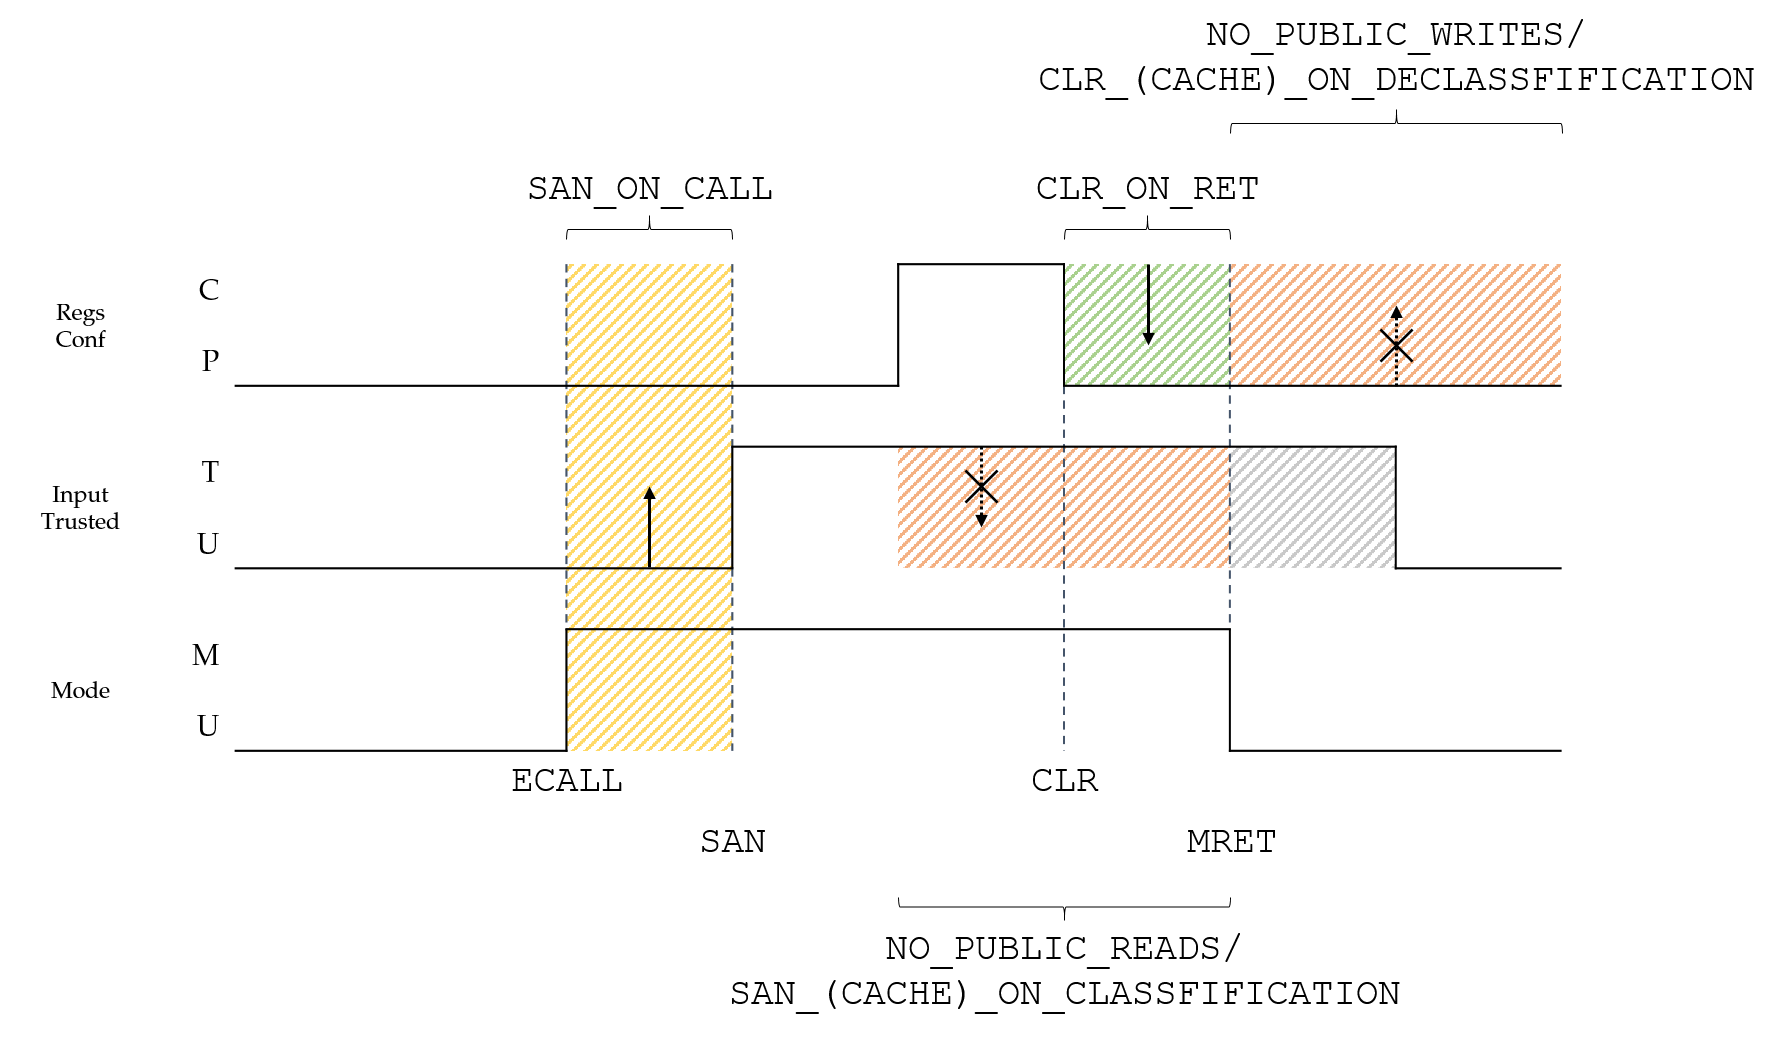
\includegraphics[width=\textwidth]{figures/assumptions.png}
    \caption{Assumptions visualized}
\end{figure}

%!TEX root = ../thesis.tex

\chapter{Discussion}
\label{chp:discussion}

In section \ref{sec:ifc-properties}, a set of \gls{ifc} properties based on the work in \cite{Ferraiuolo17} has been introduced; the set of these properties will be referred to as $ P $.
These properties were model checked, the main result of which was a set of rules $ R $ as presented in the previous chapter \ref{chp:results} .
What is the consequence of this?
The formal achievement of this thesis can be summarized as follows:
\begin{quote}
    It can be guaranteed that programs running on the MINRV8 architecture, e.g. \glspl{os}, are \textit{secure} (in the sense of not violating the \gls{ifc} properties $ P $) if they obey to the rules $ R $.
\end{quote}
But what does \enquote{secure} mean here besides not violating $ P $?
What is the \textit{actual} sense of security that can be guaranteed?

At this point, the class of vulnerabilities covered by these properties cannot be defined strictly.
However, the canaries these properties have been tested against in section \ref{sec:canaries}, exemplify this class of vulnerabilities.
Assessing the results of the approach to formally verify higher level properties of the MINRV8 architecture shall be subject of this section.
We will cover four aspects of our work:
\begin{itemize}
    \item Scope, i.e. what are the limits of our results,
    \item Trustworthiness, i.e. whether our results are sound,
    \item whether the model could have been implemented more abstractly,
    \item if there are alternatives to tracking information on a per-bit basis, and finally
    \item whether the results meet the self-imposed requirements as set up in chapter \ref{chp:introduction} and section \ref{sec:sum-background}.
\end{itemize}

Whereas the topics of the scope and trustworthiness of our work touch more general aspects of our work, the two questions following up on this reflect on the methodology of this thesis and will elaborate other possible approaches to our subject.

\section{Scope}
\label{sec:scope}

\subsection{Architecture}
\label{sec:discuss-arch}

MINRV8 is meant to be a reasonable abstraction of a real-world RISC-V architecture from a security standpoint.
However, up to this point nothing has been said about the limits of this abstraction.
With every abstraction, there is a small chance that it perfectly matches the concept that has been abstracted in regard to the purpose of the abstraction but in most cases, some corners are cut.
In this section, we will reflect on the limits of the MINRV8 architecture and its implementation.

In summary, the MINRV8 architecture knows three groups of instructions (cf. table \ref{tbl:min-arch-instrs}):
\begin{itemize}
    \item Computational instructions such as \minrv{Mov}, \minrv{And}, \minrv{Add}, etc.
    \item Memory instructions \minrv{Load} and \minrv{Store}
    \item System instructions \minrv{Ecall}, \minrv{Mret}, \minrv{Csrrs}, \minrv{Csrrc}
\end{itemize}

A reader, experienced in the field of microcontrollers or computer-architecture in general might wonder why our model does not include:
\begin{enumerate}
    \item Executable memory and a \gls{pc}
    \item Jump or branch instructions
\end{enumerate}

The reason for both of these points lies in the implementation of the model.
In the introduction of the MINRV8 architecture in section \ref{sec:minrv8} we mentioned that the idea of the architecture was tightly coupled to its implementation in nuXmv.
The design of the model had to answer the question: How can a stream of instructions be implemented?
nuXmv allows to think of the following options:
\begin{enumerate}
    \item \label{itm:exmem-frozen}
    Use \smv{FROZENVAR}s to model executable memory - a \smv{FROZENVAR} (frozen variable) is something like a constant in other programming languages but without a fixed value.
    nuXmv chooses the value on the first simulation step but does not change it afterwards.
    This is more efficient than using a plain \smv{VAR} and constraining it to not change, e.g. \smv{TRANS next(x) = x;}.
    \item \label{itm:exmem-var}
    Use \smv{VAR}s to model executable memory.
    In practice, this would mean that for memory to hold all instructions executed it would need to be much larger than the current 4 bytes.
    \item \label{itm:exmem-ivar}
    Finally, use \smv{IVAR}s to model the stream of instruction.
    This is the option we decided to go for as described in section \ref{sec:model-implementation}.
    Using input variables means that there is no model of executable memory.
    Instead, the input variables provided to the implementation model a stream of a fully decoded instruction on each transition of the simulated model.
    As such, the architecture does not need to worry \textit{where} these instructions come from.
\end{enumerate}

The decision towards using input variables as a model of the stream of instructions was made because of two reasons:
\begin{enumerate*}[label=\alph*)]
    \item in the prototyping phase of the model, it was quickly found out that using input variables led to significant boosts in performance, and
    \item using input variable simplified the implementation significantly.
\end{enumerate*}
Having used purely either frozen variables or variables would have increased the size of the state space to be traversed by nuXmv and would have introduced the necessity to implement instruction decoding increasing the complexity of the transition relation.
Furthermore, it would not have allowed for unbounded model checking of the architecture since the size of programs to be taken into consideration would have been bounded by the size of executable memory.

Yet, using input variables also has some downsides.
First and foremost, using input variables means that it is pointless to model a \gls{pc} or anything address related like return addresses, a dedicated \gls{lr} or \glspl{csr} such as \gls{mtvec}, the \gls{csr} holding the trap-vector base address, as without a model of executable memory there is nothing addresses could point to.
Instead, instructions will simply magically appear on each cycle of the processor model.
This means that the simulation is inaccurate in this regard which in itself is not a problem.
The model is supposed to be an abstraction.

\begin{figure}
    \centering
    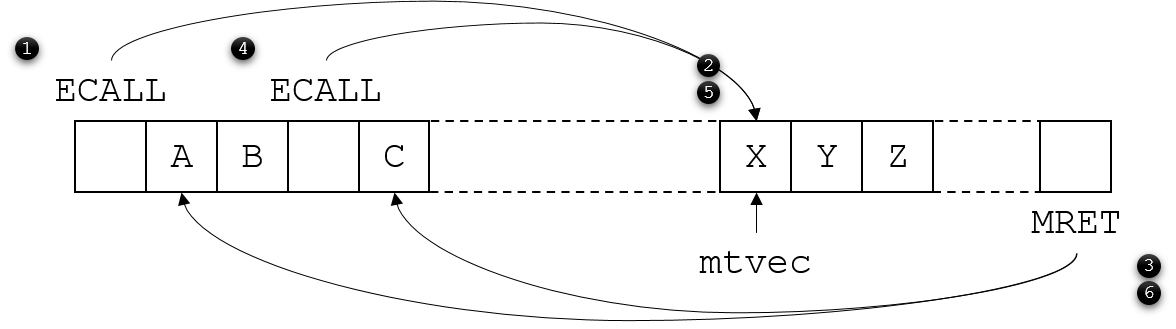
\includegraphics[width=0.7\textwidth]{figures/interrupt-flow.png}
    \caption{Program flow involving interrupts}
    \label{fig:interrupt-flow}
\end{figure}

Since it was decided to use input variables over a model of the \gls{mtvec} register and a \gls{pc}, the question now arises: How accurately is the implementation of the MINRV8 architecture capable of simulating real architectures?

In a nutshell, the use of input variables over (frozen) variables introduces a sense of non-determinism to the model of the MINRV8 architecture when it comes to handling interrupts and exceptions which is illustrated by the following example:
Consider some memory layout for the RISC-V architecture as depicted in figure \ref{fig:interrupt-flow} where code is executed from left to right starting with an \minrv{Ecall} instruction.
Executing this instruction triggers a shift in control to machine-mode which jumps to address \minrv{X} pointed to by the \gls{mtvec} register.
Then, the instructions at addresses \minrv{X} to \minrv{Z} and subsequent ones are executed until finally, a \minrv{Mret} instruction is read an executed which triggers a jump to address \minrv{A}.
Two instructions later, another \minrv{Ecall} instruction is executed, etc.
We would expect the order of instructions to be executed to look something like:

\begin{enumerate}
    \item First environment call: \lstinline[language=minrv8,mathescape=true]{Ecall, Load, Add, Store, $\dots$, Mret}
    \item Return: \lstinline[language=minrv8,mathescape=true]{Load, Mov}
    \item Second environment call: \lstinline[language=minrv8,mathescape=true]{Ecall, Load, Add, Store, $\dots$, Mret}
    \item Second return: \lstinline[language=minrv8,mathescape=true]{Slt, $\dots$}
\end{enumerate}
Where \minrv{Load, Add, Store} are the instructions located at addresses \minrv{X} to \minrv{Z} and \minrv{Load, Mov, Slt} the instructions located at addresses \minrv{A}, \minrv{B} and \minrv{C} respectively.

However, as input variables can not be constrained in nuXmv, there is no way to model that the instructions being executed on a trap always are equal, i.e. a valid stream of instructions as a sequence of input variable valuations to the model might be:
\begin{enumerate}
    \item First environment call: \lstinline[language=minrv8,mathescape=true]{Ecall, Load, Add, Store, $\dots$, Mret}
    \item Return: \lstinline[language=minrv8,mathescape=true]{Load, Mov}
    \item Second environment call: \lstinline[language=minrv8,mathescape=true]{Ecall, And, Sra, $\dots$, Mret}
    \item Second return: \lstinline[language=minrv8,mathescape=true]{Slt, $\dots$}
\end{enumerate}

Such a stream of instructions is not realistic without some program modifying the code located at \gls{mtvec} and as such \enquote{shouldn't} be considered when checking the \gls{ifc} properties.
One would expect to find the same code after an \minrv{Ecall} instruction being executed since in both cases, an architecture would jump to the respective interrupt handler\footnote{%
    To be precise, one would also need to take vectored interrupts into account (c.f. sec. \ref{sec:rv-priv-arch}) but even then, the issue applies.
}.
However, there also exists a sequence of input variable valuations that exactly matches a \enquote{real} stream of instructions where the instructions executed after an environment call coincide.

This illustrates one example for why the implementation of the MINRV8 \textit{abstracts} from real architectures.
In regard to program flow on traps, it can be expected that the model accurately comprises all expected streams of instructions but also includes many more one would naturally consider to be unrealistic.

The second concept, the abstract implementation of the MINRV8 architecture is missing are jump an branch instructions.
They are missing for the exact same reasons as described in the previous paragraphs.
Since the implementation does not support executable memory and as such does not support addresses, jumps and branches are pointless instructions.
This, however, does not turn out to be a fundamental problem.

The implementation might not be able to model programs including jumps and branches but the set of programs considered by nuXmv does include traces that include the same instructions that would have been executed when running a program with jumps and branches but without the jumps and branches.
We call such a trace a linearization\footnote{%
    Linearization is similar to function inlining supported by many compilers.
} of a program with jumps and branches.
Consider figure \ref{fig:jump-inlining} where in the upper half depicts an ordinary program, being executed from left to right and including jump instructions.
The respective counterpart to the program in the upper half is depicted in the lower half of figure \ref{fig:jump-inlining}.
This linearized counterpart is considered by nuXmv and the sequence of states generated by the linearized programs is equal to the sequence of states of the non-linearized program modulo \gls{pc} values - which is not modelled in nuXmv anyways.

\begin{figure}
    \centering
    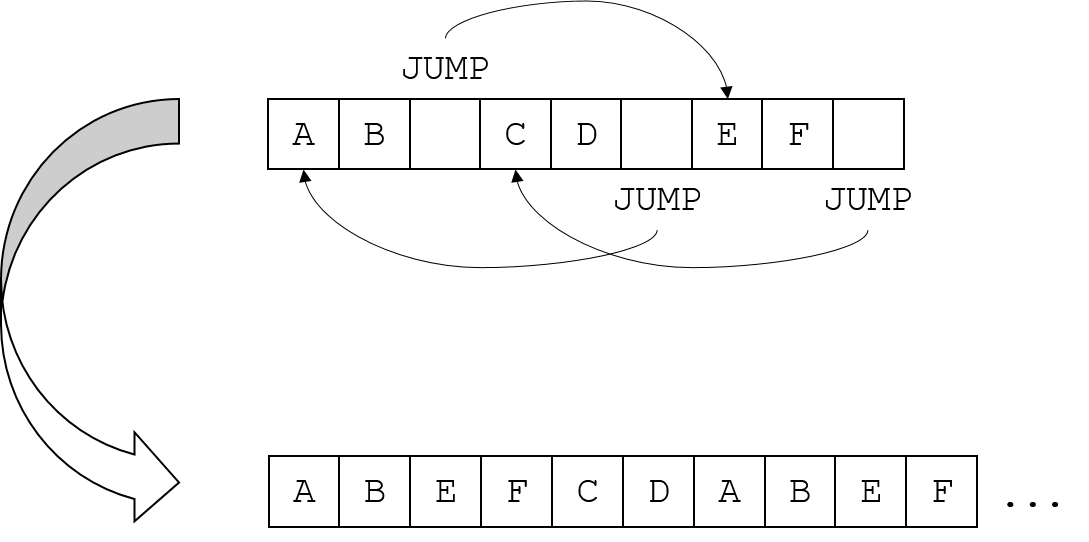
\includegraphics[width=0.7\textwidth]{figures/jump-free-programs.png}
    \caption{Jump linearization}
    \label{fig:jump-inlining}
\end{figure}

\paragraph{Summary}

Starting with the premise of this thesis, it was always clear that the MINRV8 architecture is a simplification.
This, though, is not a problem since by focusing on the very core, security related instructions allowed to implement a tractable and small model in nuXmv.
If one would add jump and branch instructions to the MINRV8 architecture, it'd be fully comparable to actual RISC-V architectures.
From this point of view, it is not a problem to apply the results of the verification process, i.e. the set of assumptions, to the RISC-V architecture.

The implementation of the MINRV8 architecture abstracted from real-world architectures in two main points:
\begin{enumerate}
    \item nuXmv does not guarantee stable behavior on \minrv{Ecall} instructions; this introduces a sense of non-determinism for which there are more programs considered by nuXmv than could actually be run on the MINRV8 architecture.
    This is not problematic because overabstracting the space of all programs $ P $ still leaves nuXmv considering all programs in $ P $.
    \item The implementation does not support jump or branch instructions.
    This is not problematic because programs including jumps can be linearized; such programs \textit{are} considered by nuXmv.
\end{enumerate}

This leaves us with good reasons to assume that programs considered by nuXmv, i.e. the set of programs quantified over when running proofs, is sufficiently close to the set of \enquote{real} programs of the MINRV8 architecture including jumps and branches.

\subsection{Assumptions}

Recall the requirements of the assumptions that have been laid out in section \ref{sec:sum-background}:
\begin{enumerate*}
    \item The assumptions must be non-trivial,
    \item the assumptions must only constrain machine-mode, and
    \item the assumptions must be practical and verifiable.
\end{enumerate*}

In this section, it will be investigated whether the assumptions that ultimately established the correctness of the information flow properties meet all these requirements.

Regarding point \ref{itm:assumptions-non-trivial}, it must be checked that neither are the assumptions contradictory nor do they trivially entail the information flow properties.
Recall that we were able to prove that \enquote{$ \text{assumptions} \Leftrightarrow \text{properties} $}.
In this case, the assumptions could only be contradictory if the properties are as well which they are obviously not as there are valid counter-examples to the properties when no assumptions are given.
On the other hand, recall that in section \ref{sec:canaries} we were able to make changes to the architecture such that \enquote{$ \neg(\text{assumptions} \Rightarrow \text{properties}) $} held.
This indicates that the assumption actually express something meaningful and do not trivially entail the information flow properties.

Point \ref{itm:assumptions-machine-mode} also is met by the assumptions introduced in section \ref{sec:assumptions}.
Whenever it is said that certain instructions must not be executed under certain circumstances, these formulas are guarded by the antecedent \smv{priv ->}.
Additionally, all other assumptions only constrain state transitions being under control of machine-mode only, such as changes to \glspl{csr} or state before machine-mode hands back control to user-mode.

For point \ref{itm:assumptions-verifiable}, meeting point \ref{itm:assumptions-machine-mode} is one step in the right direction.
However, it must remain an open question here whether the assumptions introduced in section \ref{sec:assumptions} can be applied to real-world systems in a verification scenario.
The problems behind this are illustrated by the \smv{SP_BANK} assumption introduced parallel to the SYSRET vulnerability in section \ref{sec:sysret}.
There are two aspects of the first part of this assumption which are noteworthy.
The relevant part of the \smv{SP_BANK} assumption is given in snippet \ref{snpt:sp-bank-p1}.

\begin{figure}
    \begin{lstlisting}[
        language=smv,
        caption={First part of the assumption \lstinline{SP_BANK}},
        label={snpt:sp-bank-p1}
    ]
        G (!priv & X priv -> X ( (*\label{ln:sp-call-priv}*)
            (priv -> !(op in { PUSH, POP }))
            U ((op = MRET & MPP = 0b_0) | sp[sp_sel] < $REGION0_SIZE (*\label{ln:sp-call-mret}*)
                ? !pmpcfg0.write & !pmpcfg0.read
                : !pmpcfg1.write & !pmpcfg1.read)
        )) &
    \end{lstlisting}
\end{figure}

Whilst working on this assumption, it was found that the specific implementation of two \textit{ideas} was critical to the presence of the SYSRET vulnerability, both:
\begin{enumerate}
    \item \label{itm:no-sysret-priv}
    replacing the expression \smv{!priv & X priv} in line \ref{ln:sp-call-priv} by \smv{(op = ECALL) | (bool(MIE) & bool(MEIP))} which is the actual condition under which a trap is taken and
    \item \label{itm:no-sysret-mret}
    omitting the expression \smv{(op = MRET & MPP = 0b_0)} in line \ref{ln:sp-call-mret}
\end{enumerate}
led to nuXmv not reporting the SYSRET vulnerability.
Why is that?

The first part of the \smv{SP_BANK} assumption states: \enquote{Whenever there is a switch from user- to machine-mode, latter can only use the \minrv{Push} or \minrv{Pop} instructions after having returned to user-mode or having ensured that the stack-pointer is safe}.
If the antecedent of this assumption would have been replaced by: \enquote{Whenever a trap is taken, \dots}, i.e. by \smv{(op = ECALL) | (bool(MIE) & bool(MEIP))}, the consequent would also have applied to cases where a trap was taken from machine-mode to machine-mode\footnote{
    Furthermore, it is noteworthy that the antecedent in the original assumption resembles a more result-driven approach to phrasing properties, i.e. talk about \textit{what} is happening, whereas the alternative discussed here resembles a more architecture-driven approach, i.e. talk about \textit{when} things are happening.
    The discussion, which of these approaches should be preferred is a topic on its own.
    In this thesis, we used both approaches but tried to stick to the result-driven approach whenever possible to keep the assumptions concise.
    In certain situations, however, it was more practical to go for the architecture-driven approach.

    A similar issue was discussed by \citeauthor{Reid17} when he elaborates how the properties he verified the ARM architecture against were phrased (cf. \cite[p.88:4]{Reid17}).
}.
Such a trap is critical for the SYSRET vulnerability as it interrupts machine-mode from properly returning to user-mode while already having set the stack-pointer back to user-mode.
The consequent also applying to traps from machine- to machine-mode in context of the MINRV8 architecture leads to machine-mode ensuring that the proper stack-pointer is setup correctly on \textit{all} traps rendering the SYSRET vulnerability impossible.
For example, the \glspl{os} being affected by the SYSRET vulnerability clearly did not set the stack-pointer on \textit{all} execution paths of the trap handler for the general protection fault.

The condition \smv{(op = MRET & MPP = 0b_0)} on the right-hand side of the \smv{U}-expression in line \ref{ln:sp-call-mret} equals telling machine-mode: \enquote{You can forget about not using the \minrv{Push} and \minrv{Pop} instructions after you have \textit{attempted} to return control to user-mode}.
For the same reasons as stated above, this part is critical.
Leaving this expression out would equal machine-mode having state persistent over user-mode-calls and -returns to and from machine-mode, by which machine-mode memorizes whether it has set the stack-pointer to user-mode or to machine-mode.
With such a mechanism in place, machine-mode could not be fooled into using the user-mode stack-pointer on any trap handler since it would first check this state.

These two examples stress that the precise phrasing of the assumptions is critical for both how realistic the assumptions are and how well they might be suited to serve as target for verification of actual code-bases.
While it would be sufficient to find a stronger precondition for these assumptions in existing code-bases, it is non-trivial whether such preconditions are easy to find or whether the assumptions might be rephrased such that they still grant the absence of information flow related bugs but are easier to verify in programs.
This topic, though, can't be handled as part of this thesis and as such marks future work.

\section{Trustworthiness}
\label{sec:trustworthiness}

Verification processes must not be arbitrary.
The core of verification is to enhance the trust in a given system.
For trust to arise, it is mandatory for the process itself to be trustworthy.

But what does \textit{trustworthy} mean?
\citeauthor{Piano} expressed discussed sense of trustworthiness in his blog post \citetitle{Piano} as:
\textcquote{Piano}{\textins{I}t is extremely difficult to argue convincingly that a verification result is correct. By \enquote{correct} I mean not only \enquote{mathematically sound} but also \enquote{the result is faithful to the intent of the verification effort.}}
Here, we will skip the aspect of technical soundness of this thesis, i.e. the question of whether the work presented in this thesis is without errors.
In consequence, the degree of trustworthiness of this thesis is determined by whether the results of the verification process actually enhance the confidence in the correctness of the MINRV8 architecture, i.e. rather than asking whether what we did was correct, we ask: did we do the \textit{right} thing?

A possible issue with verification is to make circular arguments (an example for this will be given in chapter \ref{chp:related-work}).
Verification engineers do not start their work out of nowhere.
They usually have a feel for what they attempt to verify and have some vulnerabilities in mind they try to tackle.
If the actual work of modeling a prototype and implementing a verification procedure is influenced by this too strongly, one might object:
\enquote{You were able to find vulnerability \textit{X} only because you knew that it was there. Your procedure is nothing but an abstracted simulation of known issues.}

This leads to another concern:
As with most programming, the verification process will tackle what is aimed for in some more general sense, i.e. when aiming to verify systems against certain bugs these are usually generalized to classes of related vulnerabilities.
But with such an approach, one can never be sure that there is no other class of vulnerabilities that was missed.
In other words: Does the verification procedure have blind spots?

It will now be investigated whether this work is touched by aforementioned two issues.

First, it will be investigated whether a circular argument has been made in this thesis.
Recall the steps that have been taken to verify the MINRV8 architecture against the information flow properties:
\begin{enumerate}
    \item \label{itm:step-minrv}
    Specify the MINRV8 architecture based on RISC-V
    \item \label{itm:step-semantics}
    Define information flow semantics for the instructions available on MINRV8
    \item \label{itm:step-properties}
    Use fields not being propagated in the information flow semantics and some intuition to state information flow properties
    \item \label{itm:step-loop}
    Enter a prove-refine loop until a fixpoint has been reached
    \item \label{itm:step-canaries}
    Test the model by subjecting it to vulnerabilities
\end{enumerate}

We find that steps \ref{itm:step-semantics} to \ref{itm:step-loop} are well founded by both theory and intuition and do obviously not face the risk of making a circular argument.
This, however, is less obvious for steps \ref{itm:step-minrv} and \ref{itm:step-canaries}.
In both cases, the selection of RISC-V features and instruction to include or vulnerabilities to test respectively can be doubted.

The work on this thesis was indeed influenced by the canaries the model was ultimately tested against, e.g. it was decided to implement a cache to be able to cover the cache poisoning attack, and vice versa: the selection of vulnerabilities to test the model against was based on the features implemented in it.
Despite the circular character of these two steps, we find that this is not an issue.
Steps \ref{itm:step-minrv} and \ref{itm:step-canaries} must be understood as a prototype of a verification procedure proposed in this thesis which is given by steps \ref{itm:step-semantics} to \ref{itm:step-loop}.
Having the setup to test these steps being derived via a methodology that is circular to some degree does not make the procedure itself circular.
The opposite is the case:
We find that the definition of information flow semantic, information flow properties and the prove-refine loop are all well founded and comprehensible, i.e. follow intuition.
On the other hand, we must admit that it is unknown whether there are blind spots to the verification procedure or more precisely: to the information flow properties.

We argue that our results are indeed trustworthy as we managed to show that our properties are not meaningless since they are able to detect both the SYSRET and the cache poisoning vulnerability and well founded in intuition.
But it is unclear
\begin{enumerate*}[label=\alph*)]
    \item which class of bugs or vulnerabilities can be detected by this procedure and
    \item whether this class covers \textit{all} vulnerabilities in the sense of \citeauthor{Piano}, i.e. \textcquote{Piano}{the result is faithful to the intent of the verification effort.}
\end{enumerate*}
We mark this problem as future work.

\section{Abstract Model}

One might ask, why it was decided to simulate all flows of information through the model of the MINRV8 architecture and indeed: In scope of this thesis, the actual content of registers is not mandatory, i.e. the actual contents of registers could be removed from the model such that only information flow tracking labels are tracked.
Register values do play a role when memory is indexed, but this could likely be abstracted by non-deterministically choosing a memory location to be targeted by loads and stores.

There are two reasons for why this decision was made.
Firstly, since the work of \citeauthor{Ferraiuolo17} \cite{Ferraiuolo17} was adopted where the authors did rely on precise values to track\footnote{%
    This is due to the fact that \gls{hdl} code is annotated.
    Or in other words: the authors did not have a chance to not track precise values.
} and performance of nuXmv did not mandate to shrink the model, it initially was decided to model values in the MINRV8 architecture.

However, secondly, working with concrete values has two benefits which might become important in future work.
\begin{enumerate}
    \item If the model ever was to be extended by jumps and branches, deterministic addresses are needed to model static code in executable memory.
    If not only loads and stores but also jumps and branches would use non-deterministic mechanisms to determine target addresses, modelling executable memory (cf. sec. \ref{sec:discuss-arch}) and for example interrupt handlers located in this very memory would be pointless to begin with.
    \item Concrete values lead to counter-examples being easier to interpret.
\end{enumerate}

With these two reasons at hand and the overall goal of this thesis to implement a prototype for a methodology to verify \glspl{isa}, we find that having modelled register values as opposed to abstractly tracking information flow labels only improves on the significance of our results.

\section{Per-Bit Information Flow Tracking}
\label{sec:per-bit-tracking}

Another issue is that in chapter \ref{chp:results} it was mentioned that counter-examples never involved flows of information where the bit-wise labels of values in the architecture was critical.
In other words: for this thesis, tracking only one bit for confidentiality and one bit for integrity for each register and memory address would suffice.
Initially, it was decided to track labels bit-wise because \begin{enumerate*}[label=\alph*)]
    \item we followed the approach of \citeauthor{Ferraiuolo17} \cite{Ferraiuolo17} which tracked information flow bit-wise as well,
    \item again, performance was sufficient to allow for it, and
    \item one couldn't have been sure prima facie non-bit-wise tracking of information would suffice.
\end{enumerate*}

Additionally, it can also be seen that computational instructions never played a major role in any counter-example.
These results suggest that in future work, if the model ever was to be expanded to a more accurate model of RISC-V and/or to a higher machine-word width and performance problems then are encountered, one could abstract the information flow tracking labels from bit- to word-wise labels.
This would decrease the size of the state space to be considered by nuXmv exponentially.
Additionally, one could remove instructions that only alter data but do not add \enquote{new} ways for information to flow.
E.g. the \minrv{Add} instruction - from a pure standpoint of \textit{where} information flows - adds nothing in comparison to the \minrv{Mov} instruction.
This option only shrinks the state space by a linear factor - nevertheless it might matter.

The gist of these findings is:
Whereas in the work of \citeauthor{Ferraiuolo17} \cite{Ferraiuolo17} tracking of each and every bit for a given system was crucial because the authors \textit{could not choose where bugs occur}, it seems that in our more-high level approach, for every bug \enquote{imaginable}, there is a very simple trace illustrating it: nuXmv is able to choose where a bug occurs since it quantifies over programs as opposed to the work of \citeauthor{Ferraiuolo17} where the program of interest is fixed.

\section{Requirements}
\label{sec:discuss-requirements}

In the introduction, three goals were set for this thesis: it was claimed that the approach presented as part of this thesis is \textit{viable}, i.e. feasible, realistic and generalizable, \textit{effective}, i.e. it is able to detect issues, and \textit{supplemental}, i.e. it enhances on related work.

All proofs were run on a laptop equipped with an Intel Core i7-7500U CPU and 8GB of RAM.
It is safe to say, that these are very moderate hardware requirements.
Proofs were conducted per property.
None of these proofs took more than 60s.
While we can give no clear count of working hours spent on this thesis, all of it was developed and written by a single person in no more than nine months.
During this time, this person did not solely work on this thesis.
In a non-research scenario one can assume that development would be more straight forward since it would not include the definition of an architecture.
Due to the exponential blow-up of binary encoded state spaces, there are no guarantees that this approach scales well to realistic and complete architectures.
However, there are two reasons which make seem likely that this approach does indeed scale.
Firstly, the proofs here were ran on a small machine and didn't take much time.
Secondly, in sections \ref{sec:per-bit-tracking} it was discussed that bit-wise tracking of information flow might be dropped, i.e. there is room for performance improvements.
All of this gives good reasons to believe that our approach is indeed \textit{viable} and could be applied to other architectures with reasonable effort.

To discuss the \textit{relevance} of this work, recall that in section \ref{sec:assumptions} it was shown that the implementation of the MINRV8 architecture models the property \enquote{assumptions $ \Leftrightarrow $ properties}.
This was put to a test by exposing the implementation to the cache poisoning or SYSRET vulnerability where it was found that it then does violate the properties as presented in section \ref{sec:ifc-properties}.
In other words: it was shown that the three properties \smv{MEMORY_OP_INTEGRITY}, \smv{CSR_INTEGRITY} and \smv{NO_LEAK} cover at least vulnerabilities related to the cache poisoning or SYSRET vulnerability without any manual intervention besides changing the architecture itself.
This marks the main result of this thesis and shows that our approach to verifying \glspl{isa} is \textit{effecitve}.
Furthermore, mitigations to these vulnerabilities can be verified using the same model.
It must be decided on a case by case basis whether a given violation of the information flow properties actually marks a vulnerability of the architecture leaving it with the need to be altered or marks a feature the risks of which must be controlled in software.

The discussion whether our work also is \textit{supplemental} will be postponed to a later stage.
In the following chapter \ref{chp:related-work}, related work will be presented.
Following up on this, this discussion will be picked up.

In addition to these self-imposed goals, it was also decided in section \ref{sec:verify-spec} to adopt the four design goals that were initially introduced in \cite{Reid17}.
These were defined to apply to high level properties for specifications and list as follows:
\begin{displaycquote}[pp.88:2-3]{Reid17}
    The central design challenge we face is to create a set of properties that:
    \begin{itemize}
        \item express the major guarantees that programmers depend on;
        \item are concise so that architects can easily review and remember the entire set of properties;
        \item are stable so that architectural extensions don't invalidate large numbers of rules;
        \item and that describe the architecture differently from existing specification to reduce the risk of common-mode failure.
    \end{itemize}
\end{displaycquote}

These objectives are met by our work:
\begin{itemize}
    \item The assumptions give rules for programmers of \glspl{os} and compilers that guarantee programs adhering to these do not violate basic information flow properties.
    \item Both assumptions and properties are small in number and short and can be expressed in intuitive natural language, hence are concise.
    \item The properties itself are completely architecture independent and as such stable.
    The assumptions are architecture dependent and rely on both instructions available and concrete semantics of these instructions.
    However, we feel subjectively that only basic mechanics are used and predict that the assumptions in a practical environment of an architecture should be relatively stable as well.
    \item The premise of information flow tracking on instruction level is to describe the architecture from a different point of view.
    It is therefore obvious that there is very little risk of common-mode failure.
\end{itemize}

%!TEX root = ../thesis.tex

\section{Related Work}
\label{sec:related-work}

As related work, we will consider seven papers - one of which will be investigated in detail.
Since this work founded itself both on \citetitle{Reid17} \cite{Reid17} and \citetitle{Ferraiuolo17} \cite{Ferraiuolo17} but both papers have been introduced in section \ref{sec:background} extensively, we won't consider them again in this section.
However, we will make an extensive comparison to the paper \citetitle{BradfieldS16} \cite{BradfieldS16} by \citeauthor{BradfieldS16} since this work is closest to ours.

The remaining six papers will be introduced as a group.
All related work covers verification\footnote{%
    It was a deliberate decision to not label all related work as \textit{formal} verification.
    E.g. \cite{Zhang15,SuhLZD04} do verify either properties or live program execution but do not use formal methods to accomplish this.
} of specifications or via information flow properties.
We found that related work can be characterized by four dimensions:
\begin{enumerate}
    \item It has either software or hardware as subject.
    \item It verifies either implementations or specifications.
    \item Verification is performed either live or statically.
    \item Information flow properties are either expressed directly or as non-interference properties.
\end{enumerate}

Given these categories, our work falls into the box of having hardware as subject, verifying a specification statically via direct information flow properties.

Two papers that do not consider hardware verification come from the Massachusetts Institute of Technology.
Firstly, \citeauthor{GordonKPGNR15} presented their tool DroidSafe for static analysis of information flow properties for android applications in their work \citetitle{GordonKPGNR15} \cite{GordonKPGNR15}.
Secondly, \citeauthor{SuhLZD04} proposed an approach to live track information on \gls{os} level tacking traps on security policy violations in \citetitle{SuhLZD04} \cite{SuhLZD04}.
It is quite far-fetched to call \cite{SuhLZD04} a paper about \textit{verification}.
Nonetheless, the approach is interesting and methodologically close to ours.

The authors in \cite{GordonKPGNR15} considered information flow privacy sensitive sources of information, e.g. unique device ID, SMS messages and other private file, to riskful sinks of information, e.g. the network, NFC and the local file system.
Both, sources and sinks, are guarded by the android \gls{api}.
The authors tracked information flow from sensitive sources to sensitives sinks which both are given by specific calls to methods of the android \gls{api}.
DroidSafe managed to detect at least 90\% of malicious information flows in selected benchmarks whilst reporting at most 13 false positives.

The approach in \cite{SuhLZD04} aims to prevent the misuse of programming errors such as buffer overflows or format strings.
As opposed to verifying the absence of such vulnerabilities, the authors track data from sensitive sources through instructions using per-byte bit labels to observe when such vulnerabilities are being targeted by attacker payloads from such sources.
As opposed to \cite{GordonKPGNR15}, where information was tracked from the \enquote{user} to the \enquote{outside world}, the flow of information here is the other way round: from the \enquote{outside world} to the \enquote{user}.
This is due to the fact that \cite{GordonKPGNR15} considered the domain of confidentiality and \cite{SuhLZD04} considered the domain of integrity when tracking information.
Additionally, this in in line with our work where we information flow properties regarding confidentiality stated that confidential data may not flow to user-mode (the \enquote{outside world}) and malicious data from user-mode may not flow to sensitive places in machine-mode (the \enquote{user} in this analogy).
Similarly to our work, the authors here also gave information flow semantics for each instruction available.
The authors proposed a simple security policy involving two rules:
\begin{displaycquote}{SuhLZD04}
    \textit{No instruction can be generated from I/O inputs}, and \textit{No I/O inputs and spurious values based on propagated inputs can be used as pointers unless they are bound-checked and added to an authentic pointer}.
\end{displaycquote}

Whereas the first can not be compared to the properties of this work meaningfully as executable memory is not modelled, the second comes remarkably close to the properties integrity property \ref{itm:prop-mem-i} which (in words of the authors of \cite{SuhLZD04}) states that no \enquote{spurios} value can be used as pointer.
The exception of bound-checks is implicitly modelled by the \smv{SAN_ON_*} assumptions in section \ref{sec:results} which mandate from machine-mode to sanitize register of spurious values before using them.
Such a sanitization might be implemented by boundary-checking.
% TODO: Double check whether this actually is true
Recall that the security lattice continues to track data as malicious only if both sources of an operation are malicious.
For example, comparing a value to a constant bound, loaded from trusted memory would set it to be trustworthy.

The approach of \cite{SuhLZD04} achieved a 100\% success rate in a benchmark and the authors claim that their approach has negligible performance impact.

These two papers were those related to software.
The other five papers are all related to hardware.
\citeauthor{Zhang15} considered the detection of hardware trojans in \citetitle{Zhang15} \cite{Zhang15}, i.e. parts of an integrated circuit that behave maliciously, can be activated by very few inputs and otherwise do not affect the functionality of the circuit.
They analyzed \gls{hdl} implementations of such integrated circuits searching for (mostly) unused parts in the design.
The techniques employed in this work do not come close to what has been used in this thesis.
However, one can view the detection of (mostly) unused parts of a design and information flow tracking as two sides of the same coin: whereas here, we strived for finding out where information can flow, the authors in \cite{Zhang15} aim for finding out where information (mostly) does not flow.

\citeauthor{Fox02} formally verified the \gls{arm} architecture by redundancy in \citetitle{Fox02} \cite{Fox02}.
% TODO: \gls{hol}
He implemented a formal model of the \gls{arm} architecture in the theorem prover HOL, using general first order logic for verification.
In this implementation, \citeauthor{Fox02} modelled two views on the \gls{arm} architecture: the \gls{isa} itself and the micro-architecture implementing this \gls{isa}.
\citeauthor{Fox02} used theorems expressing that there always must be some correspondence between runs of the \gls{isa}-world and runs of the micro-architecture-world.
If for a given list of instructions or a giving list of steps in the micro-architecture, no corresponding run of the opposite world can be found, the architecture itself must be flawed.
This work was picked up by \citeauthor{KhakpourSD13} in \citetitle{KhakpourSD13} \cite{KhakpourSD13}.
The authors of this work extended the implementation of \citeauthor{Fox02} proving three isolation properties of user- and machine-mode:
User-mode processes must only depend on process-accessible-resources, processes must only modify those memory regions they can access by a given MMU configuration and user-mode-processes must only execute code by calling machine-mode through a trap.
The first of these is a non-interference property.
In general, non-interference properties state that a given system (in this case: user-mode-processes) must not be influenced by certain values (in this case: non-user-mode-process accessible resources).
They are generally stated in the following form: whenever two initial states of the system agree on a list of selected values, the respective final states must also agree on these values.
This is an indirect way of expressing information flow properties.
As opposed to formalize: \enquote{information from source $ X $ must not flow to sink $ T $}, directly, non-interference properties state that \enquote{information from any illegitimate source must not flow to any sink}, hence must not be able to interfere computation.

In contrast to the work of this thesis, \citeauthor{KhakpourSD13} achieve to distinguish between multiple user-mode processes and in this way tackle a more broad problem.
In our work, we only considered the scenario of user-mode attacking machine-mode and not user-mode attacking different user-mode processes.
% TODO: mention in future work
It would be an interesting line of research to add an MMU to the model and extend the information flow properties accordingly.

On the other hand, \citeauthor{KhakpourSD13} do not give any sense for what these properties actually achieve when it comes to security.
It is not clear what kind of bugs concretely might be tackled by their properties; whilst they are intuitive and certainly should be met by the \gls{arm} architecture, it is unclear whether they actually guarantee any desirable characteristics of the architecture.
To some extent, these properties fall out of nowhere.
Whilst this critique to some extent also applies to our work, we think that the methodology of deriving the information flow properties as presented in section \ref{sec:checking} gives some sense of completeness to our properties which is missing from the work of \citeauthor{KhakpourSD13}.

Lastly, we consider the work of \citeauthor{Nienhuis19} in \citetitle{Nienhuis19} \cite{Nienhuis19}.
% TODO: \gls{cheri}
This work comes from a completely other direction: as opposed to verifying information flow properties in some existing architecture, the authors present a new architecture, CHERI, that guard memory accesses by \textit{capabilities}.
These capabilities allow processes to perform given actions on a given range of memory, specified per virtual address.
The development of CHERI was accompanied by formal methods and proofs to enhance the trust in this system.
The CHERI architecture is an attempt to equip an architecture with strong mechanisms of controlling information flow such that the trust in it is very high from the beginning, supported by formal proofs that certain desirable properties hold for this architecture.

\begin{table}
    \centering
    \begin{tabular}{| r | c c | c c | c c | c c |}
        \hline
        & \multicolumn{2}{c |}{Subject} & \multicolumn{2}{c |}{Level} & \multicolumn{2}{c |}{Context} & \multicolumn{2}{c |}{Information Flow} \\
        & SW & HW & Impl. & Spec. & Live & Static & Direct & Non-I. \\
        \cite{GordonKPGNR15} & \checkmark & & \checkmark & & & \checkmark & \checkmark & \\
        \hline
        \cite{SuhLZD04} & \checkmark & & \checkmark & & \checkmark & & \checkmark & \\
        \hline
        \cite{Zhang15} & & \checkmark & \checkmark & & & \checkmark & (\checkmark) & \\
        \hline
        \cite{Fox02} & & \checkmark & & \checkmark & & \checkmark & \multicolumn{2}{c |}{N/A} \\
        \hline
        \cite{KhakpourSD13} & & \checkmark & \checkmark & & & \checkmark & & \checkmark \\
        \hline
        \cite{Nienhuis19} & & \checkmark & & \checkmark & & \checkmark &\multicolumn{2}{c |}{N/A} \\
        \hline
        \cite{BradfieldS16} & & \checkmark & & \checkmark & & \checkmark & \multicolumn{2}{c |}{N/A} \\
        \hline
    \end{tabular}
\end{table}

%!TEX root = ../thesis.tex

\chapter{Conclusion}
\label{chp:conclusion}

Find an overview of this thesis as a whole in figure \ref{fig:overview}.
As a first step, the MINRV8 architecture inspired by the RISC-V architecture was defined and implemented in nuXmv in section \ref{sec:minrv8}.
In chapter \ref{chp:ifc}, information flow semantics and three information flow properties forming an information flow control in spirit of the work of \citeauthor{Ferraiuolo17} \cite{Ferraiuolo17} were developed.
The information flow semantics were used to augmented the model of the MINRV8 by information flow tracking.
In chapter \ref{chp:results} eight assumptions that, when implemented software running in machine-mode such as \glspl{os}, guarantee the absence of vulnerabilities covered by aforementioned information flow properties were presented.
Our model, the properties and the assumptions were evaluated by showing that taken together, they manage to detect both the cache poisoning \cite{Wojtczuk09} and the SYSRET vulnerability \cite{Dunlap19}.
Finally in chapter \ref{chp:discussion}, the limitations and the scope of our work were discussed and it was reflected whether our methodology is trustworthy.

\begin{figure}
    \centering
    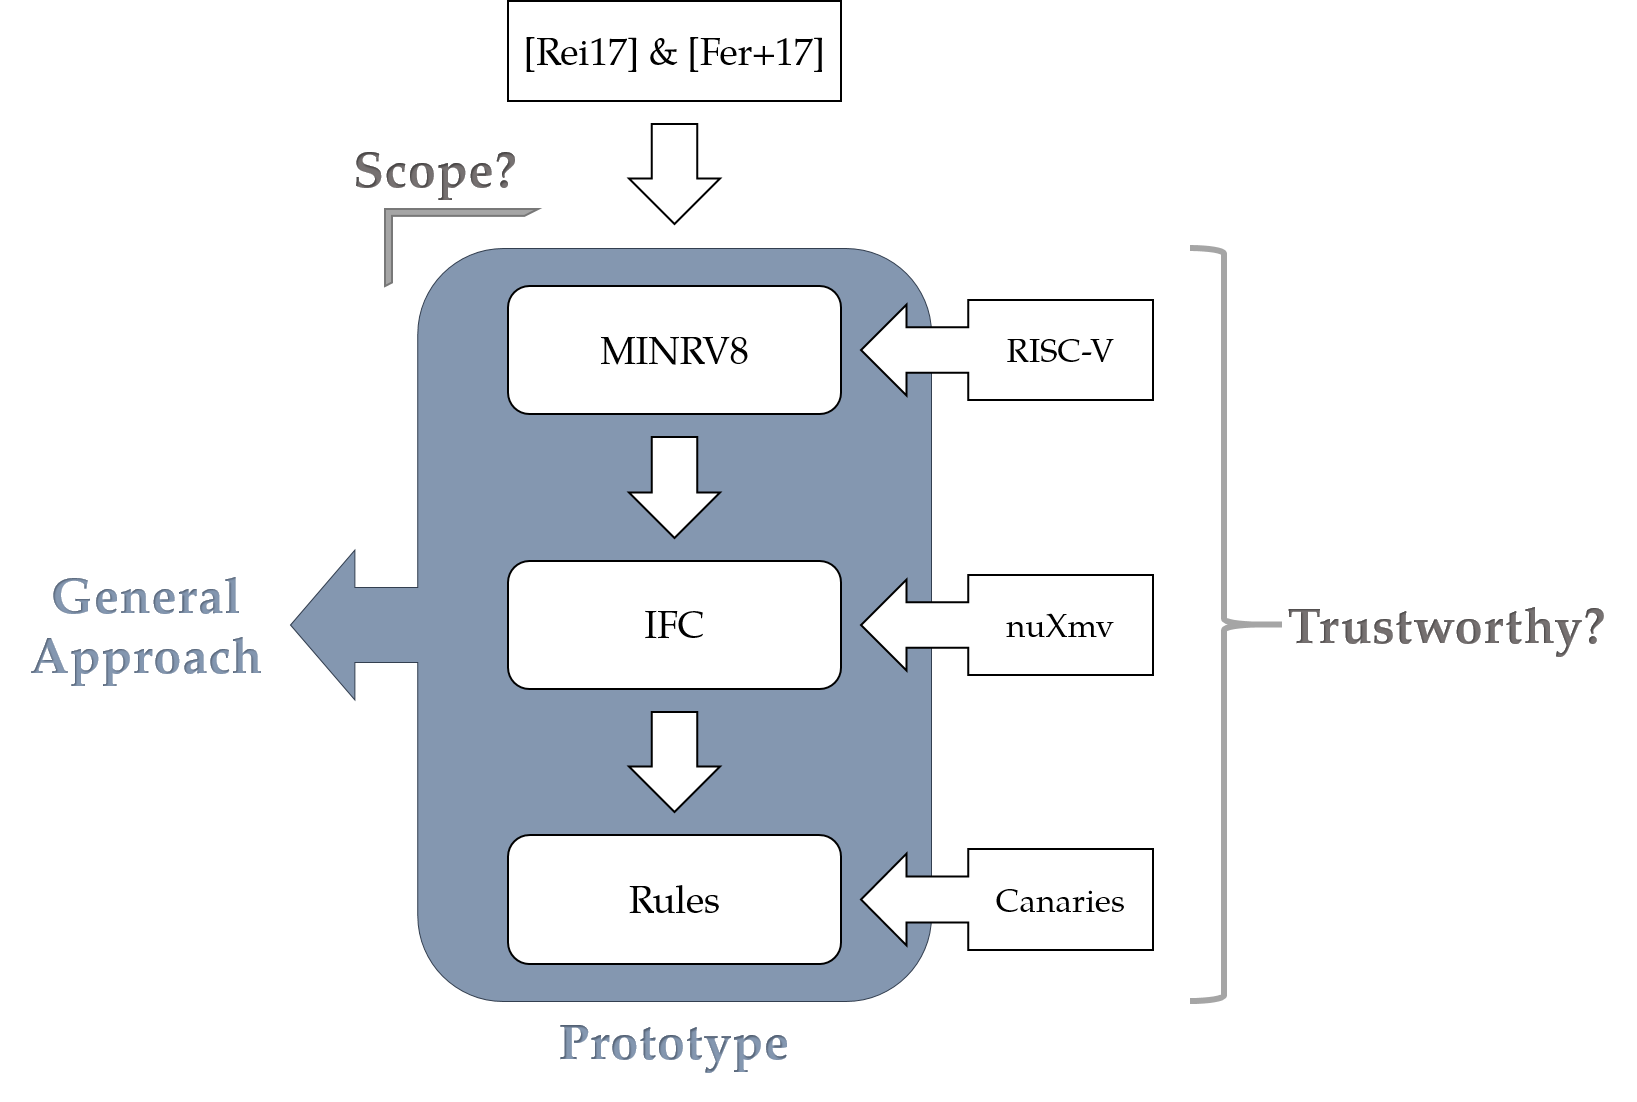
\includegraphics[width=\textwidth]{figures/thesis-overview.png}
    \caption{Thesis Overview}
    \label{fig:overview}
\end{figure}

Before a final summary of what has been achieved in this thesis will be given, we first recap all directions future work might take that were hinted towards throughout this thesis:
\begin{description}
    \item[Executable memory] First and foremost, the model could be enhanced by a model of executable memory to more closely resemble modern architectures.
    This was discussed extensively in section \ref{sec:discuss-arch}.
    \item[MMU] In light of \cite{KhakpourSD13} a model of an \gls{mmu} could be implemented to make use of information flow tracking on user-mode level.
    This was discussed in chapter \ref{chp:related-work}.
    \item[Machine-generated model] The model of the architecture that was implemented by hand in this thesis could be generated from existing machine-readable architectural specifications.
    For example, there are machine-readable versions of the ARM architecture; both \cite{Reid17,Fox02} either used or developed machine-readable specifications that might be used for this endeavor.
    For RISC-V, there also is a formal specification available \cite{RiscvSpecFormal}.
    Not implementing the model by hand would \begin{enumerate*}[label=\alph*)]
        \item possibly enhance the trust in the model itself, depending on the trust in the source and the translation procedure, and
        \item make the approach even more viable and stable towards architectural changes.
    \end{enumerate*}
    \item[Complete model] An obvious improvement of this work would be to enhance it by more instructions and use a bigger word-size.
    This would bring the model closer to real-world architectures but might also introduce performance issues.
    \item[Verification of assumptions] Finally, it could be investigated whether the assumptions introduced in context of the verification process serve as practical and sensible target of verification for compilers and/or \glspl{os}.
    It could be investigated whether code generated from compilers or \glspl{os} itself adheres to these assumptions.
    Applying the assumptions to the next level of abstraction in modern computing might lead to more easy and mainstream usage of formal verification in programming.
    Since these properties are stable for a given architecture, there could be off the shelf tools verifying programs for high-level correctness removing the need to tailor verification efforts per system to be verified.
\end{description}

Finally, the main contribution of this thesis is a new approach the verifying \glspl{isa} by higher-level information flow properties using a model checker.
This approach promises to take into account unbounded numbers of transitions, i.e. instructions, is non-redundant and architecture independent and results in either architectural changes to combat vulnerabilities or rules for e.g., \gls{os} or compiler engineers that are:
\begin{itemize}
    \item practical and verifiable themselves,
    \item concise, and
    \item stable.
\end{itemize}

This approach was applied to the MINRV8 to implement a prototype.
During this, three properties were found that lead to eight rules being stated.
These properties were broad enough to cover the cache poisoning and SYSRET vulnerabilities which both applied to the x86.


\printbibliography

\end{document}
